\documentclass[11pt,a4paper]{article}

\usepackage{iftex}
\ifPDFTeX
  \usepackage[utf8]{inputenc}
  \usepackage[T5]{fontenc}
  \usepackage{lmodern}
\else
  \usepackage{fontspec}
\fi
\usepackage[a4paper,margin=2.2cm]{geometry}
\usepackage{amsmath,amssymb}
\usepackage{enumitem}
\usepackage{xcolor}
\usepackage{tikz}
\usepackage{graphicx}
\graphicspath{{./}{../../}{../../results/}{../../demo/assets/canary/}}
\usepackage{float}
\usepackage[most]{tcolorbox}
\usepackage{eso-pic}
\usepackage{booktabs}
\usepackage{array}
\usepackage{longtable}
\usepackage{listings}
\usepackage{fancyhdr}
\usepackage{setspace}
\usepackage[colorlinks=true,linkcolor=blue!50!black,urlcolor=blue!50!black,unicode=true]{hyperref}
\usepackage{tocloft}
\sloppy
\setlength{\emergencystretch}{3em}
\hbadness=10000
\usepackage{needspace}

\setlength{\parindent}{0pt}
\setlength{\parskip}{4pt}
\setstretch{1.1}
\raggedbottom
\setlist{itemsep=2pt,topsep=3pt,parsep=1pt}
\setlist[itemize,1]{label=--,leftmargin=1.4em}
\setlist[itemize,2]{label={+)},leftmargin=1.6em}
\setlist[itemize,3]{label=\raisebox{0.2ex}{\scriptsize$\blacksquare$},leftmargin=1.4em}
\setlist[enumerate,1]{leftmargin=1.8em}

\renewcommand{\figurename}{Hình}
\renewcommand{\arraystretch}{1.15}

% ---------- Đầu trang, chân trang ----------
\setlength{\headheight}{14pt}
\pagestyle{fancy}
\fancyhf{}
\fancyhead[L]{\small\itshape Báo cáo phát hiện lỗi bo mạch in (PCB)}
\fancyfoot[C]{\small\thepage}
\renewcommand{\headrulewidth}{0.4pt}
\renewcommand{\footrulewidth}{0pt}

% ---------- Ký hiệu ----------
\newcommand{\pr}[1]{\mathit{#1}}
\newcommand{\xor}{\oplus}
% Trích dẫn tài liệu tham khảo: số thứ tự lấy tự động từ danh sách ở cuối báo cáo
\newcommand{\tlr}[1]{\ref{ref:#1}}

% ---------- Khung ----------
\tcbset{boxstyle/.style={enhanced,breakable,boxrule=0.6pt,arc=2pt,
  left=6pt,right=6pt,top=4pt,bottom=4pt,fonttitle=\bfseries\small}}
\newtcolorbox{dnghia}[1][]{boxstyle,colback=blue!4!white,colframe=blue!55!black,title={Định nghĩa},#1}
\newtcolorbox{dly}[1][]{boxstyle,colback=green!4!white,colframe=green!40!black,title={Định lý},#1}
\newtcolorbox{luuy}[1][]{boxstyle,colback=orange!6!white,colframe=orange!70!black,title={Lưu ý},#1}

% ---------- Mã nguồn (chú thích trong mã viết không dấu để biên dịch an toàn) ----------
\lstset{basicstyle=\ttfamily\small,frame=single,
  backgroundcolor=\color{gray!6},columns=fullflexible,keepspaces=true,
  showstringspaces=false,breaklines=true,aboveskip=4pt,belowskip=4pt,
  commentstyle=\color{green!35!black}}

% ---------- Bố cục ----------
\newcommand{\chuong}[1]{\clearpage\phantomsection\addcontentsline{toc}{section}{#1}{\centering\section*{#1}\par}}
\newcommand{\muc}[1]{\phantomsection\addcontentsline{toc}{subsection}{#1}\subsection*{#1}}
\newcommand{\chude}[1]{\subsubsection*{#1}}
\newcommand{\dang}[1]{\bigskip\noindent\textbf{\textcolor{blue!50!black}{#1}}\par\nopagebreak}
% Mục chưa thực hiện: giữ tiêu đề, để trống một khoảng. Điền nội dung sau khi làm xong.
\newcommand{\trong}[1][3cm]{\par\vspace{#1}}

% ---------- Mục lục ----------
\renewcommand{\contentsname}{MỤC LỤC}
\renewcommand{\cfttoctitlefont}{\centering\Huge\bfseries\color{blue!50!black}}
\renewcommand{\cftaftertoctitle}{\par\vspace{-4pt}%
  \noindent{\color{blue!50!black}\rule{\textwidth}{1.2pt}}}

% Cấp chương
\renewcommand{\cftsecfont}{\bfseries\color{blue!50!black}}
\renewcommand{\cftsecpagefont}{\bfseries\color{blue!50!black}}
\renewcommand{\cftsecleader}{\bfseries\cftdotfill{\cftdotsep}}
\setlength{\cftbeforesecskip}{9pt}
\setlength{\cftsecindent}{0em}
\setlength{\cftsecnumwidth}{0em}

% Cấp mục
\renewcommand{\cftsubsecfont}{\small}
\renewcommand{\cftsubsecpagefont}{\small}
\setlength{\cftbeforesubsecskip}{1pt}
\setlength{\cftsubsecindent}{1.8em}
\setlength{\cftsubsecnumwidth}{0em}

% ======================= Hình vẽ, thuật toán, đánh số theo chương =======================
% ---------- Hình vẽ, biểu đồ, thuật toán ----------
\usepackage{pgfplots}
\pgfplotsset{compat=1.16}
\usetikzlibrary{arrows.meta,positioning,shapes.geometric,fit,calc,backgrounds,decorations.pathreplacing,patterns}
\usepackage[font=small,labelfont=bf,labelsep=period,skip=6pt]{caption}
\usepackage{subcaption}
\usepackage[ruled,vlined,linesnumbered,noend]{algorithm2e}

% Đánh số hình, thuật toán, công thức theo chương (chuongso tăng trong \chuong)
\newcounter{chuongso}
\renewcommand{\thefigure}{\arabic{chuongso}.\arabic{figure}}
\renewcommand{\theHfigure}{\arabic{chuongso}.\arabic{figure}}
\renewcommand{\thealgocf}{\arabic{chuongso}.\arabic{algocf}}
\renewcommand{\theHalgocf}{\arabic{chuongso}.\arabic{algocf}}
\renewcommand{\thetable}{\arabic{chuongso}.\arabic{table}}
\renewcommand{\theHtable}{\arabic{chuongso}.\arabic{table}}
\renewcommand{\tablename}{Bảng}
\captionsetup[table]{position=top,skip=4pt}
\captionsetup[figure]{position=bottom}
\renewcommand{\theequation}{\arabic{chuongso}.\arabic{equation}}
\renewcommand{\theHequation}{\arabic{chuongso}.\arabic{equation}}

% Thuật toán bằng tiếng Việt
\SetAlgorithmName{Thuật toán}{thuật toán}{Danh mục thuật toán}
\SetAlgoCaptionSeparator{.}
\SetKwInput{KwIn}{Đầu vào}
\SetKwInput{KwOut}{Đầu ra}
\SetKw{KwRet}{trả về}
\SetKwIF{If}{ElseIf}{Else}{nếu}{thì}{nếu không, nếu}{nếu không}{}
\SetKwFor{ForEach}{với mỗi}{thực hiện}{}
\DontPrintSemicolon
\SetAlFnt{\small}
\SetAlCapFnt{\small}
\SetAlCapNameFnt{\small}
\SetCommentSty{textit}
\SetNlSty{}{}{}
\setlength{\algomargin}{1.2em}

% Hình, bảng ký hiệu dùng trong biểu đồ
\colorlet{chinh}{blue!50!black}
\definecolor{camdam}{RGB}{200,110,20}
\definecolor{luc}{RGB}{40,130,70}
\definecolor{nenmach}{RGB}{22,84,48}
\definecolor{dongmach}{RGB}{96,172,108}
\definecolor{chanmach}{RGB}{214,214,208}

\tikzset{
  khoi/.style={draw=chinh,fill=blue!6,rounded corners=2.5pt,thick,align=center,font=\scriptsize,
    minimum height=9mm,inner sep=3pt,text width=20mm},
  khoi vao/.style={khoi,draw=gray!70!black,fill=gray!12},
  khoi moi/.style={khoi,draw=camdam,fill=orange!14},
  khoi ra/.style={khoi,draw=luc,fill=green!10},
  khoi do/.style={khoi,draw=red!65!black,fill=red!7},
  quyet/.style={diamond,aspect=2.3,draw=camdam,fill=orange!10,thick,align=center,font=\scriptsize,
    inner sep=0pt,text width=26mm},
  mui/.style={-{Stealth[length=2.2mm,width=1.8mm]},thick,chinh},
  mui net/.style={-{Stealth[length=2.2mm,width=1.8mm]},thick,chinh,dashed},
  nhan/.style={font=\tiny\itshape,inner sep=1.5pt,text=black!70},
  tieude/.style={font=\footnotesize\bfseries,text=chinh,anchor=west},
}

% Biểu đồ cột dùng chung
\pgfplotsset{
  bieudo/.style={width=\linewidth,height=5.4cm,ybar,bar width=9pt,ymin=0,
    tick label style={font=\scriptsize},label style={font=\footnotesize},
    legend style={font=\scriptsize,draw=none,fill=none,at={(0.5,1.03)},anchor=south,legend columns=-1},
    ymajorgrids,grid style={gray!25},axis line style={gray!60},enlarge x limits=0.2,
    nodes near coords,every node near coord/.append style={font=\tiny,rotate=90,anchor=west},
    /pgf/number format/fixed,/pgf/number format/precision=4,/pgf/number format/fixed zerofill=false},
}

% Sơ đồ bo mạch minh hoạ (vẽ bằng TikZ, không phải ảnh thật của bộ dữ liệu)
% Quy ước: bo rộng 3.2, cao 2.2; #1=1 thêm lỗi (đứt mạch ở giữa, gai ở trên).
\newcommand{\vetmach}{(0.3,0.5)--(1.6,0.5)--(1.6,1.2)--(2.9,1.2) (0.3,1.8)--(2.9,1.8) (0.3,1.2)--(1.0,1.2) (2.2,0.5)--(2.9,0.5)}
\newcommand{\pcbmau}[1]{%
  \fill[nenmach,rounded corners=2pt] (0,0) rectangle (3.2,2.2);
  \draw[dongmach,line width=2.2pt,line cap=round,line join=round] \vetmach;
  \ifnum#1=1
    \fill[nenmach] (1.45,0.74) rectangle (1.75,0.96);
    \draw[dongmach,line width=0.9pt,line cap=round] (1.6,1.8)--(1.6,1.48);
  \fi
  \foreach \x/\y in {0.3/0.5,2.9/1.2,0.3/1.8,2.9/1.8,0.3/1.2,2.9/0.5}{%
    \fill[chanmach] (\x,\y) circle (0.14); \fill[nenmach] (\x,\y) circle (0.05);}%
}
\newcommand{\pcbnhi}[1]{%
  \fill[white] (0,0) rectangle (3.2,2.2); \draw[black!60] (0,0) rectangle (3.2,2.2);
  \draw[black,line width=2.2pt,line cap=round,line join=round] \vetmach;
  \ifnum#1=1
    \fill[white] (1.45,0.74) rectangle (1.75,0.96);
    \draw[black,line width=0.9pt,line cap=round] (1.6,1.8)--(1.6,1.48);
  \fi
  \foreach \x/\y in {0.3/0.5,2.9/1.2,0.3/1.8,2.9/1.8,0.3/1.2,2.9/0.5}{%
    \fill[black] (\x,\y) circle (0.14); \fill[white] (\x,\y) circle (0.05);}%
}
% #1=1: XOR thô (còn nhiễu); #1=0: sau median, đóng, mở (chỉ còn vùng lỗi)
\newcommand{\pcbxor}[1]{%
  \fill[black] (0,0) rectangle (3.2,2.2);
  \ifnum#1=1
    \fill[white] (1.5,0.76) rectangle (1.7,0.94);
    \fill[white] (1.57,1.48) rectangle (1.63,1.8);
    \foreach \x/\y in {0.62/0.55,1.05/0.45,1.9/0.5,2.5/1.25,2.1/1.75,0.8/1.82,0.5/1.15,2.6/0.45,1.65/1.0,2.95/1.75,0.35/0.9,1.3/1.3}{%
      \fill[white] (\x,\y) circle (0.022);}%
  \else
    \fill[white] (1.48,0.72) rectangle (1.72,0.98);
    \fill[white] (1.52,1.44) rectangle (1.68,1.82);
  \fi
}
% Hai vùng lỗi trên sơ đồ bo (khung ôm sát): đứt mạch và gai
\newcommand{\khungloi}[1]{%
  \draw[#1] (1.3,0.62) rectangle (1.9,1.08);
  \draw[#1] (1.38,1.34) rectangle (1.82,1.9);}

% Tham chiếu hình, thuật toán
\newcommand{\hinhref}[1]{Hình~\ref{fig:#1}}
\newcommand{\thuattoanref}[1]{Thuật toán~\ref{alg:#1}}
\newcommand{\bangref}[1]{Bảng~\ref{tab:#1}}

% Danh mục hình vẽ
\renewcommand{\listfigurename}{DANH MỤC HÌNH VẼ}
\renewcommand{\cftloftitlefont}{\centering\Huge\bfseries\color{blue!50!black}}
\renewcommand{\cftafterloftitle}{\par\vspace{-4pt}%
  \noindent{\color{blue!50!black}\rule{\textwidth}{1.2pt}}}
\renewcommand{\cftfigpresnum}{Hình }
\setlength{\cftfigindent}{0em}
\setlength{\cftfignumwidth}{4.8em}
\setlength{\cftbeforefigskip}{3pt}
\renewcommand{\cftfigfont}{\small}
\renewcommand{\cftfigpagefont}{\small}
% Danh mục bảng
\renewcommand{\listtablename}{DANH MỤC BẢNG}
\renewcommand{\cftlottitlefont}{\centering\Huge\bfseries\color{blue!50!black}}
\renewcommand{\cftafterlottitle}{\par\vspace{-4pt}%
  \noindent{\color{blue!50!black}\rule{\textwidth}{1.2pt}}}
\renewcommand{\cfttabpresnum}{Bảng }
\setlength{\cfttabindent}{0em}
\setlength{\cfttabnumwidth}{4.8em}
\setlength{\cftbeforetabskip}{3pt}
\renewcommand{\cfttabfont}{\small}
\renewcommand{\cfttabpagefont}{\small}
% Đặt số chương cho bộ đếm hình, thuật toán, công thức (gọi ngay sau mỗi CHƯƠNG n)
\newcommand{\sochuong}[1]{\setcounter{chuongso}{#1}\setcounter{figure}{0}\setcounter{table}{0}\setcounter{algocf}{0}\setcounter{equation}{0}}

\title{\textbf{BÁO CÁO PHÁT HIỆN LỖI BO MẠCH IN (PCB)}}
\author{}
\date{}

% ---------- Thông tin trên bìa: sửa tại đây ----------
\newcommand{\biamon}{Thị giác máy tính}
\newcommand{\biagv}{Hà Mạnh Toàn}
\newcommand{\biahoten}{Đồng Nguyên Khôi \hfill 24001677\par\vspace{3pt}Phan Thanh Lâm \hfill 24001680\par\vspace{3pt}Nguyễn Vân Mạnh \hfill 24001685}

\newcommand{\vienbia}{%
  \AddToShipoutPictureBG*{%
    \begin{tikzpicture}[remember picture,overlay]
      \draw[line width=2pt,blue!50!black]
        ([shift={(1.2cm,1.2cm)}]current page.south west) rectangle
        ([shift={(-1.2cm,-1.2cm)}]current page.north east);
      \draw[line width=0.6pt,blue!50!black]
        ([shift={(1.45cm,1.45cm)}]current page.south west) rectangle
        ([shift={(-1.45cm,-1.45cm)}]current page.north east);
    \end{tikzpicture}%
  }%
}

\begin{document}

\begin{titlepage}
\vienbia
\centering

{\large\bfseries ĐẠI HỌC QUỐC GIA HÀ NỘI\\[2pt]
TRƯỜNG ĐẠI HỌC KHOA HỌC TỰ NHIÊN\par}
\vspace{0.4cm}

\vspace*{0.3cm}
\IfFileExists{../../logo_hus.jpg}{\includegraphics[height=6cm]{../../logo_hus.jpg}\par}{\vspace{6cm}\par}
\vspace{0.5cm}

{\color{blue!50!black}\rule{0.8\textwidth}{1.2pt}}\\[0.6cm]
{\Huge\bfseries\color{blue!50!black} PHÁT HIỆN LỖI\\[6pt] BO MẠCH IN (PCB)\par}

{\large\itshape PCB Defect Detection with YOLOv8 and SIFT--XOR Image Differencing\par}
{\color{blue!50!black}\rule{0.8\textwidth}{1.2pt}}

\vspace{1.2cm}
{\LARGE\bfseries BÁO CÁO\par}
\vspace{0.8cm}

\begin{tabular}{@{}l@{\hspace{0.4cm}}p{9cm}@{}}
Học phần: & \biamon \\[6pt]
Giảng viên hướng dẫn: & \biagv \\[6pt]
Sinh viên thực hiện: & \biahoten \\[6pt]
Lớp: & \bialop \\
\end{tabular}

\vfill
{\normalsize Tháng 11 năm 2026\par}
\vspace{0.8cm}
\end{titlepage}

\pagenumbering{roman}

%=====================================================================
\chuong{LỜI CẢM ƠN}
%=====================================================================

Nhóm tác giả xin chân thành cảm ơn thầy Hà Mạnh Toàn, giảng viên hướng dẫn, đã định hướng đề tài và góp ý về cấu trúc báo cáo trong suốt quá trình thực hiện.

Chúng tôi cảm ơn nhóm tác giả bộ dữ liệu PCB của Đại học Bắc Kinh \tlr{huang} đã công bố dữ liệu và ảnh bo mẫu, là nền tảng cho toàn bộ thực nghiệm. Chúng tôi cũng cảm ơn cộng đồng mã nguồn mở đứng sau Ultralytics, PyTorch, OpenCV và Gradio, những công cụ giúp đề tài được cài đặt, kiểm thử và đóng gói trong thời gian ngắn.

Do thời gian và điều kiện thực hiện còn hạn chế, báo cáo khó tránh khỏi thiếu sót. Chúng tôi mong nhận được ý kiến đóng góp để hoàn thiện hơn.

\begin{flushright}
\textit{Hà Nội, tháng 11 năm 2026}\\[2pt]
\textbf{Nhóm tác giả}
\end{flushright}

%=====================================================================
\chuong{LỜI MỞ ĐẦU}
%=====================================================================

Bo mạch in (Printed Circuit Board, PCB) là nền tảng của hầu hết thiết bị điện tử. Một lỗi rất nhỏ trên đường mạch, như đứt mạch, chập mạch hay thiếu lỗ khoan, cũng đủ làm cả bo hoạt động sai hoặc hỏng. Vì vậy, kiểm tra ngoại quan bo mạch là một công đoạn không thể thiếu trong sản xuất. Công đoạn này nhiều nơi vẫn dựa vào mắt người: chậm, dễ mệt và phụ thuộc người kiểm tra, trong khi lỗi lại rất nhỏ so với kích thước bo.

Những năm gần đây, các mạng học sâu phát hiện đối tượng như YOLO cho kết quả cao trên bài toán này. Tuy nhiên, khi gặp bo mạch chưa từng thấy lúc huấn luyện, mô hình dễ nhầm chi tiết thiết kế cố định của bo với lỗi, làm số box thừa tăng mạnh. Ngược lại, kỹ thuật đối chiếu với ảnh bo mẫu không lỗi (căn chỉnh SIFT rồi XOR hai ảnh) nhìn thẳng vào chỗ khác biệt giữa hai ảnh, nhưng chỉ khoanh vùng thô.

Xuất phát từ nhận xét đó, đề tài kết hợp hai hướng: dùng YOLOv8 để phát hiện và phân loại lỗi, rồi dùng bản đồ khác biệt XOR giữa ảnh bo và ảnh bo mẫu để kiểm chứng từng box của YOLO. Dữ liệu được chia \textbf{theo bo mạch} để kết quả phản ánh khả năng với bo chưa từng thấy. Trên tập test gồm hai bo không nằm trong huấn luyện, bộ lọc XOR loại $348/368$ box thừa mà giữ nguyên $573$ box đúng, đưa precision từ $0.6089$ lên $0.9663$.

Báo cáo gồm mười chương, bố trí theo sườn của một đề tài nghiên cứu: mục tiêu, tổng quan tình hình nghiên cứu, sự cấp thiết, nội dung nghiên cứu chính, cách tiếp cận và kỹ thuật (Chương 1); các nội dung thực hiện và kết quả (Chương 2 đến Chương 8); tiến độ, sản phẩm và khả năng ứng dụng (Chương 9); kết luận và hướng phát triển (Chương 10).

\begin{luuy}[title={Quy ước khi đọc báo cáo}]
\begin{itemize}
  \item Số liệu lấy từ thư mục \texttt{configs/} và \texttt{results/} của mã nguồn, giữ nguyên chữ số thập phân.
  \item Tập \textbf{val} chỉ dùng để chọn mô hình, tham số và ngưỡng. Tập \textbf{test} chỉ chạy một lần cho phương án đã chốt.
  \item Mục 8.4 và 8.5 để trống vì cần hình ảnh hoặc liên kết thật chưa có ở thời điểm viết.
  \item Các sơ đồ mô tả quy trình và thuật toán (có ghi "sơ đồ minh hoạ" trong chú thích) vẽ bằng TikZ để giải thích ý tưởng, không phải ảnh thật của bộ dữ liệu. Các biểu đồ cột và điểm vẽ trực tiếp từ số liệu trong bảng của báo cáo.
  \item Cách đánh số mục (Mục 6, Mục 6.5) khớp với các chỗ trỏ đến báo cáo trong \texttt{README.md} và \texttt{demo/config.py}.
\end{itemize}
\end{luuy}

\begin{flushright}
\textit{Hà Nội, tháng 11 năm 2026}
\end{flushright}

%=====================================================================
\chuong{DANH MỤC TỪ VIẾT TẮT}
%=====================================================================

\begin{center}
\small
\begin{tabular}{l|p{12cm}}
\toprule
\textbf{Viết tắt} & \textbf{Ý nghĩa} \\ \midrule
PCB & Printed Circuit Board, bo mạch in \\
AOI & Automated Optical Inspection, kiểm tra quang học tự động \\
YOLO & You Only Look Once, họ mạng phát hiện đối tượng một giai đoạn \\
SIFT & Scale-Invariant Feature Transform, biến đổi đặc trưng bất biến theo tỉ lệ \\
SURF & Speeded-Up Robust Features, đặc trưng bền vững tăng tốc \\
FLANN & Fast Library for Approximate Nearest Neighbors, thư viện tìm láng giềng gần đúng \\
RANSAC & Random Sample Consensus, đồng thuận mẫu ngẫu nhiên \\
XOR & Phép hoặc loại trừ, lấy các pixel khác nhau giữa hai ảnh nhị phân \\
CNN & Convolutional Neural Network, mạng nơ-ron tích chập \\
IoU & Intersection over Union, tỉ lệ giao trên hợp của hai box \\
TP, FP, FN & Dự đoán đúng, báo thừa, bỏ sót \\
$P$, $R$, $F1$ & Precision (độ chính xác), recall (độ phủ), trung bình điều hòa của hai đại lượng đó \\
AP, mAP & Average Precision, mean Average Precision \\
mAP50, mAP50-95 & mAP ở IoU $0.5$; mAP trung bình trên IoU từ $0.5$ đến $0.95$, bước $0.05$ \\
CI & Continuous Integration, tích hợp liên tục \\
GPU & Graphics Processing Unit, bộ xử lý đồ họa \\ \bottomrule
\end{tabular}
\end{center}

\clearpage
\tableofcontents
\clearpage
\phantomsection\addcontentsline{toc}{section}{DANH MỤC HÌNH VẼ}
\listoffigures
\clearpage
\phantomsection\addcontentsline{toc}{section}{DANH MỤC BẢNG}
\listoftables
\bigskip\bigskip
\phantomsection\addcontentsline{toc}{section}{DANH MỤC THUẬT TOÁN}
{\centering{\Huge\bfseries\color{blue!50!black} DANH MỤC THUẬT TOÁN\par}\vspace{-4pt}%
 \noindent{\color{blue!50!black}\rule{\textwidth}{1.2pt}}\par}
\vspace{4pt}
\makeatletter\@starttoc{loa}\makeatother
\clearpage
\pagenumbering{arabic}

%=====================================================================
\chuong{CHƯƠNG 1: TỔNG QUAN ĐỀ TÀI}
\sochuong{1}
%=====================================================================

\muc{1.1. Mục tiêu đề tài}

\chude{1.1.1. Mục tiêu tổng quát}

Xây dựng và đánh giá một hệ thống phát hiện, định vị và phân loại sáu loại lỗi trên bo mạch in trần. Hệ thống kết hợp mạng học sâu YOLOv8 với phương pháp đối chiếu ảnh bo mẫu (căn chỉnh SIFT, nhị phân hóa, XOR), sao cho \textbf{ít báo thừa trên bo chưa từng thấy mà không làm mất lỗi thật}. Kết quả được đóng gói thành ứng dụng minh họa có thể chạy lại.

\chude{1.1.2. Mục tiêu cụ thể}

\begin{table}[H]
\centering
\small
\caption{Mục tiêu cụ thể và kết quả đạt được}\label{tab:muctieu}
\begin{tabular}{c|>{\raggedright\arraybackslash}p{6.2cm}|>{\raggedright\arraybackslash}p{6.0cm}}
\toprule
\textbf{TT} & \textbf{Mục tiêu cụ thể} & \textbf{Kết quả đạt được} \\ \midrule
1 & Chuẩn bị dữ liệu: đổi nhãn VOC sang YOLO, chia theo bo ($6/2/2$), kiểm toán rò rỉ (Chương 2) & Không có bo nào xuất hiện ở hơn một tập (180 dòng kiểm toán) \\ \midrule
2 & Huấn luyện và so sánh YOLOv8, chọn mô hình trên val (Chương 3, 5) & Chọn \texttt{pcb\_v8s\_board}; test mAP50 $0.9720$ \\ \midrule
3 & Cài đặt đường SIFT + XOR và bộ phân loại ảnh cắt (Chương 4, 5) & Box XOR: F1 $0.6376$ ở IoU $0.5$ (test); phân loại đúng $0.9169$ trên box tìm được \\ \midrule
4 & Phân tích lỗi bộ phát hiện, chọn ngưỡng theo lớp (Chương 6) & Precision test thấp do box thừa ở chi tiết cố định của bo \\ \midrule
5 & Đề xuất và đánh giá bộ lọc YOLO + XOR (Chương 7) & Box thừa $368 \to 20$, giữ nguyên $573$ box đúng; $P$ $0.6089 \to 0.9663$ \\ \midrule
6 & Xây dựng demo, kiểm thử, đóng gói (Chương 8) & Demo Gradio 4 chế độ, 32 hàm kiểm thử, CI, Docker \\ \bottomrule
\end{tabular}
\end{table}

\muc{1.2. Tổng quan tình hình nghiên cứu thuộc lĩnh vực đề tài}

\chude{1.2.1. Tình hình nghiên cứu ngoài nước}

\textbf{Hướng đối chiếu ảnh mẫu.} Khảo sát của Moganti và cộng sự \tlr{moganti} hệ thống hóa các thuật toán kiểm tra PCB bằng thị giác máy tính. Một nhóm lớn là các phương pháp đối chiếu với ảnh mẫu không lỗi: căn chỉnh ảnh kiểm tra, rồi trừ hoặc XOR với ảnh mẫu để lộ vùng khác biệt. Huang và Wei \tlr{huang} công bố bộ dữ liệu sáu loại lỗi (với $2953$ vùng lỗi có nhãn box) và đề xuất đường xử lý: căn chỉnh bằng SURF, nhị phân hóa thích ứng, XOR, lọc hình thái để định vị lỗi, sau đó phân loại ảnh cắt bằng một CNN lấy cảm hứng từ DenseNet. Bộ dữ liệu này về sau được nhiều nghiên cứu dùng làm chuẩn so sánh.

\textbf{Hướng phát hiện đối tượng bằng học sâu.} Faster R-CNN \tlr{ren} (hai giai đoạn) và YOLO \tlr{redmon} (một giai đoạn) là hai họ mạng được dùng nhiều nhất. Ding và cộng sự \tlr{ding} đề xuất TDD-Net, mạng phát hiện lỗi nhỏ trên PCB. Họ YOLOv8 \tlr{ultralytics} được áp dụng rộng rãi nhờ tốc độ và độ chính xác. Li và cộng sự \tlr{li} cải tiến YOLOv8 bằng cắt tỉa và mạng nhẹ, đạt mAP0.5 $99.32\%$ trên PKU-Market-PCB với $0.67$ triệu tham số.

\textbf{Hướng kết hợp ảnh tham chiếu với học sâu.} RefDiffNet \tlr{refdiff} (2026) là mô-đun tăng cường đặt trước bộ phát hiện: nó so sánh ảnh lỗi với ảnh tham chiếu đã căn chỉnh để làm nổi vùng lỗi, rồi đưa vào các bộ phát hiện như YOLOv8 hay Faster R-CNN; tác giả báo cáo cải thiện F1 và mAP trên DeepPCB và HRIPCB. Đề tài này đi theo cùng ý tưởng dùng ảnh tham chiếu, nhưng theo cách khác: ảnh mẫu được dùng \emph{sau} bộ phát hiện, để kiểm chứng từng box đầu ra.

\chude{1.2.2. Tình hình nghiên cứu trong nước}

Trong phạm vi các tạp chí khoa học trong nước tra cứu được, các công trình về kiểm tra bo mạch có thể chia thành hai nhóm.

\begin{itemize}
  \item \textbf{Đối chiếu bằng xử lý ảnh cổ điển.} Nguyễn Việt Thắng và cộng sự \tlr{thang} (2016) kiểm tra linh kiện thiếu trên bo lắp ráp: lưu ảnh bo mẫu, căn chỉnh bằng so khớp mẫu (template matching) rồi so histogram từng linh kiện.
  \item \textbf{Học sâu cho linh kiện trên bo lắp ráp.} Nguyễn Văn Trường và Nguyễn Đức Linh \tlr{truong} (2020) dùng Darknet-53 nhận dạng linh kiện, đạt khoảng $96\%$ trong điều kiện ánh sáng tốt, nền trắng, xử lý $120$ bo mỗi giờ. Nguyễn Ngọc Đức và cộng sự \tlr{duc} (2025) cải tiến YOLOv5 bằng mô-đun chú ý CBAM trên bộ dữ liệu tự xây dựng, đạt $97\%$ trong cùng kiểu điều kiện.
  \item \textbf{Lỗi trên bo trần.} Phạm Thu Hà và cộng sự \tlr{ha} (2025) so sánh Faster R-CNN và YOLOv8 trên chính bộ dữ liệu của Đại học Bắc Kinh ($693$ ảnh gốc, sáu loại lỗi), sau khi tăng cường dữ liệu và cắt thành ảnh $600\times600$. Faster R-CNN đạt khoảng $99.6\%$ độ chính xác ở $1.37$ s mỗi khung; YOLOv8 đạt $95\%$ ở $0.26$ s mỗi khung.
\end{itemize}

\textbf{Nhận xét.} Các công trình trong nước nêu trên chủ yếu dùng một bộ phát hiện học sâu đơn lẻ, hoặc đối chiếu cổ điển cho linh kiện. Trong phạm vi tra cứu, chưa thấy công trình dùng ảnh bo mẫu để kiểm chứng đầu ra của bộ phát hiện học sâu trên bo trần, và đánh giá với dữ liệu chia theo bo.

\needspace{20\baselineskip}
\begin{center}
\small
\begin{longtable}{>{\raggedright\arraybackslash}p{2.7cm}|>{\raggedright\arraybackslash}p{3.1cm}|>{\raggedright\arraybackslash}p{3.7cm}|>{\raggedright\arraybackslash}p{3.9cm}}
\caption{Tổng hợp các công trình liên quan}\label{tab:congtrinh}\\
\toprule
\textbf{Công trình} & \textbf{Đối tượng, dữ liệu} & \textbf{Phương pháp} & \textbf{Điểm chính} \\ \midrule
\endfirsthead
\toprule
\textbf{Công trình} & \textbf{Đối tượng, dữ liệu} & \textbf{Phương pháp} & \textbf{Điểm chính} \\ \midrule
\endhead
Huang, Wei (2019) \tlr{huang} & bo trần, 6 loại lỗi & căn chỉnh SURF, XOR, CNN phân loại & công bố dữ liệu; hướng đối chiếu ảnh mẫu \\ \midrule
Ding và cs. (2019) \tlr{ding} & bo trần & TDD-Net, phát hiện lỗi nhỏ & mạng chuyên cho lỗi nhỏ trên PCB \\ \midrule
Li và cs. (2025) \tlr{li} & PKU-Market-PCB, DeepPCB & YOLOv8 cắt tỉa, mạng nhẹ & mAP0.5 $99.32\%$; $0.67$ triệu tham số \\ \midrule
Edula và cs. (2026) \tlr{refdiff} & DeepPCB, HRIPCB & mô-đun so ảnh tham chiếu trước bộ phát hiện & tăng F1, mAP trên nhiều bộ phát hiện \\ \midrule
Nguyễn Việt Thắng và cs. (2016) \tlr{thang} & linh kiện trên bo lắp ráp & so khớp mẫu, so histogram & phát hiện thiếu linh kiện \\ \midrule
Nguyễn Văn Trường, Nguyễn Đức Linh (2020) \tlr{truong} & linh kiện, ảnh tự thu & Darknet-53 & khoảng $96\%$; $120$ bo/giờ \\ \midrule
Nguyễn Ngọc Đức và cs. (2025) \tlr{duc} & linh kiện, dữ liệu tự xây dựng & YOLOv5 + CBAM & $97\%$ (ánh sáng tốt, nền trắng) \\ \midrule
Phạm Thu Hà và cs. (2025) \tlr{ha} & dữ liệu Bắc Kinh, ảnh $600\times600$ & Faster R-CNN so với YOLOv8 & $99.6\%$ ($1.37$ s) so với $95\%$ ($0.26$ s) \\ \midrule
\textbf{Đề tài này} & bo trần, 6 loại lỗi, chia theo bo & YOLOv8s + SIFT--XOR + lọc XOR & test: $P$ $0.9663$, $R$ $0.9534$, $F1$ $0.9598$ \\ \bottomrule
\end{longtable}
\end{center}

\begin{luuy}
Số liệu trong bảng do từng công trình tự công bố, với dữ liệu và cách đo khác nhau (độ chính xác, mAP, $F1$), nên \textbf{không so trực tiếp} giữa các dòng. Số của đề tài này tính gộp, IoU $0.5$, khớp cùng lớp, trên hai bo test chưa từng thấy (Mục 7.3).
\end{luuy}

\muc{1.3. Sự cấp thiết của vấn đề nghiên cứu}

\begin{itemize}
  \item \textbf{Vai trò của kiểm tra bo mạch.} Lỗi trên đường mạch hoặc lỗ khoan làm cả thiết bị hỏng, nên phải được phát hiện trước khi lắp ráp. Sáu loại lỗi của đề tài (Mục 1.5.1) đều rất nhỏ so với kích thước bo, ảnh chụp có độ phân giải cao (hơn $2500$ px mỗi cạnh).
  \item \textbf{Kiểm tra bằng mắt người} chậm, dễ mệt và thiếu nhất quán, khó đáp ứng khi số lượng bo lớn.
  \item \textbf{Bộ phát hiện học sâu có điểm yếu rõ trên bo mới.} Kết quả của đề tài cho thấy precision của YOLOv8s giảm từ $0.9752$ (val) xuống $0.8543$ (test) khi gặp bo chưa từng thấy; box thừa lặp lại ở cùng một vị trí trên nhiều ảnh của một bo (Mục 6.4). Một hệ thống báo thừa nhiều sẽ buộc người kiểm tra duyệt lại, làm mất lợi ích của tự động hóa.
  \item \textbf{Ảnh bo mẫu thường có sẵn trong sản xuất}, nhưng chưa được tận dụng để kiểm chứng đầu ra của bộ phát hiện. Đề tài khai thác đúng khoảng trống này (Chương 7).
  \item \textbf{Thiếu công trình trong nước đánh giá chặt chẽ.} Trong phạm vi tra cứu (Mục 1.2.2), chưa thấy công trình chia dữ liệu theo bo hay dùng ảnh mẫu để lọc box. Đề tài cũng cung cấp mã nguồn, kết quả và demo có thể chạy lại, phục vụ nghiên cứu và giảng dạy.
\end{itemize}

\muc{1.4. Những nội dung nghiên cứu chính}

\begin{enumerate}
  \item \textbf{Dữ liệu và cách chia} (Chương 2): chuyển nhãn Pascal VOC sang YOLO; chia $10$ bo theo tỉ lệ $6/2/2$ để loại rò rỉ theo bo; kiểm toán rò rỉ; phát hiện và sửa lỗi hoán vị tên lớp.
  \item \textbf{Huấn luyện YOLOv8} (Chương 3): so sánh v8s và v8n, \texttt{imgsz} 1024 và 640; nguyên tắc dùng val để chọn và test để báo cáo.
  \item \textbf{Đường SIFT + XOR và bộ phân loại} (Chương 4): căn chỉnh, nhị phân hóa, XOR, khoanh vùng; ba cải tiến so với bản gốc; phân loại ảnh cắt bằng YOLOv8n-cls.
  \item \textbf{Kết quả và phân tích lỗi} (Chương 5, 6): so sánh các lần chạy, kết quả test, nguồn gốc của box thừa, ngưỡng độ tin cậy theo lớp.
  \item \textbf{Kết hợp YOLO + XOR} (Chương 7): quy tắc lọc box bằng bản đồ khác biệt, chọn tham số trên val, đánh giá trên test.
  \item \textbf{Demo và kiểm thử} (Chương 8): ứng dụng Gradio, cơ chế an toàn, kiểm thử, CI, đóng gói.
\end{enumerate}

\muc{1.5. Cách tiếp cận, phương pháp nghiên cứu và kỹ thuật sử dụng}

\chude{1.5.1. Bài toán}

\begin{itemize}
  \item \textbf{Đầu vào:} ảnh chụp một bo mạch in có lỗi.
  \item \textbf{Đầu ra:} vị trí (bounding box) và loại của từng lỗi trên ảnh.
  \item \textbf{Sáu loại lỗi:}
\end{itemize}
\begin{table}[H]
\centering
\small
\caption{Sáu loại lỗi của đề tài}\label{tab:saulop}
\begin{tabular}{c|l|p{9cm}}
\toprule
\textbf{Id} & \textbf{Lớp} & \textbf{Mô tả ngắn} \\ \midrule
0 & Missing Hole & lỗ khoan bị thiếu \\
1 & Mouse Bite & mép đường mạch bị khuyết, nham nhở \\
2 & Open Circuit & đường mạch bị đứt (hở mạch) \\
3 & Short & hai đường mạch bị nối nhầm (chập) \\
4 & Spur & gai đồng nhô ra từ đường mạch \\
5 & Spurious Copper & mảng đồng thừa, không thuộc thiết kế \\ \bottomrule
\end{tabular}
\end{table}
Id lớp đánh số theo thứ tự abc của tên lớp (xem Mục 2.2).

\hinhref{sauloi} minh hoạ sáu loại lỗi trên một đoạn mạch đơn giản.

\begin{figure}[H]
\centering
\begin{tikzpicture}[x=1cm,y=1cm,scale=0.92,transform shape]
\tikzset{pan/.style={},
  loi/.style={red!80!black,thick,dashed},
  duong/.style={dongmach,line width=3pt,line cap=butt},
  nhanloi/.style={font=\scriptsize,align=center,text width=3.6cm}}
% (a) Missing Hole
\begin{scope}[shift={(0,0)}]
 \fill[nenmach,rounded corners=2pt] (0,0) rectangle (3.2,2.2);
 \draw[duong] (0,1.1)--(1.0,1.1); \draw[duong] (2.2,1.1)--(3.2,1.1);
 \fill[dongmach] (1.6,1.1) circle (0.62);
 \draw[white,dotted,thick] (1.6,1.1) circle (0.16);
 \draw[loi] (0.85,0.35) rectangle (2.35,1.85);
 \node[nhanloi] at (1.6,-0.5) {(a) \textbf{Missing Hole}\\lỗ khoan bị thiếu};
\end{scope}
% (b) Mouse Bite
\begin{scope}[shift={(4.7,0)}]
 \fill[nenmach,rounded corners=2pt] (0,0) rectangle (3.2,2.2);
 \fill[dongmach] (0,0.85) rectangle (3.2,1.35);
 \foreach \x in {1.15,1.4,1.65,1.9}{\fill[nenmach] (\x,1.35) circle (0.09);}
 \foreach \x in {1.3,1.55,1.8}{\fill[nenmach] (\x,0.85) circle (0.09);}
 \draw[loi] (0.95,0.6) rectangle (2.25,1.6);
 \node[nhanloi] at (1.6,-0.5) {(b) \textbf{Mouse Bite}\\mép mạch bị khuyết};
\end{scope}
% (c) Open Circuit
\begin{scope}[shift={(9.4,0)}]
 \fill[nenmach,rounded corners=2pt] (0,0) rectangle (3.2,2.2);
 \fill[dongmach] (0,0.9) rectangle (1.35,1.3); \fill[dongmach] (1.85,0.9) rectangle (3.2,1.3);
 \draw[loi] (1.1,0.6) rectangle (2.1,1.6);
 \node[nhanloi] at (1.6,-0.5) {(c) \textbf{Open Circuit}\\đường mạch bị đứt};
\end{scope}
% (d) Short
\begin{scope}[shift={(0,-3.4)}]
 \fill[nenmach,rounded corners=2pt] (0,0) rectangle (3.2,2.2);
 \fill[dongmach] (0,0.35) rectangle (3.2,0.75); \fill[dongmach] (0,1.45) rectangle (3.2,1.85);
 \fill[dongmach] (1.35,0.75) rectangle (1.85,1.45);
 \draw[loi] (1.0,0.55) rectangle (2.2,1.65);
 \node[nhanloi] at (1.6,-0.5) {(d) \textbf{Short}\\hai đường mạch bị chập};
\end{scope}
% (e) Spur
\begin{scope}[shift={(4.7,-3.4)}]
 \fill[nenmach,rounded corners=2pt] (0,0) rectangle (3.2,2.2);
 \fill[dongmach] (0,0.55) rectangle (3.2,0.95);
 \fill[dongmach] (1.35,0.95)--(1.62,1.8)--(1.8,0.95)--cycle;
 \draw[loi] (1.1,0.8) rectangle (2.05,1.95);
 \node[nhanloi] at (1.6,-0.5) {(e) \textbf{Spur}\\gai đồng nhô ra};
\end{scope}
% (f) Spurious Copper
\begin{scope}[shift={(9.4,-3.4)}]
 \fill[nenmach,rounded corners=2pt] (0,0) rectangle (3.2,2.2);
 \fill[dongmach] (0,0.45) rectangle (3.2,0.85);
 \fill[dongmach] (1.35,1.5) .. controls (1.5,1.78) and (1.95,1.78) .. (2.1,1.5)
   .. controls (2.2,1.25) and (1.75,1.2) .. (1.55,1.3) .. controls (1.4,1.35) and (1.3,1.4) .. (1.35,1.5);
 \draw[loi] (1.1,1.08) rectangle (2.35,1.95);
 \node[nhanloi] at (1.6,-0.5) {(f) \textbf{Spurious Copper}\\mảng đồng thừa};
\end{scope}
\end{tikzpicture}
\caption{Sáu loại lỗi của đề tài, vẽ sơ đồ bằng TikZ (khung đỏ nét đứt: vị trí lỗi). Đây là hình minh hoạ khái niệm, không phải ảnh thật của bộ dữ liệu.}
\label{fig:sauloi}
\end{figure}


\chude{1.5.2. Ba hướng tiếp cận}

\begin{itemize}
  \item \textbf{Hướng 1 -- YOLOv8 (một giai đoạn):} mạng học sâu phát hiện và phân loại lỗi trực tiếp trên ảnh lỗi, \emph{không cần} ảnh đối chiếu.
  \item \textbf{Hướng 2 -- SIFT + XOR + phân loại (theo hướng của bài báo \tlr{huang}):} căn chỉnh ảnh lỗi về ảnh bo mẫu bằng SIFT, nhị phân hóa, XOR hai ảnh để lấy vùng khác biệt, khoanh vùng thành box, rồi phân loại từng ảnh cắt bằng YOLOv8n-cls.
  \item \textbf{Hướng 3 -- Kết hợp YOLO + XOR:} dùng bản đồ khác biệt XOR để kiểm chứng từng box của YOLO, loại box không có bằng chứng thay đổi.
\end{itemize}

\begin{dnghia}[title={Ảnh bo mẫu (template)}]
Ảnh chụp \emph{cùng bo mạch} nhưng \textbf{không có lỗi}. Hướng 2 và Hướng 3 cần ảnh này để so sánh. Hướng 1 không cần.
\end{dnghia}

Hình~\ref{fig:tongquan} tóm tắt ba hướng tiếp cận và cách chúng liên hệ với nhau: Hướng 3 dùng đầu ra của Hướng 1 làm đầu vào cần kiểm chứng và dùng bản đồ khác biệt XOR của Hướng 2 làm bằng chứng.

\begin{figure}[H]
\centering
\begin{tikzpicture}[x=1cm,y=1cm,scale=0.86,transform shape]
% Hướng 1
\node[khoi vao] (a1) at (0,0) {Ảnh bo\\có lỗi};
\node[khoi] (a2) at (2.7,0) {\textbf{YOLOv8s}\\phát hiện và\\phân loại};
\node[khoi ra] (a3) at (5.4,0) {Box và lớp\\(từ YOLO)};
\draw[mui] (a1)--(a2); \draw[mui] (a2)--(a3);
% Hướng 3
\node[khoi moi] (c1) at (8.4,-2.9) {\textbf{Lọc box}\\bằng chứng XOR};
\node[khoi ra] (c2) at (11.1,-2.9) {Box đã lọc\\(ít box thừa)};
\draw[mui] (c1)--(c2);
\draw[mui] (a3.south) |- (c1.west);
\node[nhan,anchor=west] at (5.55,-1.5) {box YOLO cần kiểm chứng};
% Hướng 2
\node[khoi vao] (b1) at (0,-5.9) {Ảnh bo có lỗi\\và ảnh bo mẫu};
\node[khoi] (b2) at (2.7,-5.9) {\textbf{Căn chỉnh SIFT}\\homography $H$};
\node[khoi] (b3) at (5.4,-5.9) {\textbf{Nhị phân hoá}\\và \textbf{XOR}};
\node[khoi] (b4) at (8.1,-5.9) {Hình thái học,\\vùng liên thông,\\box vùng lỗi};
\node[khoi] (b5) at (10.8,-5.9) {\textbf{YOLOv8n-cls}\\phân loại\\ảnh cắt};
\node[khoi ra] (b6) at (13.5,-5.9) {Box và lớp\\(từ XOR)};
\foreach \i/\j in {b1/b2,b2/b3,b3/b4,b4/b5,b5/b6}{\draw[mui] (\i)--(\j);}
\draw[mui] (b3.north) -- ++(0,0.85) -| (c1.south);
\node[nhan,anchor=south west] at (5.6,-4.62) {bản đồ khác biệt};
% Nền và tiêu đề
\begin{scope}[on background layer]
 \node[fit=(a1)(a2)(a3),fill=blue!3,draw=blue!15,rounded corners=4pt,inner sep=7pt,inner ysep=12pt] (r1) {};
 \node[fit=(c1)(c2),fill=orange!5,draw=orange!25,rounded corners=4pt,inner sep=7pt,inner ysep=12pt] (r3) {};
 \node[fit=(b1)(b2)(b3)(b4)(b5)(b6),fill=gray!6,draw=gray!25,rounded corners=4pt,inner sep=7pt,inner ysep=12pt] (r2) {};
\end{scope}
\node[tieude] at ([xshift=5pt,yshift=-7pt]r1.north west) {Hướng 1 -- YOLOv8 (không cần ảnh bo mẫu)};
\node[tieude] at ([xshift=5pt,yshift=-7pt]r3.north west) {Hướng 3 -- YOLO + lọc XOR};
\node[tieude] at ([xshift=5pt,yshift=-7pt]r2.north west) {Hướng 2 -- SIFT + XOR + phân loại};
\end{tikzpicture}
\caption{Sơ đồ ba hướng tiếp cận (Hướng 2 theo hướng của bài báo gốc). Hai mũi tên từ Hướng 1 và Hướng 2 vào khối lọc của Hướng 3 là hai đầu vào của bộ lọc ở Chương~7.}
\label{fig:tongquan}
\end{figure}

\chude{1.5.3. Phương pháp nghiên cứu}

\begin{itemize}
  \item \textbf{Thực nghiệm so sánh:} mỗi phương án được chạy trên cùng tập dữ liệu và đo bằng cùng một cách tính; chỉ so trực tiếp các dòng cùng cách tính.
  \item \textbf{Chia theo bo, val để chọn, test để báo cáo:} cả bo thuộc đúng một tập (Mục 2.3). Mô hình, tham số và ngưỡng chọn trên val; test chạy một lần cho phương án đã chốt (Mục 3.3).
  \item \textbf{Khớp box:} ghép box dự đoán với box nhãn theo IoU, tham lam theo độ ưu tiên giảm dần, mỗi box dùng tối đa một lần.
  \item \textbf{Tái lập:} cố định seed $0$ và \texttt{deterministic=True}; tham số mỗi lần huấn luyện ghi vào \texttt{configs/\allowbreak train\_params.md}; mã nguồn có kiểm thử tự động.
\end{itemize}

Các chỉ số dùng trong báo cáo:
\[
\mathrm{IoU}(A,B)=\frac{|A\cap B|}{|A\cup B|},\quad
P=\frac{TP}{TP+FP},\quad
R=\frac{TP}{TP+FN},\quad
F1=\frac{2PR}{P+R}.
\]
mAP50 là trung bình AP các lớp ở IoU $0.5$; mAP50-95 là trung bình trên IoU từ $0.5$ đến $0.95$ (bước $0.05$).

\chude{1.5.4. Kỹ thuật và công cụ sử dụng}

\begin{table}[H]
\centering
\small
\caption{Kỹ thuật và công cụ sử dụng}\label{tab:congcu}
\begin{tabular}{l|p{9.4cm}}
\toprule
\textbf{Thành phần} & \textbf{Vai trò} \\ \midrule
Python 3.14.6, PyTorch 2.14.1+cu126 & ngôn ngữ và nền tảng học sâu \\
Ultralytics 8.4.194 \tlr{ultralytics} & huấn luyện, suy luận YOLOv8 (phát hiện) và YOLOv8n-cls (phân loại ảnh cắt) \\
OpenCV \tlr{bradski} & SIFT \tlr{lowe}, FLANN, homography, nhị phân hóa thích ứng, XOR, xử lý hình thái \\
Gradio & giao diện demo trên trình duyệt \\
pytest, GitHub Actions & kiểm thử tự động, tích hợp liên tục \\
Docker (CPU) & đóng gói để chạy lại \\
GPU RTX 3050 6 GB & phần cứng huấn luyện \\ \bottomrule
\end{tabular}
\end{table}

\chude{1.5.5. Điểm khác so với bài báo gốc}

Cài đặt bám theo hướng của bài báo \tlr{huang} ở nhiều điểm (đối chiếu ảnh mẫu, XOR, phân loại ảnh cắt), có các điều chỉnh sau:
\begin{itemize}
  \item Căn chỉnh bằng SIFT thay cho SURF, phân loại ảnh cắt bằng YOLOv8n-cls thay cho CNN lấy cảm hứng từ DenseNet.
  \item Chia dữ liệu \textbf{theo bo mạch} thay vì chia ngẫu nhiên theo ảnh (Mục 2.3).
  \item Đường XOR thêm ba bước: loại viền đen do warp, nối mảnh XOR của cùng một lỗi, phóng box quanh tâm (Mục 4.3).
  \item Lọc box YOLO bằng bản đồ khác biệt XOR (Chương 7).
  \item Ngưỡng độ tin cậy riêng cho từng lớp, chọn trên val (Mục 6.5).
  \item Demo Gradio có kiểm tra đầu vào và tự kiểm bộ phân loại (Chương 8).
\end{itemize}

\muc{1.6. Hợp tác quốc tế}

Đề tài \textbf{không có hợp tác quốc tế}. Đề tài sử dụng dữ liệu do nhóm tác giả Đại học Bắc Kinh công bố \tlr{huang} và các thư viện mã nguồn mở \tlr{ultralytics}, \tlr{bradski}; đây là việc sử dụng tài nguyên công khai, không phải hợp tác với nhóm tác giả.

\muc{1.7. Cấu trúc báo cáo}

\begin{itemize}
  \item Chương 1: tổng quan đề tài theo sườn nghiên cứu. Chương 2: dữ liệu và cách chia. Chương 3: huấn luyện YOLOv8. Chương 4: đường SIFT + XOR và bộ phân loại.
  \item Chương 5: kết quả. Chương 6: phân tích lỗi. Chương 7: kết hợp YOLO + XOR. Chương 8: demo và kiểm thử.
  \item Chương 9: tiến độ thực hiện, sản phẩm và khả năng ứng dụng. Chương 10: kết luận và hướng phát triển.
\end{itemize}

%=====================================================================
\chuong{CHƯƠNG 2: DỮ LIỆU}
\sochuong{2}
%=====================================================================

\muc{2.1. Bộ dữ liệu}

\begin{itemize}
  \item \textbf{Quy mô:} 693 ảnh, 10 bo mạch, 6 lớp lỗi, tổng cộng 2953 box nhãn (từ 482 đến 503 box mỗi lớp).
  \item \textbf{Ảnh:} độ phân giải cao, kích thước khác nhau theo bo (ví dụ $2759\times2154$ ở bo 08, $2529\times2530$ ở bo 12).
  \item \textbf{Tên ảnh} bắt đầu bằng mã bo, dạng \texttt{08\_missing\_hole\_01.jpg}. Mã bo được tách từ phần trước dấu gạch dưới đầu tiên.
  \item \textbf{Ảnh bo mẫu:} mỗi bo có một ảnh không lỗi (thư mục \texttt{PCB\_USED}), ghép với ảnh lỗi theo mã bo.
  \item \textbf{Nguồn:} bộ dữ liệu của Đại học Bắc Kinh \tlr{huang}; liên kết tải ghi trong \texttt{README.md} của mã nguồn.
\end{itemize}

\needspace{12\baselineskip}
\begin{table}[H]
\centering
\small
\caption{Số ảnh và số box theo bo mạch và tập được chia}\label{tab:phanbo}
\begin{tabular}{ccrr}
\toprule
\textbf{Bo} & \textbf{Tập} & \textbf{Số ảnh} & \textbf{Số box} \\ \midrule
01 & train & 120 & 358 \\
04 & train & 120 & 358 \\
05 & train & 60 & 259 \\
06 & train & 61 & 307 \\
09 & train & 60 & 305 \\
10 & train & 32 & 162 \\ \midrule
07 & val & 60 & 300 \\
11 & val & 60 & 303 \\ \midrule
08 & test & 60 & 298 \\
12 & test & 60 & 303 \\ \midrule
\multicolumn{2}{c}{\textbf{Tổng}} & \textbf{693} & \textbf{2953} \\ \bottomrule
\end{tabular}
\end{table}

\needspace{12\baselineskip}
\begin{table}[H]
\centering
\small
\caption{Số box theo tập và lớp}\label{tab:boxlop}
\begin{tabular}{lrrr}
\toprule
\textbf{Lớp} & \textbf{train} & \textbf{val} & \textbf{test} \\ \midrule
Missing Hole & 296 & 100 & 101 \\
Mouse Bite & 292 & 100 & 100 \\
Open Circuit & 281 & 101 & 100 \\
Short & 291 & 101 & 99 \\
Spur & 287 & 100 & 101 \\
Spurious Copper & 302 & 101 & 100 \\ \midrule
\textbf{Tổng box} & \textbf{1749} & \textbf{603} & \textbf{601} \\
\textbf{Số ảnh} & 453 & 120 & 120 \\ \bottomrule
\end{tabular}
\end{table}

Quy trình chuẩn bị dữ liệu được tóm tắt ở \hinhref{dulieuqt}.

\begin{figure}[H]
\centering
\begin{tikzpicture}[x=1cm,y=1cm]
\node[khoi vao,text width=24mm] (n1) at (0,0) {\textbf{Ảnh và nhãn XML}\\(Pascal VOC)\\693 ảnh, 2953 box};
\node[khoi,text width=24mm] (n2) at (3.4,0) {\textbf{Đổi nhãn sang YOLO}\\id theo thứ tự abc,\\toạ độ chuẩn hoá};
\node[khoi,text width=24mm] (n3) at (6.8,0) {\textbf{Tách mã bo}\\từ tên ảnh\\(trước dấu \_ đầu)};
\node[khoi moi,text width=24mm] (n4) at (10.2,0) {\textbf{Chia theo bo}\\vét cạn $6/2/2$,\\cân bằng box};
\node[khoi ra,text width=24mm] (n5) at (13.6,0) {\textbf{Kiểm toán rò rỉ}\\180 dòng,\\\texttt{leakage}=False};
\foreach \i/\j in {n1/n2,n2/n3,n3/n4,n4/n5}{\draw[mui] (\i)--(\j);}
\node[nhan] at (3.4,-1.15) {\texttt{convert\_voc\_to\_yolo.py}};
\node[nhan] at (10.2,-1.15) {\texttt{divide\_data.py}};
\node[nhan] at (13.6,-1.15) {\texttt{results/data\_audit.csv}};
\end{tikzpicture}
\caption{Quy trình chuẩn bị dữ liệu: từ nhãn VOC đến ba tập train, val, test chia theo bo mạch.}
\label{fig:dulieuqt}
\end{figure}

\muc{2.2. Chuyển nhãn Pascal VOC sang YOLO}

\begin{itemize}
  \item Nhãn gốc là file XML (Pascal VOC). \texttt{data/io/convert\_voc\_to\_yolo.py} đổi sang định dạng YOLO (id lớp và tọa độ chuẩn hóa).
  \item Tên lớp được chuẩn hóa (chữ thường, bỏ ký tự không phải chữ hoặc số) trước khi tra id.
  \item \textbf{Id theo thứ tự abc:} 0 Missing Hole, 1 Mouse Bite, 2 Open Circuit, 3 Short, 4 Spur, 5 Spurious Copper.
\end{itemize}

\muc{2.3. Chia dữ liệu theo bo mạch}

\begin{dnghia}[title={Rò rỉ dữ liệu theo bo}]
Nếu cùng một bo xuất hiện ở cả tập huấn luyện và tập đánh giá, mô hình có thể học thuộc chi tiết của bo đó. Điểm đo được khi đó không phản ánh khả năng với bo chưa từng thấy.
\end{dnghia}

\begin{itemize}
  \item \textbf{Cách chia:} cả bo thuộc về đúng một tập. Thử vét cạn mọi cách chia 10 bo theo tỉ lệ $6/2/2$ (train/val/test).
  \item \textbf{Tiêu chí chọn:} (i) cả ba tập đều đủ sáu lớp; (ii) số box trên mỗi bo cân bằng giữa các tập.
  \item \textbf{Kết quả:} train gồm bo 01, 04, 05, 06, 09, 10; val gồm bo 07, 11; test gồm bo 08, 12. Trung bình box mỗi bo là $291.5 / 301.5 / 300.5$, tỉ lệ lớn nhất trên nhỏ nhất là $1.034$.
  \item Danh sách bo được lưu ở \texttt{configs/board\_split.json}, tạo bởi \texttt{data/io/divide\_data.py}.
\end{itemize}

\hinhref{chiabo} cho thấy số box của từng bo, tô màu theo tập; mỗi bo chỉ thuộc một màu.

\begin{figure}[H]
\centering
\begin{tikzpicture}
\begin{axis}[
  width=\linewidth,height=5.6cm,ybar,bar shift=0pt,bar width=14pt,ymin=0,ymax=420,
  symbolic x coords={01,04,05,06,09,10,07,11,08,12},xtick={01,04,05,06,09,10,07,11,08,12},
  xlabel={Mã bo mạch},ylabel={Số box nhãn},
  tick label style={font=\scriptsize},label style={font=\footnotesize},
  ymajorgrids,grid style={gray!25},axis line style={gray!60},enlarge x limits=0.07,
  legend style={font=\scriptsize,draw=none,fill=none,at={(0.5,1.03)},anchor=south,legend columns=-1},
  nodes near coords,every node near coord/.append style={font=\tiny}]
\addplot[fill=blue!45!black!70,draw=chinh] coordinates {(01,358)(04,358)(05,259)(06,307)(09,305)(10,162)};
\addplot[fill=orange!75,draw=camdam] coordinates {(07,300)(11,303)};
\addplot[fill=green!55!black!70,draw=luc] coordinates {(08,298)(12,303)};
\legend{{train (453 ảnh, 1749 box)},{val (120 ảnh, 603 box)},{test (120 ảnh, 601 box)}}
\end{axis}
\end{tikzpicture}
\caption{Số box nhãn trên mỗi bo và tập được chia. Cả bo thuộc đúng một tập nên không có rò rỉ theo bo.}
\label{fig:chiabo}
\end{figure}

\begin{luuy}
Val và test mỗi tập chỉ có \textbf{2 bo}, nên số đo dao động theo từng bo. Chương 6 cho thấy điều này ảnh hưởng rõ đến độ chính xác (precision) trên test.
\end{luuy}

\muc{2.4. Kiểm toán rò rỉ}

\begin{itemize}
  \item \texttt{results/data\_audit.csv} có 180 dòng ($10$ bo $\times$ $3$ tập $\times$ $6$ lớp), mỗi dòng ghi số ảnh, số box và cờ \texttt{leakage}.
  \item Kết quả: cờ \texttt{leakage} là \textbf{False} ở mọi dòng. Không có bo nào xuất hiện ở hơn một tập.
\end{itemize}

\muc{2.5. Lỗi thứ tự tên lớp và cách sửa}

\begin{luuy}[title={Lỗi hoán vị tên lớp (phát hiện ngày 03/11/2026)}]
\begin{itemize}
  \item Nhãn YOLO đánh số theo thứ tự abc (0 Missing Hole \dots\ 5 Spurious Copper), nhưng \texttt{data\_board.yaml} trước đó ghi thứ tự khác. Vì vậy \textbf{tên lớp} trong trọng số và trong \texttt{dataset/cls} bị hoán vị.
  \item Số liệu tổng không đổi. Tên lớp được sửa bằng \texttt{tools/fix\_class\_names.py}, sau đó đánh giá lại.
  \item \textbf{Kết quả theo lớp trước thời điểm này có tên lớp sai.} Demo từ chối nạp trọng số còn mang tên cũ.
\end{itemize}
\end{luuy}

%=====================================================================
\chuong{CHƯƠNG 3: HUẤN LUYỆN MÔ HÌNH YOLOv8}
\sochuong{3}
%=====================================================================

\muc{3.1. Cấu hình huấn luyện}

\begin{table}[H]
\centering
\small
\caption{Cấu hình huấn luyện}\label{tab:cauhinh}
\begin{tabular}{l|p{10.2cm}}
\toprule
\textbf{Tham số} & \textbf{Giá trị} \\ \midrule
Mô hình khởi tạo & \texttt{yolov8s.pt} (chính), \texttt{yolov8n.pt} (đối chiếu), trọng số tiền huấn luyện của Ultralytics \\
Kích thước ảnh (\texttt{imgsz}) & 1024 (một run dùng 640 để đối chiếu) \\
Batch & 8 \\
Số epoch tối đa / patience & 100 / 30 (dừng sớm) \\
Seed & 0, \texttt{deterministic=True} \\
Số luồng nạp dữ liệu (\texttt{workers}) & 0 \\
Phần cứng & GPU RTX 3050 6 GB \\
Môi trường & Python 3.14.6, PyTorch 2.14.1+cu126, Ultralytics 8.4.194 \\ \bottomrule
\end{tabular}
\end{table}

Lệnh huấn luyện mô hình chính (chia theo bo):
\begin{lstlisting}
python tools/train.py --name pcb_v8s_board --model yolov8s.pt \
    --data configs/data_board.yaml --imgsz 1024 --batch 8 \
    --epochs 100 --patience 30 --workers 0 --seed 0 --device 0
\end{lstlisting}
\texttt{tools/train.py} ghi tham số của mỗi lần chạy vào \texttt{configs/train\_params.md}.

\muc{3.2. Các lần chạy}

\begin{table}[H]
\centering
\small
\caption{Các lần chạy huấn luyện}\label{tab:cacrun}
\begin{tabular}{l|l|l|c|>{\raggedright\arraybackslash}p{6.2cm}}
\toprule
\textbf{Run} & \textbf{Chia} & \textbf{Mô hình} & \textbf{imgsz} & \textbf{Ghi chú} \\ \midrule
\texttt{pcb\_v8s} & ngẫu nhiên & v8s & 1024 & chạy ngày 06/10/2026 ngoài repo, không ghi lại phiên bản Ultralytics và Python \\
\texttt{pcb\_v8n\_random} & ngẫu nhiên & v8n & 1024 & dừng sớm ở epoch 98 (tốt nhất: 68), 3.5 giờ \\
\texttt{pcb\_v8s\_board} & theo bo & v8s & 1024 & bị ngắt, chạy tiếp từ epoch 36; dừng sớm ở epoch 60 (tốt nhất: 30) \\
\texttt{pcb\_v8n\_board} & theo bo & v8n & 1024 & máy tắt giữa chừng, chạy tiếp từ \texttt{last.pt}; dừng sớm ở epoch 78 (tốt nhất: 48), 1.9 giờ \\
\texttt{pcb\_best\_640} & theo bo & v8s & 640 & chạy ở \texttt{imgsz} 640 \\ \bottomrule
\end{tabular}
\end{table}

\begin{luuy}
\begin{itemize}
  \item \texttt{pcb\_v8n\_random} chạy với biến môi trường \texttt{KMP\_DUPLICATE\_LIB\_OK=TRUE} để tránh lỗi OMP \#15 (trùng \texttt{libiomp5md.dll} giữa PyTorch và conda). Lần chạy đầu bị lỗi này nên đã chạy lại từ đầu.
  \item Với hai run bị ngắt, lần chạy tiếp dùng \texttt{resume=True}.
\end{itemize}
\end{luuy}

\muc{3.3. Nguyên tắc đánh giá}

\begin{itemize}
  \item \textbf{Val} dùng khi phát triển: chọn mô hình, ngưỡng, tham số.
  \item \textbf{Test} chỉ đánh giá khi báo cáo cuối. \texttt{tools/eval.py} từ chối ghi đè \texttt{results/test\_metrics.csv} nếu chưa có \texttt{--force}. Test được chạy lại bằng \texttt{--force} một lần để sửa tên lớp; số liệu tổng không đổi.
  \item \textbf{Thời gian} (ms/ảnh) là tổng tiền xử lý, suy luận và hậu xử lý do Ultralytics đo.
\end{itemize}

Nguyên tắc ở Mục 3.3 được thể hiện ở \hinhref{giaothuc}: val quyết định mọi lựa chọn, test chỉ được chạm vào sau khi đã chốt.

\begin{figure}[H]
\centering
\begin{tikzpicture}[x=1cm,y=1cm,scale=0.93,transform shape]
\node[khoi vao,text width=20mm] (t) at (0,0) {\textbf{Train}\\6 bo\\453 ảnh};
\node[khoi,text width=30mm] (h) at (3.4,0) {\textbf{Huấn luyện YOLOv8}\\v8s, v8n; \texttt{imgsz} 1024, 640\\seed 0, patience 30};
\node[khoi moi,text width=26mm] (v) at (7.0,0) {\textbf{Val} (bo 07, 11)\\chọn mô hình,\\ngưỡng, tham số};
\node[quyet,text width=18mm] (d) at (10.5,0) {Đã chốt\\phương án?};
\node[khoi ra,text width=25mm] (te) at (14.3,0) {\textbf{Test} (bo 08, 12)\\chạy \textbf{một lần}};
\draw[mui] (t)--(h); \draw[mui] (h)--(v); \draw[mui] (v)--(d);
\draw[mui] (d)--node[above,nhan]{rồi}(te);
\draw[mui net] (d.north) -- ++(0,1.0) -| node[pos=0.25,above,nhan]{chưa: đổi mô hình hoặc tham số} (h.north);
\node[nhan,align=center,text width=5.2cm] at (12.6,-1.35) {\texttt{tools/eval.py} từ chối ghi đè\\\texttt{test\_metrics.csv} nếu thiếu \texttt{--force}};
\end{tikzpicture}
\caption{Giao thức huấn luyện và đánh giá. Test chỉ được chạy cho phương án đã chốt trên val.}
\label{fig:giaothuc}
\end{figure}


%=====================================================================
\chuong{CHƯƠNG 4: ĐƯỜNG SIFT + XOR VÀ BỘ PHÂN LOẠI}
\sochuong{4}
%=====================================================================

\muc{4.1. Căn chỉnh ảnh bằng SIFT}

\begin{enumerate}
  \item Đọc ảnh lỗi và ảnh bo mẫu, chuyển sang ảnh xám.
  \item Tìm điểm đặc trưng và mô tả SIFT trên cả hai ảnh.
  \item Khớp bằng FLANN (kd-tree 5 cây, 50 lần kiểm tra), lấy 2 láng giềng gần nhất và lọc theo tỉ lệ Lowe $0.75$.
  \item Cần ít nhất 10 cặp khớp tốt. Nếu ít hơn, báo lỗi căn chỉnh.
  \item Ước lượng ma trận homography $H$ bằng RANSAC (ngưỡng $5.0$ px), ánh xạ ảnh lỗi về khung ảnh mẫu.
  \item Warp ảnh lỗi bằng \texttt{warpPerspective} về cùng kích thước ảnh mẫu.
\end{enumerate}
\begin{dnghia}[title={Homography}]
Ma trận $H \in \mathbb{R}^{3\times3}$ ánh xạ điểm của ảnh lỗi sang ảnh mẫu theo tọa độ thuần nhất: $\tilde{\mathbf{p}}_{\text{mẫu}} \sim H\,\tilde{\mathbf{p}}_{\text{lỗi}}$.
\end{dnghia}

Ba bước then chốt của quy trình trên có thể viết thành công thức. Gọi $m_1$, $m_2$ là hai láng giềng gần nhất của một mô tả SIFT trong ảnh mẫu, với khoảng cách mô tả $d(m_1)\le d(m_2)$. Cặp khớp chỉ được giữ khi vượt kiểm tra tỉ lệ Lowe:
\begin{equation}\label{eq:lowe}
\frac{d(m_1)}{d(m_2)} < 0.75 .
\end{equation}
Với các cặp điểm đã giữ $(\mathbf{p}_d^{(i)},\mathbf{p}_t^{(i)})$, homography $H$ thoả
\begin{equation}\label{eq:homo}
\lambda\begin{pmatrix}x_t\\ y_t\\ 1\end{pmatrix}=H\begin{pmatrix}x_d\\ y_d\\ 1\end{pmatrix},
\qquad H=\begin{pmatrix}h_{11}&h_{12}&h_{13}\\ h_{21}&h_{22}&h_{23}\\ h_{31}&h_{32}&1\end{pmatrix},
\end{equation}
và RANSAC chọn $H$ có nhiều cặp \emph{khớp đúng} nhất, trong đó một cặp được tính là khớp đúng khi sai số chiếu nhỏ hơn ngưỡng:
\begin{equation}\label{eq:ransac}
\bigl\lVert \mathbf{p}_t^{(i)}-\pi\!\left(H\,\tilde{\mathbf{p}}_d^{(i)}\right)\bigr\rVert_2 < 5.0\ \text{px},
\end{equation}
với $\tilde{\mathbf{p}}$ là toạ độ thuần nhất và $\pi$ là phép chia theo thành phần thứ ba.

\hinhref{khop} minh hoạ các cặp điểm khớp, cặp bị RANSAC loại và kết quả căn chỉnh; \thuattoanref{sift} là mã giả của toàn bộ bước này.

\begin{figure}[H]
\centering
\begin{tikzpicture}[x=1cm,y=1cm]
% (a) ảnh mẫu
\begin{scope}[shift={(0,0)}]\pcbmau{0}
 \coordinate (a1) at (0.3,0.5); \coordinate (a2) at (2.9,1.2); \coordinate (a3) at (0.3,1.8);
 \coordinate (a4) at (2.9,1.8); \coordinate (a5) at (1.6,0.5); \coordinate (a6) at (1.0,1.2);
 \coordinate (a7) at (2.2,0.5); \coordinate (a8) at (1.6,1.8);
\end{scope}
% (b) ảnh lỗi, bị xoay
\begin{scope}[shift={(6.0,0.15)},rotate around={12:(1.6,1.1)}]\pcbmau{1}
 \coordinate (b1) at (0.3,0.5); \coordinate (b2) at (2.9,1.2); \coordinate (b3) at (0.3,1.8);
 \coordinate (b4) at (2.9,1.8); \coordinate (b5) at (1.6,0.5); \coordinate (b6) at (1.0,1.2);
 \coordinate (b7) at (0.8,1.55); \coordinate (b8) at (2.5,0.35);
\end{scope}
% đường nối: khớp đúng (xanh), bị loại (đỏ)
\foreach \i in {1,2,3,4,5,6}{\draw[luc,thin] (a\i)--(b\i);}
\foreach \i in {7,8}{\draw[red!70!black,thin,dashed] (a\i)--(b\i);}
\foreach \i in {1,...,8}{\draw[yellow!85!orange,thick] (a\i) circle (0.085); \draw[yellow!85!orange,thick] (b\i) circle (0.085);}
% (c) ảnh sau căn chỉnh
\begin{scope}[shift={(12.4,0)}]\pcbmau{1}\end{scope}
\draw[mui] (9.3,-0.55)--(12.0,-0.55) node[midway,below,font=\tiny\itshape]{$H$, \texttt{warpPerspective}};
\node[font=\scriptsize,align=center] at (1.6,-0.5) {(a) ảnh bo mẫu\\và điểm đặc trưng};
\node[font=\scriptsize,align=center] at (7.7,-0.5) {(b) ảnh lỗi bị xoay,\\cặp khớp với (a)};
\node[font=\scriptsize,align=center] at (14.0,-0.95) {(c) ảnh lỗi sau căn chỉnh\\(cùng khung với ảnh mẫu)};
% chú giải
\draw[luc,thin] (0.0,-1.85)--(0.55,-1.85); \node[anchor=west,font=\tiny] at (0.6,-1.85) {cặp khớp đúng (giữ)};
\draw[red!70!black,thin,dashed] (3.3,-1.85)--(3.85,-1.85); \node[anchor=west,font=\tiny] at (3.9,-1.85) {cặp sai (RANSAC loại)};
\draw[yellow!85!orange,thick] (7.2,-1.85) circle (0.07); \node[anchor=west,font=\tiny] at (7.4,-1.85) {điểm đặc trưng SIFT};
\end{tikzpicture}
\caption{Căn chỉnh bằng SIFT và RANSAC (sơ đồ minh hoạ, không phải ảnh thật).}
\label{fig:khop}
\end{figure}

\begin{algorithm}[H]
\caption{Căn chỉnh ảnh lỗi về khung ảnh bo mẫu bằng SIFT}\label{alg:sift}
\KwIn{ảnh lỗi $I_d$; ảnh bo mẫu $I_t$}
\KwOut{ma trận $H$ và ảnh đã căn chỉnh $I_w$, hoặc lỗi căn chỉnh}
$G_d,\,G_t \leftarrow$ chuyển $I_d,\,I_t$ sang ảnh xám\;
$(K_d,D_d) \leftarrow \mathrm{SIFT}(G_d)$;\quad $(K_t,D_t) \leftarrow \mathrm{SIFT}(G_t)$\;
$M \leftarrow \mathrm{FLANN}(D_d,D_t,\,k{=}2)$ \tcp*{kd-tree 5 cây, 50 lần kiểm tra}
$\mathcal{G} \leftarrow \{(m_1,m_2)\in M:\ d(m_1) < 0.75\,d(m_2)\}$ \tcp*{công thức (\ref{eq:lowe})}
\If{$|\mathcal{G}| < 10$}{
  \KwRet{lỗi căn chỉnh}
}
$H \leftarrow \mathrm{RANSAC\text{-}Homography}(\mathcal{G},\ \varepsilon{=}5.0\ \mathrm{px})$ \tcp*{công thức (\ref{eq:homo}), (\ref{eq:ransac})}
$I_w \leftarrow \mathrm{warpPerspective}(I_d,\,H,\ \text{kích thước của } I_t)$\;
\KwRet{$H,\ I_w$}
\end{algorithm}

\muc{4.2. Nhị phân hóa thích ứng và XOR}

\begin{itemize}
  \item Nhị phân hóa thích ứng (Gaussian, khối $11\times11$, hằng $C=2$) cho ảnh mẫu $B_{\text{mẫu}}$ và ảnh lỗi đã căn chỉnh $B_{\text{lỗi}}$.
  \item Vùng khác biệt: $D = B_{\text{mẫu}} \xor B_{\text{lỗi}}$ (XOR từng pixel).
  \item \textbf{Hậu xử lý bản gốc (\texttt{orig}):} median $3\times3$, đóng rồi mở với nhân $3\times3$, tách thành phần liên thông (8 láng giềng), bỏ vùng có diện tích dưới 20 px, lấy bounding box của mỗi vùng.
\end{itemize}

Các phép xử lý ở trên viết thành công thức như sau. Với ảnh xám $I$, nhị phân hoá thích ứng so mỗi pixel với trung bình có trọng số Gauss của khối lân cận $\Omega$ (khối $11\times11$) trừ hằng $C=2$:
\begin{equation}\label{eq:thresh}
T(x,y)=\sum_{(i,j)\in\Omega} w_{ij}\,I(x{+}i,\,y{+}j)-C,
\qquad
B(x,y)=\begin{cases}1 & I(x,y)>T(x,y)\\ 0 & \text{ngược lại,}\end{cases}
\end{equation}
với $w_{ij}$ là trọng số Gauss, $\sum w_{ij}=1$. Hai ảnh dùng cùng quy ước nên phép XOR không phụ thuộc cực tính đen trắng. Bản đồ khác biệt:
\begin{equation}\label{eq:xor}
D(x,y)=B_t(x,y)\oplus B_w(x,y).
\end{equation}
Gọi $\varepsilon_S$ và $\delta_S$ lần lượt là phép co và phép giãn với phần tử cấu trúc $S$. Phép mở $\gamma_S=\delta_S\circ\varepsilon_S$ xoá điểm nhiễu nhỏ, phép đóng $\varphi_S=\varepsilon_S\circ\delta_S$ nối các mảnh gần nhau; hậu xử lý của bản gốc là $\gamma_S\circ\varphi_S$ với $S$ cỡ $3\times3$ sau median.

\hinhref{quytrinhxor} minh hoạ chuỗi biến đổi từ hai ảnh nhị phân đến các box vùng lỗi.

\begin{figure}[H]
\centering
\begin{tikzpicture}[x=1cm,y=1cm,scale=0.8,transform shape]
% hàng 1
\begin{scope}[shift={(0,0)}]\pcbnhi{0}\end{scope}
\node[font=\Large] at (3.9,1.1) {$\oplus$};
\begin{scope}[shift={(4.6,0)}]\pcbnhi{1}\end{scope}
\node[font=\Large] at (8.5,1.1) {$=$};
\begin{scope}[shift={(9.2,0)}]\pcbxor{1}\end{scope}
\node[font=\small,align=center] at (1.6,-0.5) {$B_t$: ảnh mẫu nhị phân};
\node[font=\small,align=center] at (6.2,-0.5) {$B_w$: ảnh lỗi nhị phân};
\node[font=\small,align=center] at (10.8,-0.5) {$D$: XOR thô (còn nhiễu)};
% mũi tên chuyển hàng
\draw[mui] (10.8,-0.85)--(10.8,-1.5)--(1.6,-1.5)--(1.6,-2.1);
\node[font=\scriptsize,fill=white,inner sep=2pt] at (6.2,-1.5) {median $5\times5$, đóng, mở};
% hàng 2
\begin{scope}[shift={(0,-4.3)}]\pcbxor{0}\end{scope}
\begin{scope}[shift={(5.6,-4.3)}]\pcbxor{0}
  \draw[green!70!white,thick] (1.48,0.72) rectangle (1.72,0.98);
  \draw[green!70!white,thick] (1.52,1.44) rectangle (1.68,1.82);\end{scope}
\begin{scope}[shift={(11.2,-4.3)}]\pcbmau{1}\khungloi{red!85!white,thick}\end{scope}
\draw[mui] (3.4,-3.2)--(5.4,-3.2) node[midway,above,font=\scriptsize,align=center]{vùng liên thông,\\diện tích $\ge A_{\min}$};
\draw[mui] (9.0,-3.2)--(11.0,-3.2) node[midway,above,font=\scriptsize,align=center]{phóng box\\hệ số $g$};
\node[font=\small,align=center] at (1.6,-4.8) {$D$ sau hậu xử lý};
\node[font=\small,align=center] at (7.2,-4.8) {box vùng lỗi (xanh)};
\node[font=\small,align=center] at (12.8,-4.8) {box phóng (đỏ) trên ảnh đã căn chỉnh};
\end{tikzpicture}
\caption{Từ hai ảnh nhị phân đến box vùng lỗi (sơ đồ minh hoạ, không phải ảnh thật). Các chấm trắng rải rác trong $D$ là nhiễu do lệch căn chỉnh và đổi sáng; hậu xử lý chỉ giữ lại hai vùng lỗi.}
\label{fig:quytrinhxor}
\end{figure}

\muc{4.3. Bản cải tiến (\texttt{new})}

Bản gốc sinh rất nhiều box vụn (Mục 5.3). Bản cải tiến thêm ba bước:
\begin{enumerate}
  \item \textbf{Loại viền đen do warp:} warp một mặt nạ toàn trắng của ảnh lỗi, co lại bằng nhân elip $41\times41$ để được vùng hợp lệ, rồi chỉ giữ XOR trong vùng này.
  \item \textbf{Nối mảnh XOR của cùng một lỗi:} median $5\times5$, đóng với nhân lớn ($27\times27$), mở $3\times3$.
  \item \textbf{Phóng box quanh tâm} với hệ số $\mathit{grow}=2.0$ sau khi lọc vùng có diện tích từ \texttt{min\_area} $=250$ trở lên. Lý do: XOR chỉ bắt phần pixel khác biệt, còn nhãn vẽ rộng hơn quanh lõi lỗi.
\end{enumerate}

\hinhref{xornew} đặt hai bản cạnh nhau: bản gốc chỉ có năm khối, bản cải tiến thêm ba khối (màu cam) đúng như ba bước vừa nêu; \thuattoanref{xor} là mã giả của bản cải tiến.

\begin{figure}[H]
\centering
\begin{tikzpicture}[x=1cm,y=1cm,scale=0.97,transform shape]
\tikzset{khoi/.append style={text width=17.5mm,font=\tiny}}
\node[tieude] at (-1.0,1.15) {Bản gốc (\texttt{orig})};
\node[khoi] (o1) at (0,0) {Nhị phân hoá\\thích ứng};
\node[khoi] (o2) at (2.45,0) {XOR};
\node[khoi] (o3) at (4.9,0) {Median $3\times3$,\\đóng, mở $3\times3$};
\node[khoi] (o4) at (7.35,0) {Vùng liên thông\\(8 láng giềng)};
\node[khoi] (o5) at (9.8,0) {Bỏ vùng\\$<20$ px, lấy box};
\node[khoi ra] (o6) at (12.25,0) {2273 box (val)\\2180 box (test)};
\foreach \i/\j in {o1/o2,o2/o3,o3/o4,o4/o5,o5/o6}{\draw[mui] (\i)--(\j);}
\node[tieude] at (-1.0,-1.85) {Bản cải tiến (\texttt{new}); khối cam là bước thêm};
\node[khoi] (n1) at (0,-3.0) {Nhị phân hoá\\thích ứng};
\node[khoi] (n2) at (2.45,-3.0) {XOR};
\node[khoi moi] (n3) at (4.9,-3.0) {\textbf{Giữ vùng hợp lệ}\\(loại viền đen do warp)};
\node[khoi moi] (n4) at (7.35,-3.0) {\textbf{Nối mảnh}\\median $5\times5$, đóng $27\times27$, mở $3\times3$};
\node[khoi] (n5) at (9.8,-3.0) {Vùng liên thông,\\giữ diện tích $\ge250$};
\node[khoi moi] (n6) at (12.25,-3.0) {\textbf{Phóng box}\\hệ số $g=2.0$ quanh tâm};
\foreach \i/\j in {n1/n2,n2/n3,n3/n4,n4/n5,n5/n6}{\draw[mui] (\i)--(\j);}
\node[khoi ra,text width=17.5mm] (n7) at (12.25,-4.55) {598 box (val)\\569 box (test)};
\draw[mui] (n6)--(n7);
\end{tikzpicture}
\caption{Đường XOR: bản gốc và bản cải tiến. Số box lấy từ Mục 5.3.}
\label{fig:xornew}
\end{figure}

\begin{algorithm}[H]
\caption{Khoanh vùng lỗi bằng XOR (bản cải tiến \texttt{new})}\label{alg:xor}
\KwIn{ảnh mẫu $I_t$; ảnh lỗi đã căn chỉnh $I_w$; ma trận $H$; tham số: $k_{\text{đóng}}{=}27$, $A_{\min}{=}250$, $g{=}2.0$}
\KwOut{tập box $\mathcal{B}_{\mathrm{XOR}}$ trong khung ảnh mẫu}
$B_t \leftarrow \mathrm{AdaptiveGauss}(I_t)$;\quad $B_w \leftarrow \mathrm{AdaptiveGauss}(I_w)$ \tcp*{khối $11{\times}11$, $C{=}2$}
$D \leftarrow B_t \oplus B_w$ \tcp*{công thức (\ref{eq:xor})}
$W \leftarrow \mathrm{warp}(\text{mặt nạ toàn trắng},\,H)$;\quad $V \leftarrow \mathrm{erode}(W,\ \text{elip } 41{\times}41)$ \tcp*{vùng hợp lệ}
$D \leftarrow D \wedge V$ \tcp*{bỏ viền đen do warp}
$D \leftarrow \mathrm{open}_{3\times3}\bigl(\mathrm{close}_{k_{\text{đóng}}}(\mathrm{median}_{5\times5}(D))\bigr)$ \tcp*{nối mảnh XOR của cùng một lỗi}
$\mathcal{R} \leftarrow \mathrm{ConnectedComponents}(D,\ 8)$;\quad $\mathcal{B}_{\mathrm{XOR}} \leftarrow \emptyset$\;
\ForEach{vùng $r \in \mathcal{R}$}{
  \If{$\mathrm{area}(r) \ge A_{\min}$}{
    $b \leftarrow \mathrm{Scale}\bigl(\mathrm{BBox}(r),\,g\bigr)$ \tcp*{phóng quanh tâm, công thức (\ref{eq:grow})}
    $\mathcal{B}_{\mathrm{XOR}} \leftarrow \mathcal{B}_{\mathrm{XOR}} \cup \{b\}$\;
  }
}
\KwRet{$\mathcal{B}_{\mathrm{XOR}}$}
\end{algorithm}

Với box có tâm $(c_x,c_y)$ và kích thước $(w,h)$, phép phóng giữ nguyên tâm:
\begin{equation}\label{eq:grow}
(c_x,\,c_y,\,w,\,h)\ \longmapsto\ (c_x,\,c_y,\,g\,w,\,g\,h),\qquad g=2.0 .
\end{equation}

\textbf{Chọn tham số (chỉ trên val).} Quét lưới 75 tổ hợp: \texttt{close} $\in\{15,21,27,35,45\}$, \texttt{min\_area} $\in\{150,250,400\}$, \texttt{grow} $\in\{1.4,1.6,1.8,2.0,2.3\}$. Bộ tham số dùng trong pipeline: \texttt{close}$=27$, \texttt{min\_area}$=250$, \texttt{grow}$=2.0$, có F1 ở IoU $0.5$ trên val là $0.6178$.

\begin{luuy}
Trong bảng quét (\texttt{results/pipeline\_val\_sweep.csv}), tổ hợp $(27,\,400,\,2.0)$ có F1 ở IoU $0.5$ là $0.6230$, cao hơn bộ tham số được chọn $0.0052$. Chênh lệch nhỏ.
\end{luuy}

\muc{4.4. Bộ phân loại ảnh cắt}

\begin{itemize}
  \item \textbf{Ảnh cắt:} hình vuông quanh mỗi box, cạnh bằng cạnh dài nhất của box nhân $1.5$ (lề 50\%), tối thiểu 32 px, dịch vào trong ảnh nếu tràn, resize về $128\times128$.
  \item \textbf{Dữ liệu huấn luyện:} ảnh cắt theo \emph{nhãn thật}, chia theo bo: $1749 / 603 / 601$ ảnh (train/val/test).
  \item \textbf{Huấn luyện:} \texttt{yolov8n-cls.pt}, batch 64, tối đa 50 epoch, patience 15. Dừng sớm ở epoch 31 (tốt nhất: epoch 16), mất 0.11 giờ.
  \item \textbf{Khi suy luận,} ảnh cắt lấy từ \emph{ảnh lỗi gốc} (box được đưa ngược về khung ảnh gốc bằng $H^{-1}$), không lấy từ ảnh đã warp, để tránh mờ do nội suy và khớp với lúc huấn luyện.
\end{itemize}

Cách cắt ảnh được mô tả bằng công thức cạnh vuông
\begin{equation}\label{eq:crop}
s=\max\bigl(32,\ 1.5\cdot\max(w,h)\bigr)\ \text{px},
\end{equation}
trong đó $(w,h)$ là kích thước box; vùng cắt được dịch vào trong ảnh nếu tràn. \hinhref{crop} cho thấy toàn bộ quy trình từ box đến nhãn lớp.

\begin{figure}[H]
\centering
\begin{tikzpicture}[x=1cm,y=1cm]
% khung ảnh với box và vùng cắt vuông
\draw[fill=nenmach] (0,0) rectangle (4.6,3.2);
\draw[dongmach,line width=3pt] (0,1.2)--(4.6,1.2);
\fill[dongmach] (1.9,1.2)--(2.15,2.2)--(2.4,1.2)--cycle;
\draw[red!85!white,thick] (1.7,1.0) rectangle (2.6,2.35);
\node[red!90!white,font=\tiny,anchor=south west] at (1.7,2.35) {box $(w,h)$};
\draw[cyan!70!white,thick,dashed] (1.0,0.55) rectangle (3.3,2.85);
\node[cyan!80!white,font=\tiny,anchor=north west] at (1.02,0.55) {vuông cạnh $s$};
\node[font=\scriptsize,align=center] at (2.3,-0.45) {ảnh lỗi gốc};
% các khối xử lý
\node[khoi,text width=17mm] (r) at (6.6,1.6) {Cắt vuông\\cạnh $s$ (lề 50\%)};
\node[khoi,text width=17mm] (z) at (9.0,1.6) {Co về\\$128\times128$};
\node[khoi,text width=17mm] (c) at (11.4,1.6) {\textbf{YOLOv8n-cls}};
\node[khoi ra,text width=17mm] (o) at (13.8,1.6) {Nhãn lớp\\và xác suất};
\draw[mui] (4.7,1.6)--(r); \draw[mui] (r)--(z); \draw[mui] (z)--(c); \draw[mui] (c)--(o);
\node[nhan,align=center,text width=5cm] at (9.0,0.45) {Khi suy luận, box được đưa về ảnh gốc bằng $H^{-1}$ để cắt\\từ ảnh chưa warp (tránh mờ do nội suy)};
\end{tikzpicture}
\caption{Cắt ảnh quanh box và phân loại. Hệ số lề $1.5$ và kích thước $128\times128$ lấy từ Mục 4.4.}
\label{fig:crop}
\end{figure}


%=====================================================================
\chuong{CHƯƠNG 5: KẾT QUẢ THỰC NGHIỆM}
\sochuong{5}
%=====================================================================

\muc{5.1. So sánh các lần chạy trên val}

\needspace{12\baselineskip}
\begin{table}[H]
\centering
\small
\caption{Kết quả trên val của các lần chạy (\texttt{results/summary.csv})}\label{tab:valrun}
\begin{tabular}{l|l|l|c|cccc|r}
\toprule
\textbf{Run} & \textbf{Chia} & \textbf{Mô hình} & \textbf{imgsz} & $P$ & $R$ & mAP50 & mAP50-95 & ms/ảnh \\ \midrule
\texttt{pcb\_v8n\_random} & ngẫu nhiên & v8n & 1024 & 0.9702 & 0.9333 & 0.9668 & 0.5293 & 13.60 \\
\texttt{pcb\_v8s} & ngẫu nhiên & v8s & 1024 & 0.9728 & 0.9473 & 0.9672 & 0.5437 & 24.90 \\
\texttt{pcb\_v8n\_board} & theo bo & v8n & 1024 & 0.9728 & 0.9165 & 0.9722 & 0.5195 & 13.33 \\
\texttt{pcb\_v8s\_board} & theo bo & v8s & 1024 & 0.9752 & 0.9582 & 0.9782 & 0.5507 & 24.19 \\
\texttt{pcb\_best\_640} & theo bo & v8s & 640 & 0.9864 & 0.8945 & 0.9552 & 0.4963 & 11.71 \\ \bottomrule
\end{tabular}
\end{table}

\begin{itemize}
  \item \textbf{v8s so với v8n} (cùng cách chia, cùng \texttt{imgsz}): v8s có mAP50-95 và recall cao hơn ($0.5507$ so với $0.5195$ khi chia theo bo), đổi lại thời gian suy luận gần gấp đôi ($24.19$ so với $13.33$ ms/ảnh).
  \item \textbf{\texttt{imgsz} 640 so với 1024} (v8s, chia theo bo): mAP50 $0.9552$ so với $0.9782$, recall $0.8945$ so với $0.9582$; nhanh hơn ($11.71$ ms/ảnh) nhưng kém chính xác.
  \item \textbf{Mô hình được chọn: \texttt{pcb\_v8s\_board}}, dựa trên val chia theo bo: mAP50-95 $0.551$ so với $0.519$ của v8n; bỏ sót $11$ so với $26$ và nhầm lớp $3$ so với $11$ (Mục 6.2).
\end{itemize}
\hinhref{danhdoi} đặt các lần chạy theo chia bo và theo chia ngẫu nhiên lên cùng một mặt phẳng độ chính xác (mAP50-95 trên val) và thời gian suy luận.

\begin{figure}[H]
\centering
\begin{tikzpicture}
\begin{axis}[width=0.86\linewidth,height=6.2cm,xlabel={Thời gian suy luận (ms/ảnh)},ylabel={mAP50-95 trên val},
  xmin=9,xmax=29,ymin=0.48,ymax=0.57,
  tick label style={font=\scriptsize},label style={font=\footnotesize},
  grid=both,grid style={gray!20},axis line style={gray!60},
  legend style={font=\scriptsize,at={(0.98,0.04)},anchor=south east,draw=gray!40}]
\addplot[only marks,mark=*,mark size=3pt,blue!60!black] coordinates {(13.33,0.5195)(24.19,0.5507)(11.71,0.4963)};
\addplot[only marks,mark=square*,mark size=3pt,orange!85!black] coordinates {(13.60,0.5293)(24.90,0.5437)};
\legend{chia theo bo,chia ngẫu nhiên}
\node[font=\tiny,anchor=north west,inner sep=3pt] at (axis cs:13.33,0.5195) {v8n, 1024};
\node[font=\tiny,anchor=south east,inner sep=3pt] at (axis cs:24.19,0.5507) {\textbf{v8s, 1024 (được chọn)}};
\node[font=\tiny,anchor=north west,inner sep=3pt] at (axis cs:11.71,0.4963) {v8s, 640};
\node[font=\tiny,anchor=south west,inner sep=3pt] at (axis cs:13.60,0.5293) {v8n, 1024};
\node[font=\tiny,anchor=north,inner sep=3pt] at (axis cs:24.90,0.5437) {v8s, 1024};
\end{axis}
\end{tikzpicture}
\caption{Độ chính xác và thời gian suy luận của các lần chạy trên val (số liệu ở \bangref{valrun}). Điểm tròn và điểm vuông thuộc hai cách chia khác nhau nên không so trực tiếp với nhau.}
\label{fig:danhdoi}
\end{figure}

\begin{luuy}
\begin{itemize}
  \item Val chia ngẫu nhiên và val chia theo bo là \textbf{hai tập khác nhau}, nên không so trực tiếp điểm giữa hai kiểu chia. Mục đích của chia theo bo là loại rò rỉ, không phải để tăng điểm.
  \item Val chỉ có 2 bo và mỗi run một seed, nên chênh lệch giữa các run chỉ mang tính gợi ý. Số liệu kết luận lấy từ test.
\end{itemize}
\end{luuy}

\muc{5.2. Kết quả trên test (chạy một lần)}

\needspace{8\baselineskip}
Mô hình \texttt{pcb\_v8s\_board}, \texttt{imgsz} 1024. Test gồm 120 ảnh, 601 box.
\begin{table}[H]
\centering
\small
\caption{YOLOv8s (\texttt{pcb\_v8s\_board}) trên val và test}\label{tab:valtest}
\begin{tabular}{l|cccc|r}
\toprule
\textbf{Tập} & $P$ & $R$ & mAP50 & mAP50-95 & ms/ảnh \\ \midrule
val (bo 07, 11) & 0.9752 & 0.9582 & 0.9782 & 0.5507 & 24.19 \\
test (bo 08, 12) & 0.8543 & 0.9336 & 0.9720 & 0.5162 & 25.71 \\ \bottomrule
\end{tabular}
\end{table}
\begin{itemize}
  \item mAP50 giảm ít ($0.9782 \to 0.9720$), nhưng \textbf{precision giảm mạnh} ($0.9752 \to 0.8543$): trên bo chưa thấy, mô hình sinh nhiều box thừa. Nguyên nhân được phân tích ở Chương 6.
  \item Recall giảm nhẹ ($0.9582 \to 0.9336$).
\end{itemize}

\hinhref{valtest} trực quan hoá \bangref{valtest}: mAP50 gần như giữ nguyên, recall giảm nhẹ, riêng precision tụt rõ.

\begin{figure}[H]
\centering
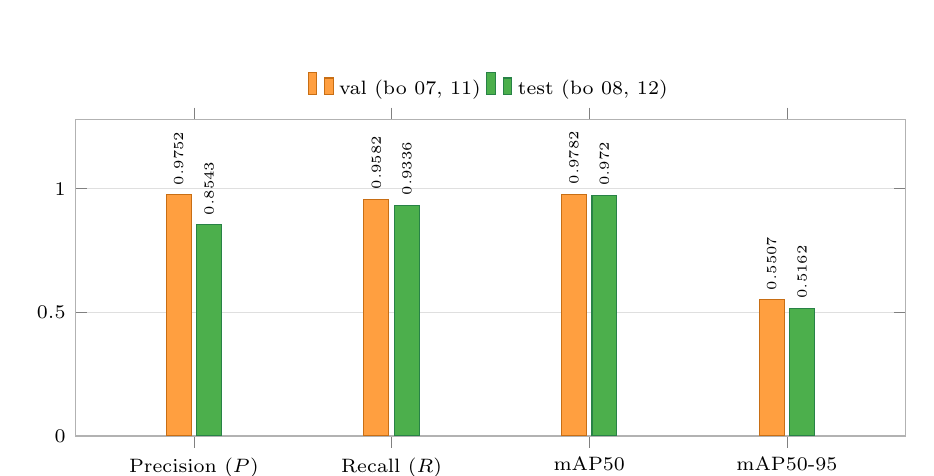
\begin{tikzpicture}
\begin{axis}[bieudo,height=5.6cm,ymax=1.28,
  symbolic x coords={P,R,mAP50,mAP50-95},xtick=data,
  xticklabels={Precision ($P$),Recall ($R$),mAP50,mAP50-95}]
\addplot[fill=orange!75,draw=camdam] coordinates {(P,0.9752)(R,0.9582)(mAP50,0.9782)(mAP50-95,0.5507)};
\addplot[fill=green!55!black!70,draw=luc] coordinates {(P,0.8543)(R,0.9336)(mAP50,0.9720)(mAP50-95,0.5162)};
\legend{{val (bo 07, 11)},{test (bo 08, 12)}}
\end{axis}
\end{tikzpicture}
\caption{YOLOv8s (\texttt{pcb\_v8s\_board}) trên val và test. Precision giảm từ $0.9752$ xuống $0.8543$ khi gặp bo chưa từng thấy.}
\label{fig:valtest}
\end{figure}

\needspace{24\baselineskip}
\muc{5.3. Đường SIFT + XOR}

Khớp box nhãn và box dự đoán theo IoU, tham lam theo IoU giảm dần, mỗi box dùng tối đa một lần, \textbf{không xét lớp} (chỉ đánh giá khả năng tìm vùng lỗi).
\begin{table}[H]
\centering
\small
\caption{Đường SIFT + XOR theo ngưỡng IoU (không xét lớp)}\label{tab:xoriou}
\begin{tabular}{l|l|c|rr|ccc}
\toprule
\textbf{Tập} & \textbf{Bản} & \textbf{IoU} & \textbf{Box dự đoán} & \textbf{TP} & $P$ & $R$ & $F1$ \\ \midrule
val & \texttt{orig} & 0.5 & 2273 & 0 & 0.0000 & 0.0000 & 0.0000 \\
val & \texttt{orig} & 0.3 & 2273 & 15 & 0.0066 & 0.0249 & 0.0104 \\
val & \texttt{orig} & 0.1 & 2273 & 216 & 0.0950 & 0.3582 & 0.1502 \\
val & \texttt{new} & 0.5 & 598 & 371 & 0.6204 & 0.6153 & 0.6178 \\
val & \texttt{new} & 0.3 & 598 & 571 & 0.9548 & 0.9469 & 0.9509 \\
val & \texttt{new} & 0.1 & 598 & 596 & 0.9967 & 0.9884 & 0.9925 \\ \midrule
test & \texttt{orig} & 0.5 & 2180 & 1 & 0.0005 & 0.0017 & 0.0007 \\
test & \texttt{orig} & 0.3 & 2180 & 14 & 0.0064 & 0.0233 & 0.0101 \\
test & \texttt{orig} & 0.1 & 2180 & 258 & 0.1183 & 0.4293 & 0.1855 \\
test & \texttt{new} & 0.5 & 569 & 373 & 0.6555 & 0.6206 & 0.6376 \\
test & \texttt{new} & 0.3 & 569 & 553 & 0.9719 & 0.9201 & 0.9453 \\
test & \texttt{new} & 0.1 & 569 & 558 & 0.9807 & 0.9285 & 0.9538 \\ \bottomrule
\end{tabular}
\end{table}
\begin{itemize}
  \item \textbf{Bản gốc} sinh 2273 (val) và 2180 (test) box cho khoảng 600 nhãn, F1 ở IoU $0.5$ gần bằng 0 (test: 1 TP).
  \item \textbf{Bản cải tiến} giảm còn 598 (val) và 569 (test) box; F1 ở IoU $0.5$ là $0.6178$ (val) và $0.6376$ (test).
  \item Ở IoU thấp hơn, F1 rất cao ($0.9453$ ở IoU $0.3$ và $0.9538$ ở IoU $0.1$ trên test). Vùng lỗi phần lớn được tìm đúng chỗ; điểm thấp ở IoU $0.5$ đến từ độ khớp giữa box XOR và box nhãn.
\end{itemize}

\hinhref{f1iou} so hai bản của đường XOR theo ngưỡng IoU (số liệu ở \bangref{xoriou}): bản cải tiến vượt xa bản gốc ở mọi ngưỡng, và điểm tụt ở IoU $0.5$ là do độ khớp box chứ không phải do không tìm ra vùng lỗi.

\begin{figure}[H]
\centering
\begin{subfigure}[t]{0.49\linewidth}
\centering
\begin{tikzpicture}
\begin{axis}[bieudo,width=\linewidth,height=5.2cm,ymax=1.3,bar width=11pt,
  symbolic x coords={i1,i3,i5},xtick=data,xticklabels={0.1,0.3,0.5},xlabel={Ngưỡng IoU},ylabel={F1},
  /pgf/number format/precision=3]
\addplot[fill=gray!55,draw=gray!70!black] coordinates {(i1,0.1502)(i3,0.0104)(i5,0.0000)};
\addplot[fill=blue!45!black!70,draw=chinh] coordinates {(i1,0.9925)(i3,0.9509)(i5,0.6178)};
\legend{\texttt{orig},\texttt{new}}
\end{axis}
\end{tikzpicture}
\subcaption{Val}
\end{subfigure}\hfill
\begin{subfigure}[t]{0.49\linewidth}
\centering
\begin{tikzpicture}
\begin{axis}[bieudo,width=\linewidth,height=5.2cm,ymax=1.3,bar width=11pt,
  symbolic x coords={i1,i3,i5},xtick=data,xticklabels={0.1,0.3,0.5},xlabel={Ngưỡng IoU},ylabel={F1},
  /pgf/number format/precision=3]
\addplot[fill=gray!55,draw=gray!70!black] coordinates {(i1,0.1855)(i3,0.0101)(i5,0.0007)};
\addplot[fill=blue!45!black!70,draw=chinh] coordinates {(i1,0.9538)(i3,0.9453)(i5,0.6376)};
\legend{\texttt{orig},\texttt{new}}
\end{axis}
\end{tikzpicture}
\subcaption{Test}
\end{subfigure}
\caption{F1 của đường SIFT + XOR (không xét lớp) theo ngưỡng IoU: bản gốc (\texttt{orig}) và bản cải tiến (\texttt{new}).}
\label{fig:f1iou}
\end{figure}

\muc{5.4. Bộ phân loại ảnh cắt}

\begin{itemize}
  \item \textbf{Trên ảnh cắt theo nhãn thật} (cận trên, vì ảnh cắt đúng vị trí nhãn): top-1 val $1.000$, test $0.990$ ($595/601$). Sáu ảnh sai trên test: 5 ảnh Spur nhận thành Spurious Copper, 1 ảnh Mouse Bite nhận thành Open Circuit.
  \item \textbf{Trên box do đường XOR tìm được} (IoU $\ge 0.5$ với nhãn): val $0.9973$ ($n=371$), test $0.9169$ ($342/373$).
\end{itemize}

\needspace{12\baselineskip}
\begin{table}[H]
\centering
\small
\caption{Ma trận nhầm lẫn của bộ phân loại ảnh cắt trên test (box tìm bởi XOR; hàng: lớp thật, cột: lớp dự đoán)}\label{tab:nhamlan}
\begin{tabular}{l|cccccc|c}
\toprule
 & MH & MB & OC & SH & SP & SC & \textbf{Tổng} \\ \midrule
Missing Hole (MH) & 33 & 0 & 0 & 0 & 0 & 0 & 33 \\
Mouse Bite (MB) & 0 & 86 & 1 & 0 & 0 & 0 & 87 \\
Open Circuit (OC) & 0 & 0 & 86 & 0 & 0 & 0 & 86 \\
Short (SH) & 0 & 0 & 0 & 62 & 0 & 2 & 64 \\
Spur (SP) & 0 & 0 & 0 & 0 & 19 & 28 & 47 \\
Spurious Copper (SC) & 0 & 0 & 0 & 0 & 0 & 56 & 56 \\ \bottomrule
\end{tabular}
\end{table}
\begin{itemize}
  \item Điểm yếu rõ nhất là \textbf{Spur bị nhận thành Spurious Copper}: $28/47$ box Spur sai trên test. Cặp này cũng là nguồn lỗi chính khi phân loại ảnh cắt theo nhãn thật (5/6 ảnh sai).
  \item Các lớp còn lại đều đạt từ $0.969$ trở lên trên test.
  \item Trên val chỉ có 1 box sai (Spurious Copper nhận thành Mouse Bite).
\end{itemize}

\hinhref{nhamlan} vẽ lại ma trận ở \bangref{nhamlan} bằng màu: ô càng đậm thì tỉ lệ của lớp thật càng cao (chuẩn hoá theo hàng). Ô lệch đường chéo đáng kể duy nhất là Spur nhận thành Spurious Copper.

\begin{figure}[H]
\centering
\begin{tikzpicture}[x=1cm,y=1cm]
\node[minimum width=1.12cm,minimum height=0.86cm,fill=chinh!100!white,draw=white,line width=1pt,text=white,font=\small] at (0.00,0.00) {33};
\node[minimum width=1.12cm,minimum height=0.86cm,fill=chinh!0!white,draw=white,line width=1pt,text=black,font=\small] at (1.12,0.00) {0};
\node[minimum width=1.12cm,minimum height=0.86cm,fill=chinh!0!white,draw=white,line width=1pt,text=black,font=\small] at (2.24,0.00) {0};
\node[minimum width=1.12cm,minimum height=0.86cm,fill=chinh!0!white,draw=white,line width=1pt,text=black,font=\small] at (3.36,0.00) {0};
\node[minimum width=1.12cm,minimum height=0.86cm,fill=chinh!0!white,draw=white,line width=1pt,text=black,font=\small] at (4.48,0.00) {0};
\node[minimum width=1.12cm,minimum height=0.86cm,fill=chinh!0!white,draw=white,line width=1pt,text=black,font=\small] at (5.60,0.00) {0};
\node[font=\scriptsize,anchor=east] at (-0.7,0.00) {Missing Hole};
\node[font=\small\bfseries,anchor=west] at (6.30,0.00) {33};
\node[minimum width=1.12cm,minimum height=0.86cm,fill=chinh!0!white,draw=white,line width=1pt,text=black,font=\small] at (0.00,-0.86) {0};
\node[minimum width=1.12cm,minimum height=0.86cm,fill=chinh!99!white,draw=white,line width=1pt,text=white,font=\small] at (1.12,-0.86) {86};
\node[minimum width=1.12cm,minimum height=0.86cm,fill=chinh!1!white,draw=white,line width=1pt,text=black,font=\small] at (2.24,-0.86) {1};
\node[minimum width=1.12cm,minimum height=0.86cm,fill=chinh!0!white,draw=white,line width=1pt,text=black,font=\small] at (3.36,-0.86) {0};
\node[minimum width=1.12cm,minimum height=0.86cm,fill=chinh!0!white,draw=white,line width=1pt,text=black,font=\small] at (4.48,-0.86) {0};
\node[minimum width=1.12cm,minimum height=0.86cm,fill=chinh!0!white,draw=white,line width=1pt,text=black,font=\small] at (5.60,-0.86) {0};
\node[font=\scriptsize,anchor=east] at (-0.7,-0.86) {Mouse Bite};
\node[font=\small\bfseries,anchor=west] at (6.30,-0.86) {87};
\node[minimum width=1.12cm,minimum height=0.86cm,fill=chinh!0!white,draw=white,line width=1pt,text=black,font=\small] at (0.00,-1.72) {0};
\node[minimum width=1.12cm,minimum height=0.86cm,fill=chinh!0!white,draw=white,line width=1pt,text=black,font=\small] at (1.12,-1.72) {0};
\node[minimum width=1.12cm,minimum height=0.86cm,fill=chinh!100!white,draw=white,line width=1pt,text=white,font=\small] at (2.24,-1.72) {86};
\node[minimum width=1.12cm,minimum height=0.86cm,fill=chinh!0!white,draw=white,line width=1pt,text=black,font=\small] at (3.36,-1.72) {0};
\node[minimum width=1.12cm,minimum height=0.86cm,fill=chinh!0!white,draw=white,line width=1pt,text=black,font=\small] at (4.48,-1.72) {0};
\node[minimum width=1.12cm,minimum height=0.86cm,fill=chinh!0!white,draw=white,line width=1pt,text=black,font=\small] at (5.60,-1.72) {0};
\node[font=\scriptsize,anchor=east] at (-0.7,-1.72) {Open Circuit};
\node[font=\small\bfseries,anchor=west] at (6.30,-1.72) {86};
\node[minimum width=1.12cm,minimum height=0.86cm,fill=chinh!0!white,draw=white,line width=1pt,text=black,font=\small] at (0.00,-2.58) {0};
\node[minimum width=1.12cm,minimum height=0.86cm,fill=chinh!0!white,draw=white,line width=1pt,text=black,font=\small] at (1.12,-2.58) {0};
\node[minimum width=1.12cm,minimum height=0.86cm,fill=chinh!0!white,draw=white,line width=1pt,text=black,font=\small] at (2.24,-2.58) {0};
\node[minimum width=1.12cm,minimum height=0.86cm,fill=chinh!97!white,draw=white,line width=1pt,text=white,font=\small] at (3.36,-2.58) {62};
\node[minimum width=1.12cm,minimum height=0.86cm,fill=chinh!0!white,draw=white,line width=1pt,text=black,font=\small] at (4.48,-2.58) {0};
\node[minimum width=1.12cm,minimum height=0.86cm,fill=chinh!3!white,draw=white,line width=1pt,text=black,font=\small] at (5.60,-2.58) {2};
\node[font=\scriptsize,anchor=east] at (-0.7,-2.58) {Short};
\node[font=\small\bfseries,anchor=west] at (6.30,-2.58) {64};
\node[minimum width=1.12cm,minimum height=0.86cm,fill=chinh!0!white,draw=white,line width=1pt,text=black,font=\small] at (0.00,-3.44) {0};
\node[minimum width=1.12cm,minimum height=0.86cm,fill=chinh!0!white,draw=white,line width=1pt,text=black,font=\small] at (1.12,-3.44) {0};
\node[minimum width=1.12cm,minimum height=0.86cm,fill=chinh!0!white,draw=white,line width=1pt,text=black,font=\small] at (2.24,-3.44) {0};
\node[minimum width=1.12cm,minimum height=0.86cm,fill=chinh!0!white,draw=white,line width=1pt,text=black,font=\small] at (3.36,-3.44) {0};
\node[minimum width=1.12cm,minimum height=0.86cm,fill=chinh!40!white,draw=white,line width=1pt,text=black,font=\small] at (4.48,-3.44) {19};
\node[minimum width=1.12cm,minimum height=0.86cm,fill=chinh!60!white,draw=white,line width=1pt,text=white,font=\small] at (5.60,-3.44) {28};
\node[font=\scriptsize,anchor=east] at (-0.7,-3.44) {Spur};
\node[font=\small\bfseries,anchor=west] at (6.30,-3.44) {47};
\node[minimum width=1.12cm,minimum height=0.86cm,fill=chinh!0!white,draw=white,line width=1pt,text=black,font=\small] at (0.00,-4.30) {0};
\node[minimum width=1.12cm,minimum height=0.86cm,fill=chinh!0!white,draw=white,line width=1pt,text=black,font=\small] at (1.12,-4.30) {0};
\node[minimum width=1.12cm,minimum height=0.86cm,fill=chinh!0!white,draw=white,line width=1pt,text=black,font=\small] at (2.24,-4.30) {0};
\node[minimum width=1.12cm,minimum height=0.86cm,fill=chinh!0!white,draw=white,line width=1pt,text=black,font=\small] at (3.36,-4.30) {0};
\node[minimum width=1.12cm,minimum height=0.86cm,fill=chinh!0!white,draw=white,line width=1pt,text=black,font=\small] at (4.48,-4.30) {0};
\node[minimum width=1.12cm,minimum height=0.86cm,fill=chinh!100!white,draw=white,line width=1pt,text=white,font=\small] at (5.60,-4.30) {56};
\node[font=\scriptsize,anchor=east] at (-0.7,-4.30) {Spurious Copper};
\node[font=\small\bfseries,anchor=west] at (6.30,-4.30) {56};
\node[font=\scriptsize] at (0.00,0.7) {MH};
\node[font=\scriptsize] at (1.12,0.7) {MB};
\node[font=\scriptsize] at (2.24,0.7) {OC};
\node[font=\scriptsize] at (3.36,0.7) {SH};
\node[font=\scriptsize] at (4.48,0.7) {SP};
\node[font=\scriptsize] at (5.60,0.7) {SC};
\node[font=\scriptsize\bfseries] at (2.8,1.15) {Lớp dự đoán};
\node[font=\scriptsize\bfseries,rotate=90] at (-3.5,-2.15) {Lớp thật};
\node[font=\scriptsize\bfseries,anchor=west] at (6.3,0.7) {Tổng};
\end{tikzpicture}
\caption{Ma trận nhầm lẫn của bộ phân loại ảnh cắt trên các box do đường XOR tìm được (test, $n=373$); số trong ô là số box, màu theo tỉ lệ trong hàng.}
\label{fig:nhamlan}
\end{figure}

\muc{5.5. Kết quả theo lớp và ma trận nhầm lẫn của YOLOv8s trên test}

\bangref{theolop} liệt kê $P$, $R$, AP50 và AP50-95 của từng lớp trên test.

\begin{table}[H]
\centering
\small
\caption{$P$, $R$, AP50 và AP50-95 theo lớp của YOLOv8s trên test (\texttt{results/pcb\_v8s\_board\_test/metrics\_per\_class.csv})}\label{tab:theolop}
\begin{tabular}{l|r|cccc}
\toprule
\textbf{Lớp} & \textbf{Số box} & $P$ & $R$ & AP50 & AP50-95 \\ \midrule
Missing Hole & 101 & 0.6272 & 0.9802 & 0.9879 & 0.6364 \\
Mouse Bite & 100 & 0.9509 & 0.9678 & 0.9777 & 0.4758 \\
Open Circuit & 100 & 0.9834 & 0.9600 & 0.9830 & 0.4932 \\
Short & 99 & 0.6130 & 0.9899 & 0.9813 & 0.4803 \\
Spur & 101 & 1.0000 & 0.7138 & 0.9312 & 0.5221 \\
Spurious Copper & 100 & 0.9514 & 0.9900 & 0.9705 & 0.4896 \\ \midrule
\textbf{Tất cả} & \textbf{601} & \textbf{0.8543} & \textbf{0.9336} & \textbf{0.9720} & \textbf{0.5162} \\ \bottomrule
\end{tabular}
\end{table}
\begin{itemize}
  \item $P$ và $R$ do Ultralytics tính tại độ tin cậy cho F1 cao nhất của đường cong F1 (khoảng $0.471$), nên khác các số theo conf của Mục 6.5 và 7.3. Dòng cuối trùng với Mục 5.2.
  \item AP50 đều cao ($0.9312$ đến $0.9879$), nhưng \textbf{precision thấp ở Missing Hole ($0.6272$) và Short ($0.6130$)}, khớp với box thừa ở Mục 6.3.
  \item \textbf{Spur} có $P=1.0000$ nhưng recall thấp nhất ($0.7138$). AP50-95 thấp nhất ở Mouse Bite ($0.4758$), cao nhất ở Missing Hole ($0.6364$).
\end{itemize}

\hinhref{nhamlan_yolo} là ma trận nhầm lẫn chuẩn hoá theo cột (lớp thật). Các lớp đều đạt từ $0.99$ trở lên, riêng Spur $0.89$; nhầm lẫn đáng kể duy nhất là Spur bị dự đoán thành Spurious Copper ($6$ box, $0.06$).

\begin{figure}[H]
\centering
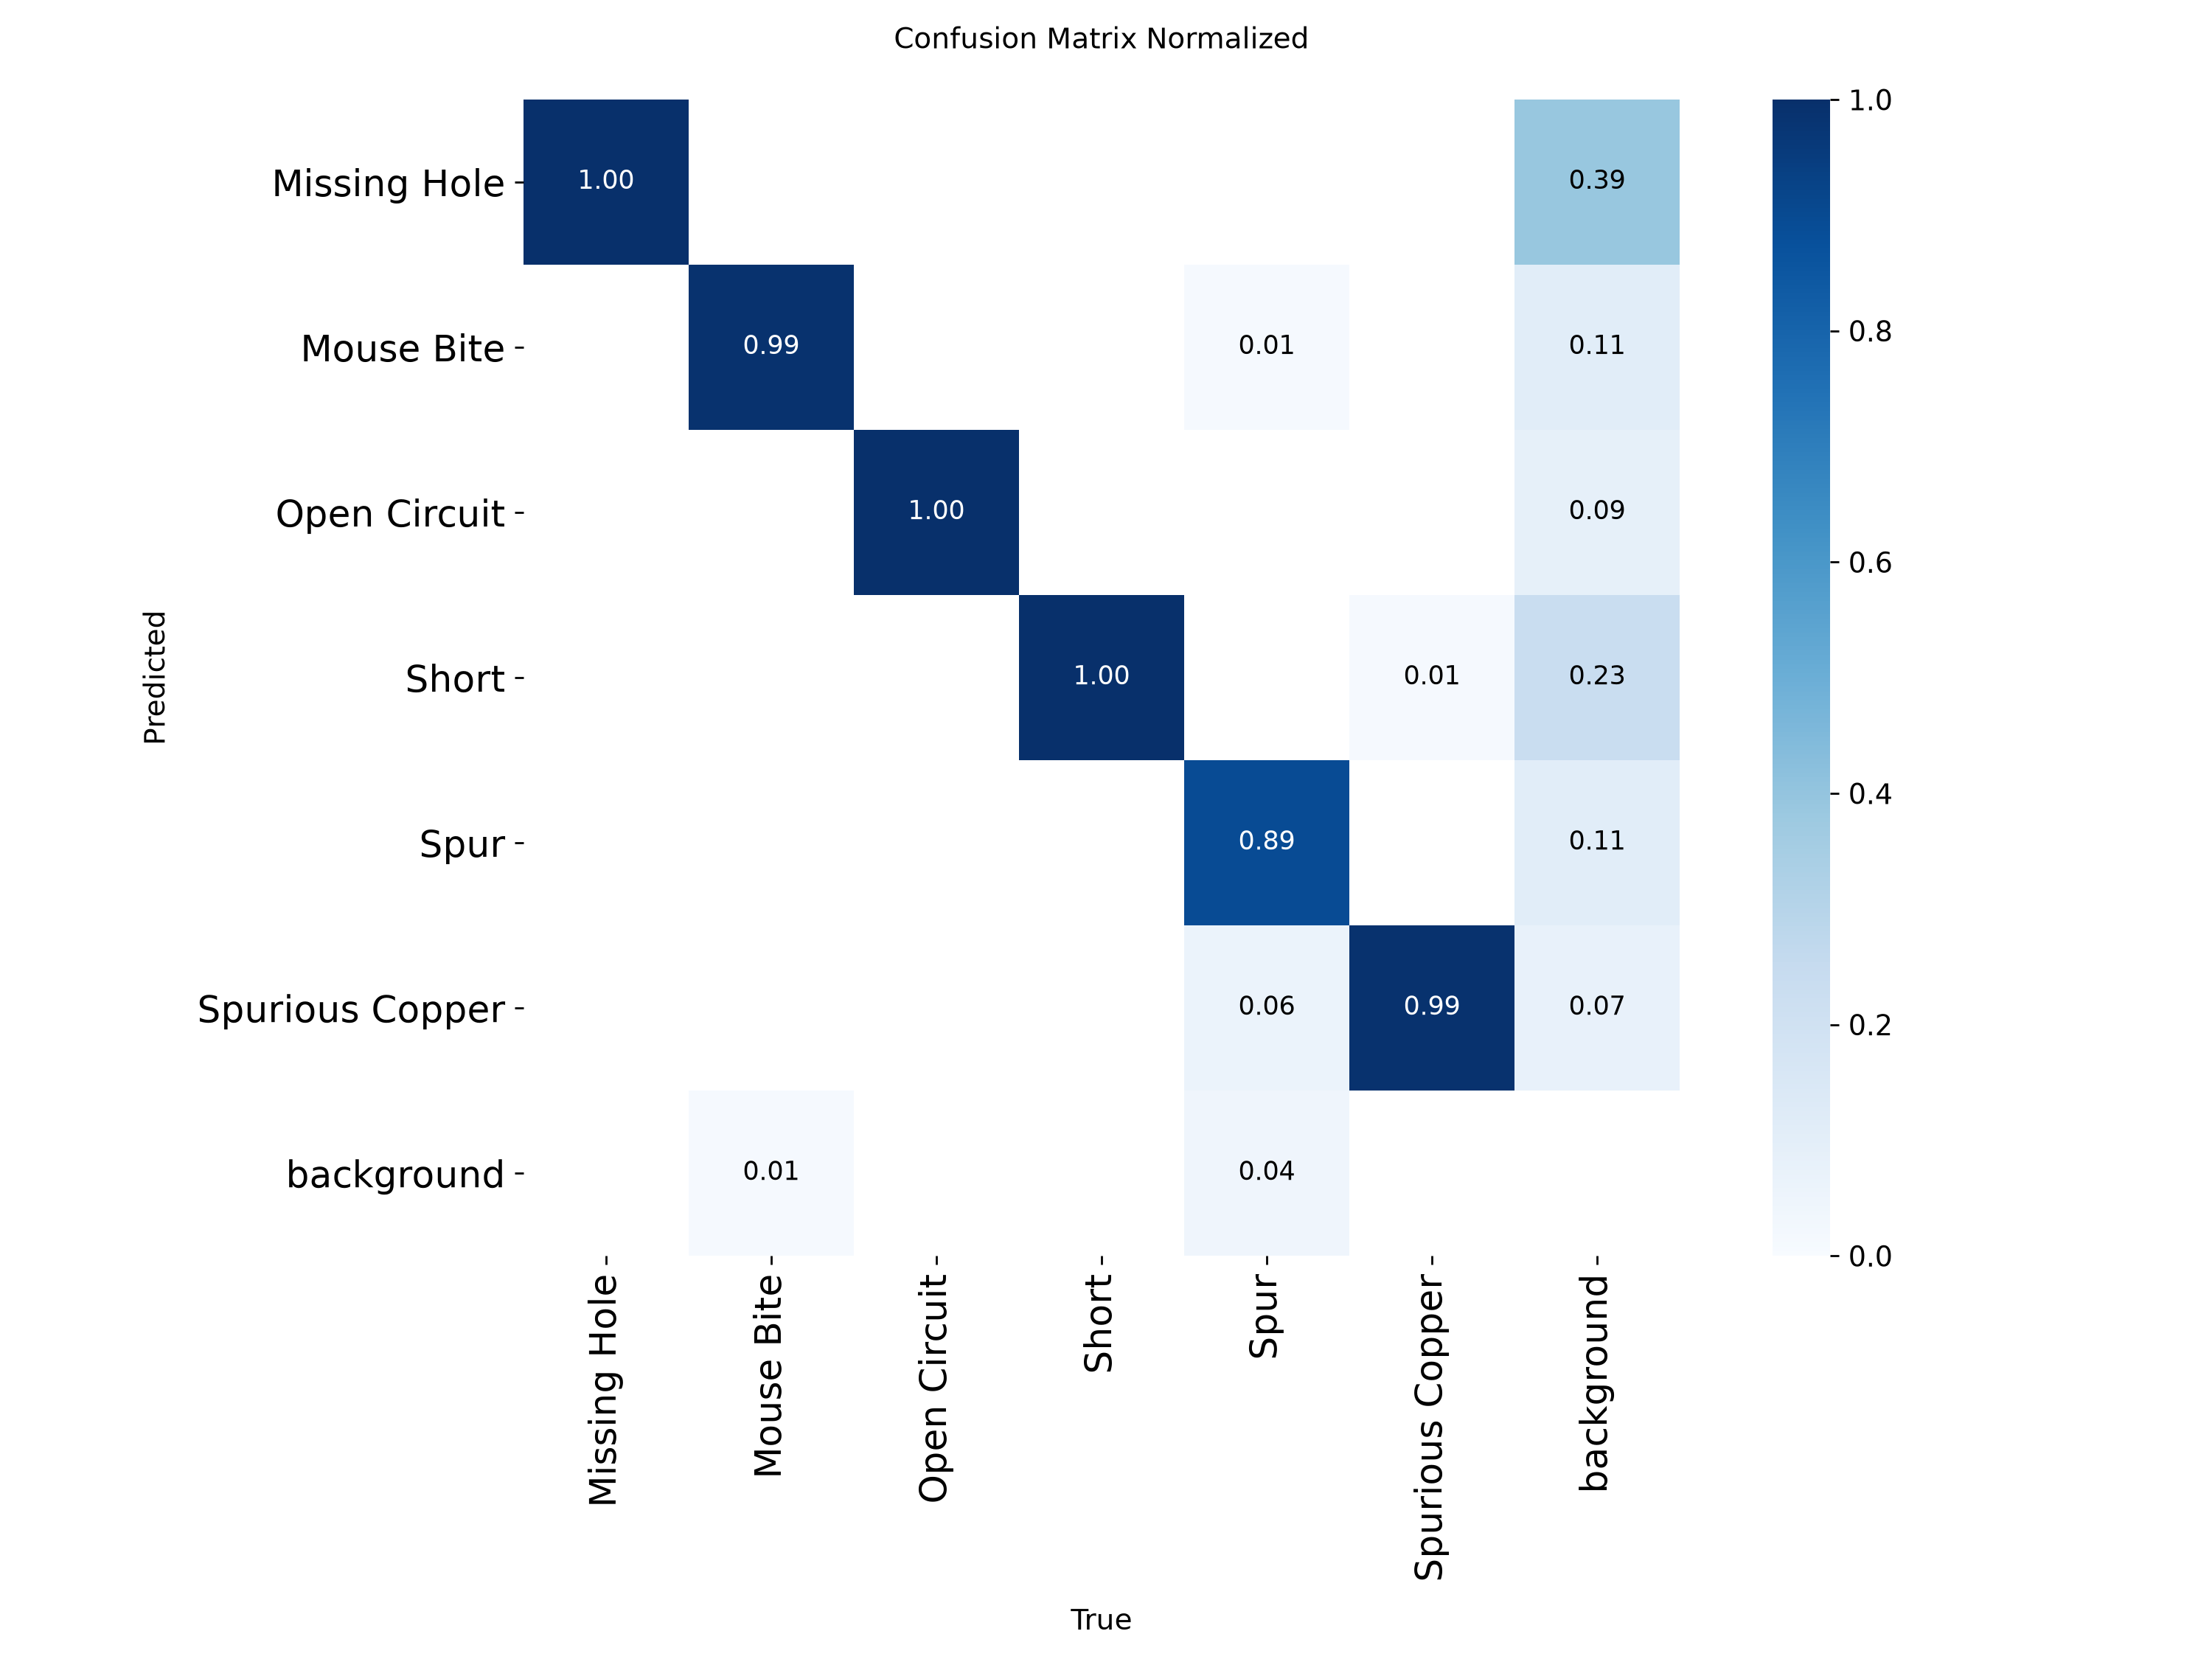
\includegraphics[width=0.8\textwidth]{pcb_v8s_board_test/confusion_matrix_normalized.png}
\caption{Ma trận nhầm lẫn chuẩn hoá của YOLOv8s trên test (do Ultralytics sinh). Hàng: lớp dự đoán; cột: lớp thật. Cột \emph{background}: box dự đoán không ứng với nhãn nào (báo thừa); hàng \emph{background}: nhãn bị bỏ sót.}
\label{fig:nhamlan_yolo}
\end{figure}

\muc{5.6. Độ bền với xoay, nghiêng, mờ và thiếu sáng}

Dữ liệu huấn luyện là ảnh chụp thẳng, đủ sáng; ảnh thực tế có thể xoay, nghiêng, nhòe hoặc tối. Mục này đo mô hình trên chính các ảnh của tập đánh giá sau khi biến đổi. \texttt{tools/perturb.py} tạo các biến đổi (không ngẫu nhiên, nên chạy lại ra đúng ảnh cũ) và \texttt{tools/eval\_robustness.py} chạy Ultralytics trên từng mức, ghi \texttt{results/robustness.csv}.

\begin{itemize}
  \item \textbf{Xoay:} $90^\circ$ và $180^\circ$ chính xác từng pixel; $15^\circ$ và $45^\circ$ xoay quanh tâm, mở rộng khung để không mất nội dung.
  \item \textbf{Nghiêng:} biến đổi phối cảnh, cạnh trên thu hẹp $5\%$, $10\%$ và $15\%$ bề rộng ở mỗi bên.
  \item \textbf{Mờ và tối:} Gaussian blur $\sigma = 1, 2, 3, 5$ pixel của ảnh gốc, motion blur dài $15$ pixel; giảm sáng bằng cách nhân cường độ với $0.5$.
  \item \textbf{Nhãn:} bốn góc của box được biến đổi theo ảnh rồi lấy hộp bao; với mờ và tối, box giữ nguyên.
\end{itemize}

\textbf{Hạn chế của phép đo.} Với box nhỏ, xoay $45^\circ$ làm hộp bao nở khoảng gấp đôi diện tích (cột \emph{độ khít nhãn} trong \bangref{chiunhieu_test}). IoU giữa box khít vào lỗi và nhãn bị nở bị chặn trên, nên mAP50 ở mức xoay góc lẻ và nghiêng phản ánh cả độ khít của nhãn chứ không chỉ chất lượng mô hình. Gaussian blur tính $\sigma$ theo pixel của ảnh gốc, trước khi ảnh được thu về \texttt{imgsz}, nên cùng một $\sigma$ nhẹ hơn khi nhìn ở độ phân giải huấn luyện.

\textbf{Augmentation chịu nhiễu.} Bản huấn luyện thêm augmentation dùng \texttt{configs/aug\_robust.yaml}: lật ngang và dọc, xoay bội $90^\circ$, xoay góc nhỏ $\pm 10^\circ$, perspective nhỏ, blur, median blur, motion blur và giảm sáng. Không xoay góc lớn tự do vì box của lỗi nhỏ sẽ nở ra khi xoay, làm nhãn kém chính xác.

\IfFileExists{bang_chiunhieu_test.tex}{%
  \begin{table}[H]
\centering
\small
\caption{Độ bền theo điều kiện nhiễu, tập test (\texttt{results/robustness.csv}). Độ khít nhãn là tỉ lệ diện tích box gốc so với box sau biến đổi; dưới 1 nghĩa là nhãn bị nở ra nên mAP50 bị chặn trên.}\label{tab:chiunhieu_test}
\begin{tabular}{l|c|cc|cc}
\toprule
\textbf{Điều kiện} & \textbf{Độ khít nhãn} & \multicolumn{2}{c}{\texttt{pcb\_final\_aug}} & \multicolumn{2}{c}{\texttt{pcb\_v8s\_board}} \\
 &  & mAP50 & $R$ & mAP50 & $R$ \\ \midrule
Gốc & 1.00 & 0.9730 & 0.9305 & 0.9720 & 0.9336 \\
Xoay 15° & 0.65 & 0.9480 & 0.9133 & 0.5776 & 0.5575 \\
Xoay 45° & 0.48 & 0.6090 & 0.6498 & 0.4138 & 0.4990 \\
Xoay 90° & 1.00 & 0.9126 & 0.9502 & 0.9563 & 0.9507 \\
Xoay 180° & 1.00 & 0.9280 & 0.9521 & 0.9427 & 0.8853 \\
Nghiêng 5\% & 0.98 & 0.9271 & 0.9305 & 0.9675 & 0.9043 \\
Nghiêng 10\% & 0.96 & 0.9693 & 0.8664 & 0.9101 & 0.9024 \\
Nghiêng 15\% & 0.95 & 0.9152 & 0.9432 & 0.8197 & 0.8626 \\
Blur σ=1 & 1.00 & 0.9766 & 0.9360 & 0.9752 & 0.9346 \\
Blur σ=2 & 1.00 & 0.9466 & 0.9675 & 0.9574 & 0.8762 \\
Blur σ=3 & 1.00 & 0.9152 & 0.9709 & 0.9270 & 0.8834 \\
Blur σ=5 & 1.00 & 0.9023 & 0.9657 & 0.7809 & 0.7127 \\
Motion blur 15 px & 1.00 & 0.9472 & 0.8549 & 0.9166 & 0.8296 \\
Tối 50\% & 1.00 & 0.9216 & 0.9503 & 0.9446 & 0.8934 \\
\bottomrule
\end{tabular}
\end{table}

  \begin{figure}[H]
  \centering
  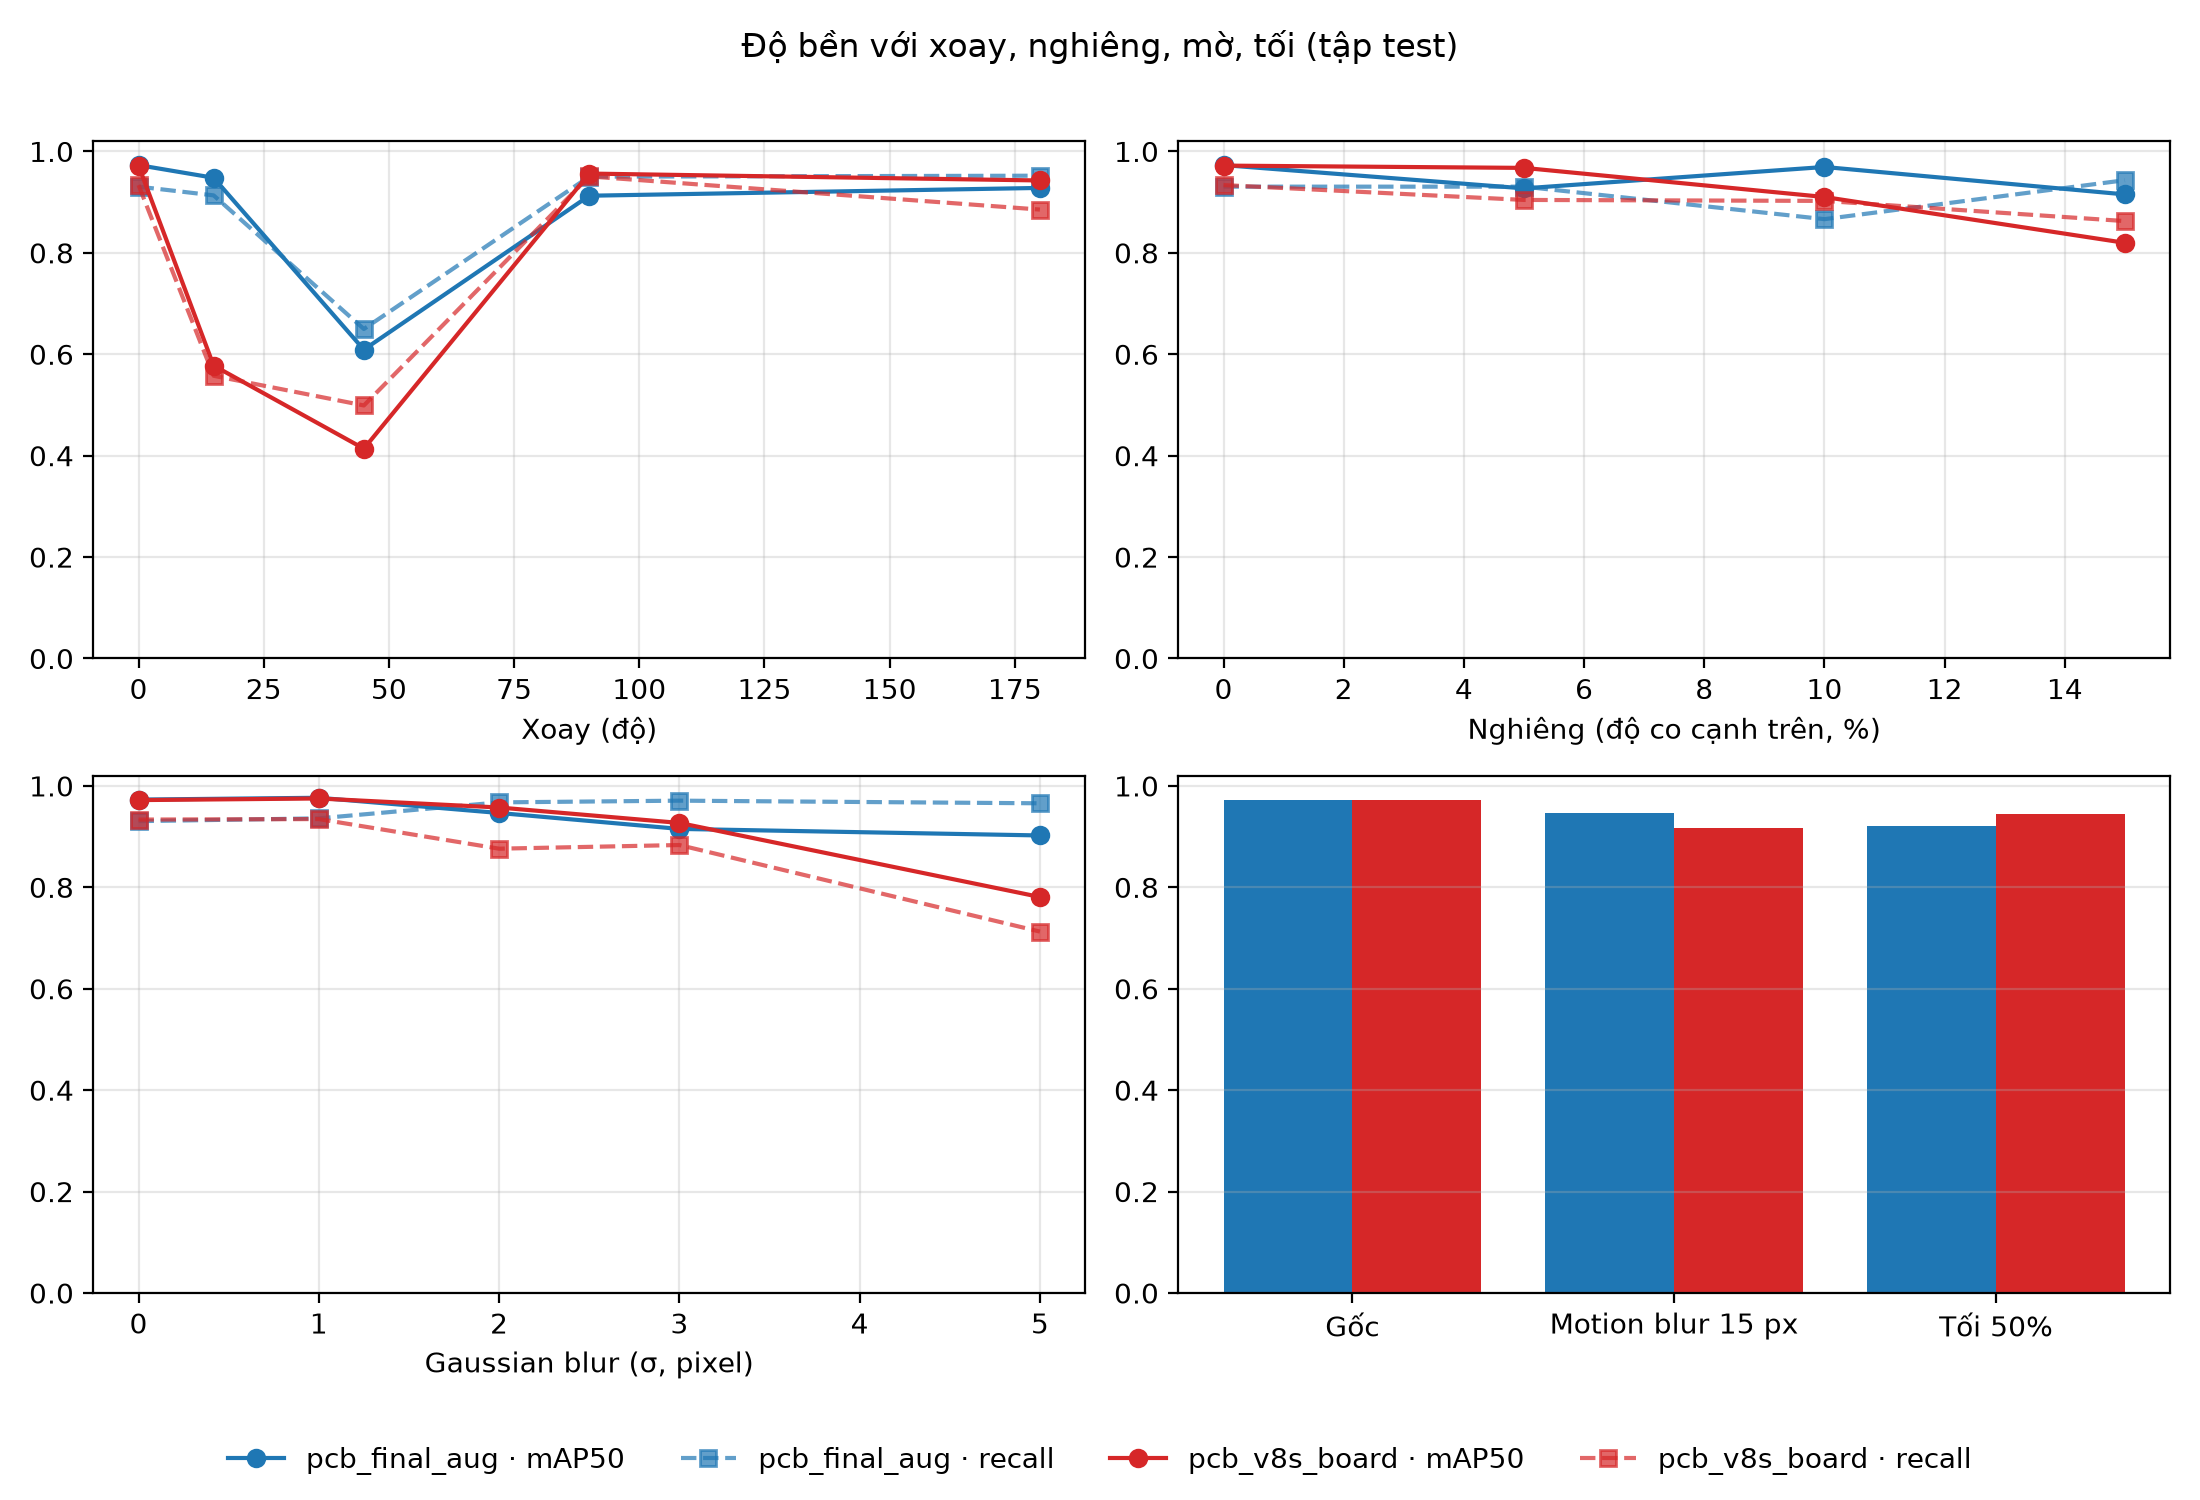
\includegraphics[width=\textwidth]{robustness_test.png}
  \caption{Đường cong mAP50 và recall theo mức xoay, nghiêng, mờ, tối trên tập test (vẽ từ \texttt{results/robustness.csv} bằng \texttt{tools/plot\_robustness.py}).}
  \label{fig:chiunhieu_test}
  \end{figure}
  % TODO sau khi có số liệu: viết 2-3 gạch đầu dòng nhận xét (mức nào mô hình cũ tụt, mô hình có augmentation hơn bao nhiêu, mức nào không hơn).
}{%
  \par\textcolor{red}{\textbf{CHƯA CÓ SỐ LIỆU:} chạy \texttt{tools/eval\_robustness.py} và \texttt{tools/plot\_robustness.py --split test} để sinh bảng và hình cho mục này.}\par
}

%=====================================================================
\chuong{CHƯƠNG 6: PHÂN TÍCH LỖI CỦA BỘ PHÁT HIỆN}
\sochuong{6}
%=====================================================================

\muc{6.1. Cách phân loại lỗi}

Dùng \texttt{tools/analyze\_errors.py}, \texttt{imgsz} 1024, độ tin cậy (conf) $0.25$.
\begin{itemize}
  \item Ghép 1--1 box dự đoán với nhãn theo độ tin cậy giảm dần, IoU $\ge 0.5$, không xét lớp.
  \item \textbf{Đúng:} ghép được và cùng lớp. \textbf{Nhầm lớp:} ghép được nhưng khác lớp. \textbf{Bỏ sót:} nhãn không được ghép. \textbf{Báo thừa:} box dự đoán không được ghép.
  \item Box thừa chia thêm ba loại theo IoU lớn nhất với nhãn: \emph{trùng} ($\ge 0.5$, nhãn đó đã được ghép với box khác), \emph{lệch} ($0.1$ đến dưới $0.5$), \emph{nền} (dưới $0.1$).
\end{itemize}

Quy tắc phân loại trên được tóm tắt thành lưu đồ ở \hinhref{phanloailoi}.

\begin{figure}[H]
\centering
\begin{tikzpicture}[x=1cm,y=1cm,scale=0.9,transform shape]
\tikzset{nhan/.append style={font=\scriptsize\itshape}}
\node[khoi vao,text width=30mm] (s) at (0,0) {Với mỗi box dự đoán\\(độ tin cậy giảm dần)};
\node[quyet,text width=31mm] (q1) at (5.7,0) {Ghép được với\\nhãn chưa dùng,\\IoU $\ge0.5$?};
\node[quyet,text width=22mm] (q2) at (10.8,0) {Cùng\\lớp?};
\node[khoi ra,text width=22mm] (tp) at (14.7,0.95) {\textbf{Đúng}};
\node[khoi do,text width=22mm] (cf) at (14.7,-0.95) {\textbf{Nhầm lớp}};
\node[khoi do,text width=30mm] (fp) at (5.7,-2.7) {\textbf{Báo thừa}\\(không ghép được)};
\draw[mui] (s)--(q1);
\draw[mui] (q1)--node[above,nhan]{có}(q2);
\draw[mui] (q2.north east)--++(0.5,0)|-(tp.west) node[pos=0.7,above,nhan]{có};
\draw[mui] (q2.south east)--++(0.5,0)|-(cf.west) node[pos=0.7,below,nhan]{không};
\draw[mui] (q1.south)--node[right,nhan]{không}(fp);
% ba loại box thừa
\node[khoi,text width=22mm,fill=red!4] (f1) at (1.0,-5.2) {\textbf{Trùng}\\IoU lớn nhất $\ge0.5$ (nhãn đã được ghép)};
\node[khoi,text width=22mm,fill=red!4] (f2) at (5.7,-5.2) {\textbf{Lệch}\\IoU lớn nhất từ $0.1$ đến dưới $0.5$};
\node[khoi,text width=22mm,fill=red!4] (f3) at (10.4,-5.2) {\textbf{Nền}\\IoU lớn nhất dưới $0.1$};
\draw[mui] (fp.south) -- ++(0,-0.35) -| (f1.north);
\draw[mui] (fp.south) -- (f2.north);
\draw[mui] (fp.south) -- ++(0,-0.35) -| (f3.north);
\node[khoi do,text width=22mm] (fn) at (14.7,-5.2) {\textbf{Bỏ sót}\\nhãn không được ghép};
\end{tikzpicture}
\caption{Phân loại kết quả của bộ phát hiện (Mục 6.1). Box thừa chia thêm theo IoU lớn nhất với nhãn.}
\label{fig:phanloailoi}
\end{figure}

\muc{6.2. Lỗi trên val}

\begin{table}[H]
\centering
\small
\caption{Phân loại kết quả của bộ phát hiện trên val (conf $0.25$)}\label{tab:loival}
\begin{tabular}{l|rrrrr}
\toprule
\textbf{Mô hình (chia theo bo)} & \textbf{Nhãn} & \textbf{Đúng} & \textbf{Nhầm lớp} & \textbf{Bỏ sót} & \textbf{Báo thừa} \\ \midrule
\texttt{pcb\_v8s\_board} & 603 & 589 & 3 & 11 & 20 \\
\texttt{pcb\_v8n\_board} & 603 & 566 & 11 & 26 & 28 \\ \bottomrule
\end{tabular}
\end{table}
\begin{itemize}
  \item v8s đúng $589/603$ ($97.7\%$), v8n đúng $566/603$ ($93.9\%$).
  \item v8s ít hơn v8n ở cả ba loại lỗi. Đây là cơ sở chọn v8s ở Mục 5.1.
\end{itemize}

\hinhref{loival} vẽ lại \bangref{loival}: v8s ít box sai hơn v8n ở cả ba loại.

\begin{figure}[H]
\centering
\begin{tikzpicture}
\begin{axis}[bieudo,height=5.2cm,width=0.82\linewidth,ymax=34,bar width=14pt,
  symbolic x coords={nham,bo,thua},xtick=data,xticklabels={Nhầm lớp,Bỏ sót,Báo thừa},
  ylabel={Số box},/pgf/number format/precision=0]
\addplot[fill=blue!45!black!70,draw=chinh] coordinates {(nham,3)(bo,11)(thua,20)};
\addplot[fill=gray!55,draw=gray!70!black] coordinates {(nham,11)(bo,26)(thua,28)};
\legend{\texttt{pcb\_v8s\_board},\texttt{pcb\_v8n\_board}}
\end{axis}
\end{tikzpicture}
\caption{Số box sai theo loại lỗi trên val ($603$ nhãn): v8s ít hơn v8n ở cả ba loại.}
\label{fig:loival}
\end{figure}

\muc{6.3. Box thừa trên test}

\begin{itemize}
  \item Trên test (conf $0.25$), box thừa tập trung ở hai lớp: \textbf{Missing Hole} ($119$ box) và \textbf{Short} ($123$ box).
  \item Điều này khớp với việc precision trên test thấp hơn nhiều so với val (Mục 5.2).
\end{itemize}

\muc{6.4. Box thừa lặp lại ở vị trí cố định}

\begin{itemize}
  \item \textbf{Cách gom:} nhóm box thừa theo (bo, lớp dự đoán, tâm box làm tròn 30 px). Vị trí xuất hiện ở từ 5 ảnh trở lên được coi là \emph{vị trí lặp lại}.
  \item \textbf{Quan sát:} ở các vị trí này, box thừa nằm đúng một chỗ trên nhiều ảnh khác nhau của cùng một bo. Vùng được khoanh là chi tiết thiết kế cố định của bo (vòng tròn in, đoạn đường mạch), giống hệt nhau trong mọi ảnh.
  \item \textbf{Mức độ:} năm vị trí lặp lại ở \hinhref{hotspot} chiếm $290/307$ box thừa trên test (conf $0.25$, ghép không xét lớp); $16$ vị trí còn lại là lẻ tẻ (\texttt{reports/bang\_so\_lieu.md}).
\end{itemize}

\begin{figure}[H]
\centering
\begin{subfigure}[t]{\linewidth}
\centering
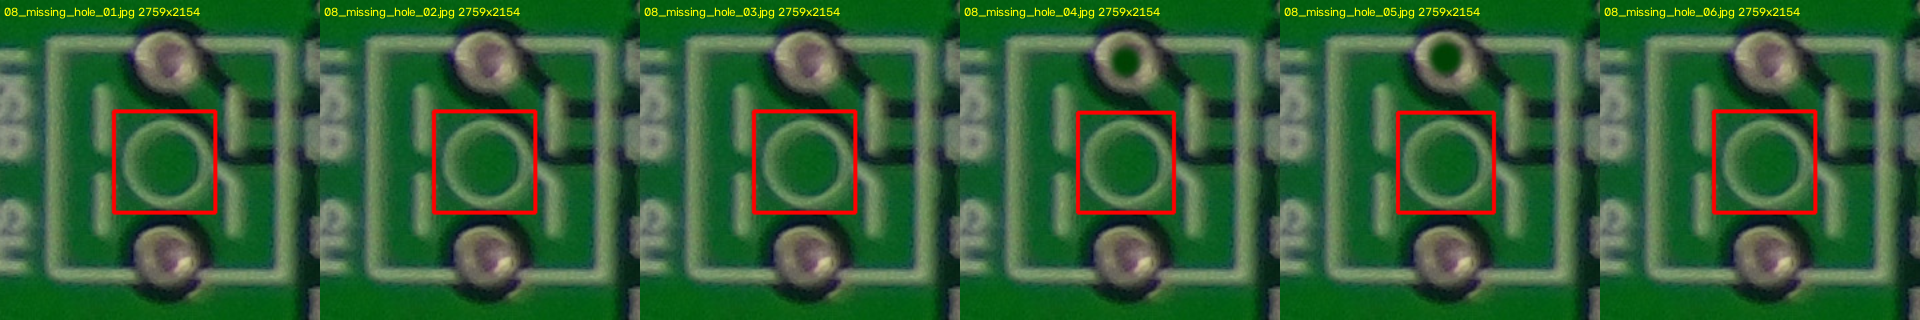
\includegraphics[width=\linewidth]{../../results/hotspot2_08_180_1080.png}
\subcaption{Bo 08, lớp dự đoán Missing Hole, tâm khoảng $(180, 1080)$: box thừa ở 60 ảnh, độ tin cậy trung bình $0.59$.}
\end{subfigure}
\vspace{4pt}
\begin{subfigure}[t]{\linewidth}
\centering
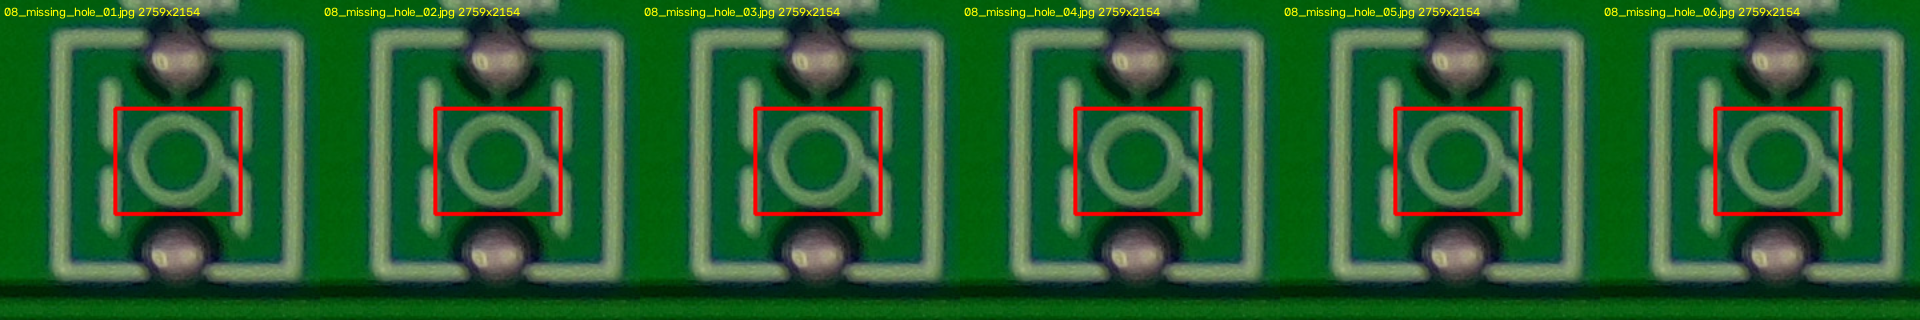
\includegraphics[width=\linewidth]{../../results/hotspot2_08_1740_510.png}
\subcaption{Bo 08, lớp dự đoán Missing Hole, tâm khoảng $(1740, 510)$: box thừa ở 59 ảnh, độ tin cậy trung bình $0.34$.}
\end{subfigure}
\vspace{4pt}
\begin{subfigure}[t]{\linewidth}
\centering
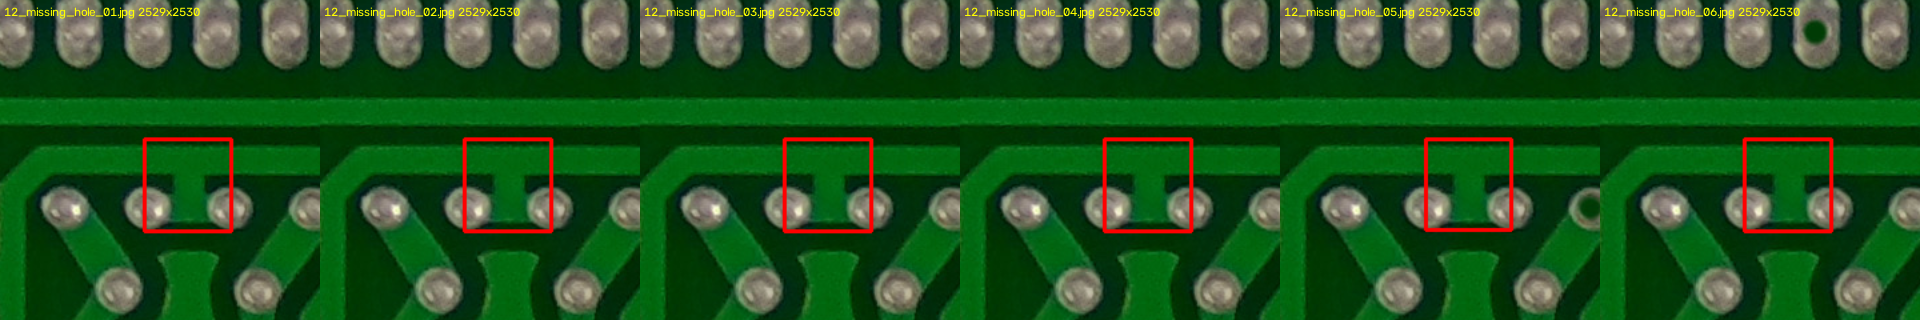
\includegraphics[width=\linewidth]{../../results/hotspot2_12_1170_1140.png}
\subcaption{Bo 12, lớp dự đoán Short, tâm khoảng $(1170, 1140)$: box thừa ở 60 ảnh, độ tin cậy trung bình $0.63$.}
\end{subfigure}
\vspace{4pt}
\begin{subfigure}[t]{\linewidth}
\centering
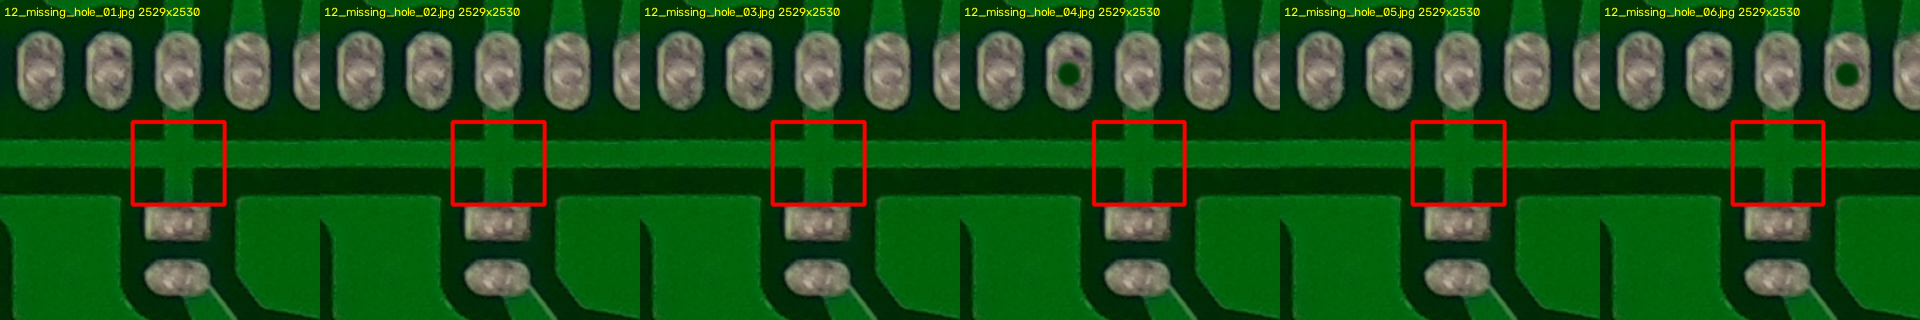
\includegraphics[width=\linewidth]{../../results/hotspot2_12_1560_1110.png}
\subcaption{Bo 12, lớp dự đoán Short, tâm khoảng $(1560, 1110)$: box thừa ở 60 ảnh, độ tin cậy trung bình $0.39$.}
\end{subfigure}
\vspace{4pt}
\begin{subfigure}[t]{\linewidth}
\centering
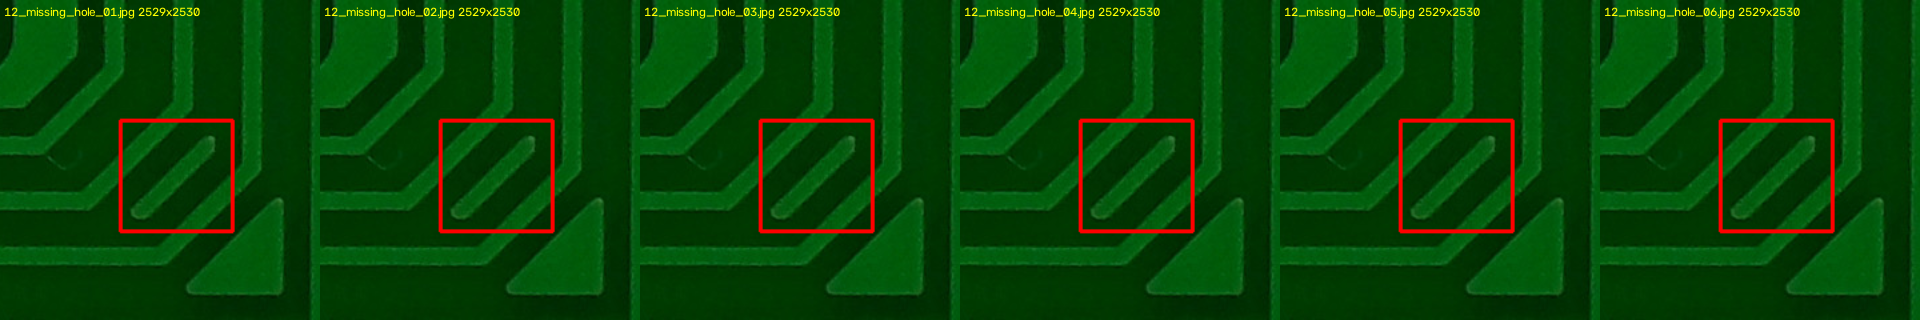
\includegraphics[width=\linewidth]{../../results/hotspot2_12_1710_1560.png}
\subcaption{Bo 12, lớp dự đoán Spurious Copper, tâm khoảng $(1710, 1560)$: box thừa ở 51 ảnh, độ tin cậy trung bình $0.32$.}
\end{subfigure}
\caption{Năm vị trí box thừa lặp lại trên test (conf $0.25$). Mỗi dải gồm 6 trong số các ảnh của cùng một bo, cắt quanh một vị trí; khung đỏ là box thừa, luôn nằm đúng một chỗ trên các ảnh khác nhau. Số ảnh và độ tin cậy lấy từ \texttt{reports/bang\_so\_lieu.md}, mục 5.}
\label{fig:hotspot}
\end{figure}

\begin{luuy}[title={Nhận định}]
Bộ phát hiện một giai đoạn chỉ thấy một ảnh, không có ảnh mẫu để đối chiếu, nên trên bo chưa từng thấy khi huấn luyện nó nhầm chi tiết thiết kế cố định với lỗi. Đây là lý do dùng ảnh bo mẫu để kiểm chứng box ở Chương 7.
\end{luuy}

\muc{6.5. Chọn ngưỡng độ tin cậy theo lớp}

\begin{itemize}
  \item \textbf{Cách chọn} (\texttt{tools/select\_thresholds.py}, chỉ trên val): thử conf $\in\{0.25, 0.4, 0.5, 0.6\}$. Với mỗi lớp, chỉ xét các ngưỡng có recall $\ge 0.90$ (nếu không có ngưỡng nào thì lấy ngưỡng có recall cao nhất), rồi chọn ngưỡng có F1 cao nhất; hòa thì lấy conf thấp hơn.
  \item \textbf{Ngưỡng chung:} $0.25$ (macro-F1 cao nhất trên val). Đây cũng là conf mặc định của demo.
  \item \textbf{Kết quả:} mọi lớp dùng $0.25$, riêng \textbf{Short} dùng $0.5$.
\end{itemize}

\needspace{12\baselineskip}
\begin{table}[H]
\centering
\small
\caption{$P / R / F1$ trên val theo ngưỡng conf (\texttt{configs/thresholds.json})}\label{tab:nguong}
\begin{tabular}{l|ccc|ccc|c}
\toprule
 & \multicolumn{3}{c|}{conf $0.25$} & \multicolumn{3}{c|}{conf $0.5$} & \textbf{Chọn} \\
\textbf{Lớp} & $P$ & $R$ & $F1$ & $P$ & $R$ & $F1$ & \\ \midrule
Missing Hole & 1.000 & 1.00 & 1.000 & 1.000 & 1.00 & 1.000 & 0.25 \\
Mouse Bite & 0.990 & 0.96 & 0.975 & 1.000 & 0.93 & 0.964 & 0.25 \\
Open Circuit & 0.990 & 1.00 & 0.995 & 0.990 & 1.00 & 0.995 & 0.25 \\
Short & 0.901 & 0.99 & 0.943 & 0.943 & 0.98 & 0.961 & \textbf{0.5} \\
Spur & 0.949 & 0.93 & 0.939 & 0.988 & 0.81 & 0.890 & 0.25 \\
Spurious Copper & 0.952 & 0.98 & 0.966 & 0.969 & 0.931 & 0.949 & 0.25 \\ \bottomrule
\end{tabular}
\end{table}
\begin{itemize}
  \item \textbf{Short} là lớp duy nhất được lợi khi nâng ngưỡng: precision tăng từ $0.901$ lên $0.943$, recall chỉ giảm $0.99 \to 0.98$. Các lớp khác nâng ngưỡng làm recall giảm nhiều hơn mức precision tăng (rõ nhất ở Spur: $0.93 \to 0.81$).
\end{itemize}

%=====================================================================
\chuong{CHƯƠNG 7: KẾT HỢP YOLO + XOR}
\sochuong{7}
%=====================================================================

\muc{7.1. Ý tưởng và quy tắc lọc}

Chi tiết thiết kế cố định của bo giống hệt ảnh bo mẫu, nên XOR không thấy khác biệt ở đó. Lỗi thật làm ảnh khác ảnh mẫu, nên có pixel khác biệt trong box.

\begin{enumerate}
  \item Đưa box YOLO (khung ảnh lỗi) sang khung ảnh mẫu bằng $H$, lấy hộp bao.
  \item Tính mặt nạ khác biệt: XOR, giữ vùng hợp lệ, median $5\times5$, đóng $27\times27$, mở $3\times3$.
  \item Đếm số pixel khác biệt $n(b)$ và tỉ lệ vùng hợp lệ $v(b)$ trong box mở rộng thêm $\mathit{pad}=8$ px.
\end{enumerate}

Ký hiệu cụ thể: gọi $b_t$ là hộp bao của bốn góc của $b$ sau khi ánh xạ bằng $H$, và $b_t^{+}$ là $b_t$ mở rộng $\mathit{pad}$ pixel mỗi phía. Với mặt nạ khác biệt $M\in\{0,1\}$ và mặt nạ vùng hợp lệ $V\in\{0,1\}$ (cùng khung ảnh mẫu):
\begin{equation}\label{eq:nb}
n(b)=\sum_{(x,y)\in b_t^{+}} M(x,y),
\qquad
v(b)=\frac{1}{\lvert b_t^{+}\rvert}\sum_{(x,y)\in b_t^{+}} V(x,y).
\end{equation}

\begin{dly}[title={Quy tắc giữ box}]
Giữ box $b$ khi
\[ n(b) \ge \mathit{min\_px} \quad\text{hoặc}\quad v(b) < \mathit{min\_valid} \qquad (\mathit{min\_valid}=0.5). \]
Box không xác minh được (nằm sát viền warp) thì \textbf{giữ}, để không mất box đúng vì căn chỉnh hay viền. Ảnh căn chỉnh thất bại thì giữ nguyên mọi box YOLO.
\end{dly}

\hinhref{trucquan} giải thích vì sao phép kiểm này loại được box thừa mà không động đến box đúng, và \hinhref{locflow} là lưu đồ của bộ lọc; \thuattoanref{loc} là mã giả.

\begin{figure}[H]
\centering
\begin{tikzpicture}[x=1cm,y=1cm,scale=1.1,transform shape]
% (a) ảnh lỗi + hai box YOLO
\begin{scope}[shift={(0,0)}]\pcbmau{1}
  \draw[cyan!75!white,very thick,dashed] (0.05,0.2) rectangle (0.65,0.8);
  \draw[cyan!75!white,very thick] (1.3,0.62) rectangle (1.9,1.08);
  \node[font=\scriptsize,cyan!85!white,fill=nenmach,inner sep=1pt] at (0.9,0.0) {$b_1$};
  \node[font=\scriptsize,cyan!85!white,fill=nenmach,inner sep=1pt] at (2.15,0.85) {$b_2$};
\end{scope}
% (b) bản đồ khác biệt XOR sau xử lý
\begin{scope}[shift={(4.4,0)}]\pcbxor{0}
  \draw[cyan!75!white,very thick,dashed] (0.05,0.2) rectangle (0.65,0.8);
  \draw[cyan!75!white,very thick] (1.3,0.62) rectangle (1.9,1.08);
\end{scope}
\draw[mui] (3.35,1.1)--(4.25,1.1) node[midway,above,font=\tiny\itshape]{$H$, XOR};
% (c) quyết định
\node[khoi do,text width=46mm,font=\scriptsize,align=left,anchor=west] (k1) at (8.2,1.95) {\textbf{$b_1$:} không có pixel khác biệt\\$n(b_1)<\mathit{min\_px}$ $\Rightarrow$ \textbf{loại} (chi tiết cố định của bo)};
\node[khoi ra,text width=46mm,font=\scriptsize,align=left,anchor=west] (k2) at (8.2,0.25) {\textbf{$b_2$:} có vùng khác biệt\\$n(b_2)\ge\mathit{min\_px}$ $\Rightarrow$ \textbf{giữ} (lỗi thật)};
\node[font=\scriptsize,align=center] at (1.6,-0.65) {(a) ảnh lỗi và hai box YOLO};
\node[font=\scriptsize,align=center] at (6.0,-0.65) {(b) bản đồ khác biệt $M$};
\node[font=\scriptsize,align=center] at (10.55,-0.65) {(c) quyết định của bộ lọc};
\end{tikzpicture}
\caption{Ý tưởng của bộ lọc (sơ đồ minh hoạ, không phải ảnh thật): chi tiết thiết kế cố định giống hệt ảnh bo mẫu nên XOR trống, còn lỗi thật để lại pixel khác biệt.}
\label{fig:trucquan}
\end{figure}

\begin{figure}[H]
\centering
\begin{tikzpicture}[x=1cm,y=1cm]
\tikzset{nhan/.append style={font=\scriptsize\itshape}}\node[khoi vao,text width=36mm] (st) at (0,0) {Box YOLO $b$,\\ảnh mẫu, $H$};
\node[khoi,text width=48mm] (s1) at (0,-1.75) {Ánh xạ $b$ sang khung ảnh mẫu bằng $H$,\\lấy hộp bao, mở rộng $\mathit{pad}=8$ px};
\node[khoi,text width=48mm] (s2) at (0,-3.5) {Tính $n(b)$ và $v(b)$ trên\\mặt nạ khác biệt $M$ và vùng hợp lệ $V$};
\node[quyet,text width=33mm] (q1) at (0,-5.7) {$v(b)<\mathit{min\_valid}$\\($0.5$)?};
\node[quyet,text width=33mm] (q2) at (0,-8.8) {$n(b)\ge\mathit{min\_px}$\\($10$)?};
\node[khoi ra,text width=30mm] (keep) at (6.2,-7.3) {\textbf{Giữ box}};
\node[khoi do,text width=30mm] (drop) at (0,-11.0) {\textbf{Loại box}\\(không có bằng chứng thay đổi)};
\foreach \i/\j in {st/s1,s1/s2,s2/q1}{\draw[mui] (\i)--(\j);}
\draw[mui] (q1)--node[left,nhan]{không}(q2);
\draw[mui] (q2)--node[left,nhan]{không}(drop);
\draw[mui] (q1.east)-|node[pos=0.25,above,nhan]{có: không xác minh được}(keep.north);
\draw[mui] (q2.east)-|node[pos=0.25,above,nhan]{có: có bằng chứng}(keep.south);
\node[khoi,text width=40mm,font=\tiny,draw=gray!60,fill=gray!8,anchor=west] at (4.1,-1.0) {Căn chỉnh thất bại: giữ nguyên mọi box YOLO};
\end{tikzpicture}
\caption{Lưu đồ bộ lọc YOLO + XOR cho một box.}
\label{fig:locflow}
\end{figure}

\begin{algorithm}[H]
\caption{Lọc box YOLO bằng bản đồ khác biệt XOR}\label{alg:loc}
\KwIn{ảnh lỗi $I_d$; ảnh bo mẫu $I_t$; tập box YOLO $\mathcal{B}$; $\mathit{min\_px}{=}10$, $\mathit{pad}{=}8$, $\mathit{min\_valid}{=}0.5$}
\KwOut{tập box đã lọc $\mathcal{B}'$}
$(H,\,I_w) \leftarrow \text{\thuattoanref{sift}}(I_d,\,I_t)$\;
\If{căn chỉnh thất bại}{
  \KwRet{$\mathcal{B}$} \tcp*{giữ nguyên mọi box}
}
$(M,\,V) \leftarrow$ XOR, median $5{\times}5$, đóng $27{\times}27$, mở $3{\times}3$; và vùng hợp lệ\;
$\mathcal{B}' \leftarrow \emptyset$\;
\ForEach{box $b \in \mathcal{B}$}{
  $b_t^{+} \leftarrow \mathrm{expand}\bigl(\mathrm{bbox}(\pi(H\,\mathrm{góc}(b))),\ \mathit{pad}\bigr)$\;
  tính $n(b),\,v(b)$ theo công thức (\ref{eq:nb})\;
  \If{$n(b) \ge \mathit{min\_px}$ \textbf{hoặc} $v(b) < \mathit{min\_valid}$}{
    $\mathcal{B}' \leftarrow \mathcal{B}' \cup \{b\}$ \tcp*{có bằng chứng, hoặc không xác minh được}
  }
}
\KwRet{$\mathcal{B}'$}
\end{algorithm}

\muc{7.2. Chọn tham số trên val}

Thử $\mathit{min\_px}\in\{0,10,25,50,100,200,400,800\}$ ($0$ nghĩa là không lọc). Nhận $\mathit{min\_px}$ nếu recall val giảm không quá $0.01$ so với YOLO thuần; trong các giá trị nhận được, chọn F1 cao nhất, hòa thì lấy giá trị nhỏ.

\needspace{12\baselineskip}
\begin{table}[H]
\centering
\small
\caption{Quét \texttt{min\_px} trên val (\texttt{results/fusion\_val\_sweep.csv})}\label{tab:quetminpx}
\begin{tabular}{r|rrr|ccc}
\toprule
\textbf{min\_px} & \textbf{TP} & \textbf{FP} & \textbf{FN} & $P$ & $R$ & $F1$ \\ \midrule
0 (YOLO thuần) & 588 & 18 & 15 & 0.9703 & 0.9751 & 0.9727 \\
\textbf{10} & 588 & 17 & 15 & 0.9719 & 0.9751 & 0.9735 \\
25 & 588 & 17 & 15 & 0.9719 & 0.9751 & 0.9735 \\
50 & 588 & 17 & 15 & 0.9719 & 0.9751 & 0.9735 \\
100 & 588 & 17 & 15 & 0.9719 & 0.9751 & 0.9735 \\
200 & 584 & 17 & 19 & 0.9717 & 0.9685 & 0.9701 \\
400 & 555 & 15 & 48 & 0.9737 & 0.9204 & 0.9463 \\
800 & 293 & 12 & 310 & 0.9607 & 0.4859 & 0.6454 \\ \bottomrule
\end{tabular}
\end{table}
\begin{itemize}
  \item Chọn $\mathit{min\_px}=10$ (lưu ở \texttt{configs/fusion.json}, cùng $\mathit{pad}=8$, $\mathit{min\_valid}=0.5$).
  \item Trên val chỉ có 18 box thừa nên F1 gần như không đổi ($0.9727 \to 0.9735$). Tác dụng lộ rõ ở test.
\end{itemize}

\hinhref{sweep} vẽ lại \bangref{quetminpx}: precision gần như không đổi, còn recall giữ ổn định đến $\mathit{min\_px}=100$ rồi giảm dần và tụt nhanh ở $400$ và $800$.

\begin{figure}[H]
\centering
\begin{tikzpicture}
\begin{axis}[width=0.9\linewidth,height=6.2cm,
  symbolic x coords={0,10,25,50,100,200,400,800},xtick=data,
  xlabel={$\mathit{min\_px}$ (0 = YOLO thuần)},ylabel={Chỉ số trên val},ymin=0.4,ymax=1.02,
  tick label style={font=\scriptsize},label style={font=\footnotesize},
  grid=both,grid style={gray!20},axis line style={gray!60},
  legend style={font=\scriptsize,at={(0.02,0.04)},anchor=south west,draw=gray!40,fill=white}]
\addplot[mark=*,thick,blue!60!black] coordinates {(0,0.9703)(10,0.9719)(25,0.9719)(50,0.9719)(100,0.9719)(200,0.9717)(400,0.9737)(800,0.9607)};
\addplot[mark=square*,thick,orange!85!black] coordinates {(0,0.9751)(10,0.9751)(25,0.9751)(50,0.9751)(100,0.9751)(200,0.9685)(400,0.9204)(800,0.4859)};
\addplot[mark=triangle*,thick,green!50!black] coordinates {(0,0.9727)(10,0.9735)(25,0.9735)(50,0.9735)(100,0.9735)(200,0.9701)(400,0.9463)(800,0.6454)};
\addplot[red!70!black,dashed,no marks] coordinates {(0,0.9651)(800,0.9651)};
\legend{$P$,$R$,$F1$,{ngưỡng recall $0.9751-0.01$}}
\node[pin={[pin distance=1.1cm,font=\scriptsize,pin edge={thick,black!70}]-40:{được chọn: 10}}] at (axis cs:10,0.9735) {};
\end{axis}
\end{tikzpicture}
\caption{Quét $\mathit{min\_px}$ trên val. Từ $400$ trở lên recall tụt dưới ngưỡng cho phép (đường đỏ nét đứt), nên chọn $\mathit{min\_px}=10$ (F1 cao nhất trong các giá trị được nhận).}
\label{fig:sweep}
\end{figure}

\needspace{17\baselineskip}
\muc{7.3. Kết quả trên test (chạy một lần)}

Cách tính: ngưỡng conf theo lớp (Mục 6.5), khớp \textbf{cùng lớp}, IoU $\ge 0.5$, $P$ và $R$ \textbf{gộp} trên mọi box (không phải trung bình theo lớp của Ultralytics).

\begin{table}[H]
\centering
\small
\caption{Tác dụng của bộ lọc XOR trên test theo lớp (conf theo lớp, IoU $0.5$, khớp cùng lớp)}\label{tab:loctest}
\begin{tabular}{l|rr|rr|cc|cc}
\toprule
 & & & \multicolumn{2}{c|}{\textbf{FP}} & \multicolumn{2}{c|}{$P$} & \multicolumn{2}{c}{$F1$} \\
\textbf{Lớp} & \textbf{TP} & \textbf{FN} & YOLO & +XOR & YOLO & +XOR & YOLO & +XOR \\ \midrule
Missing Hole & 99 & 2 & 238 & 0 & 0.2938 & 1.0000 & 0.4521 & 0.9900 \\
Mouse Bite & 96 & 4 & 8 & 8 & 0.9231 & 0.9231 & 0.9412 & 0.9412 \\
Open Circuit & 98 & 2 & 1 & 1 & 0.9899 & 0.9899 & 0.9849 & 0.9849 \\
Short & 99 & 0 & 61 & 2 & 0.6188 & 0.9802 & 0.7645 & 0.9900 \\
Spur & 83 & 18 & 1 & 1 & 0.9881 & 0.9881 & 0.8973 & 0.8973 \\
Spurious Copper & 98 & 2 & 59 & 8 & 0.6242 & 0.9245 & 0.7626 & 0.9515 \\ \midrule
\textbf{Tổng} & \textbf{573} & \textbf{28} & \textbf{368} & \textbf{20} & \textbf{0.6089} & \textbf{0.9663} & \textbf{0.7432} & \textbf{0.9598} \\ \bottomrule
\end{tabular}
\end{table}

\begin{itemize}
  \item Bộ lọc loại \textbf{348/368} box thừa và \textbf{không mất box đúng nào} ($TP=573$ giữ nguyên, $R=0.9534$ không đổi).
  \item $P$ tăng $0.6089 \to 0.9663$; $F1$ tăng $0.7432 \to 0.9598$.
  \item Cải thiện lớn nhất ở Missing Hole (FP $238 \to 0$), Short ($61 \to 2$) và Spurious Copper ($59 \to 8$). Đây cũng là các lớp có nhiều box thừa ở vị trí cố định (Mục 6.4).
  \item Mouse Bite, Open Circuit, Spur không đổi vì box thừa của các lớp này không nằm ở chi tiết cố định.
\end{itemize}

\hinhref{fptest} (số liệu ở \bangref{loctest}) cho thấy bộ lọc gần như xoá hết box thừa ở ba lớp có chi tiết cố định (Missing Hole, Short, Spurious Copper) mà không đổi recall.

\begin{figure}[H]
\centering
\begin{subfigure}[t]{0.57\linewidth}
\centering
\begin{tikzpicture}
\begin{axis}[bieudo,width=\linewidth,height=5.6cm,ymax=330,bar width=7pt,
  symbolic x coords={MH,MB,OC,SH,SP,SC},xtick=data,ylabel={Số box thừa (FP)},
  /pgf/number format/precision=0]
\addplot[fill=gray!55,draw=gray!70!black] coordinates {(MH,238)(MB,8)(OC,1)(SH,61)(SP,1)(SC,59)};
\addplot[fill=blue!45!black!70,draw=chinh] coordinates {(MH,0)(MB,8)(OC,1)(SH,2)(SP,1)(SC,8)};
\legend{YOLO,YOLO + XOR}
\end{axis}
\end{tikzpicture}
\subcaption{Box thừa theo lớp}
\end{subfigure}\hfill
\begin{subfigure}[t]{0.41\linewidth}
\centering
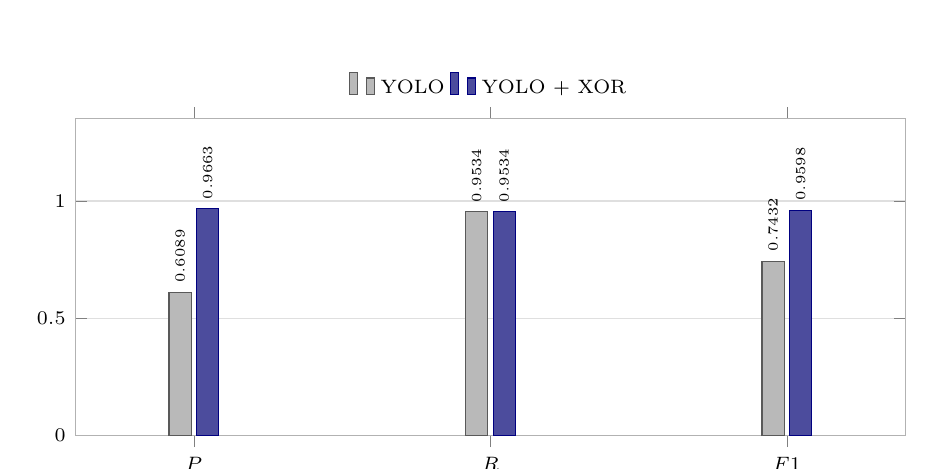
\begin{tikzpicture}
\begin{axis}[bieudo,width=\linewidth,height=5.6cm,ymax=1.35,bar width=8pt,
  symbolic x coords={P,R,F1},xtick=data,xticklabels={$P$,$R$,$F1$},
  /pgf/number format/precision=4]
\addplot[fill=gray!55,draw=gray!70!black] coordinates {(P,0.6089)(R,0.9534)(F1,0.7432)};
\addplot[fill=blue!45!black!70,draw=chinh] coordinates {(P,0.9663)(R,0.9534)(F1,0.9598)};
\legend{YOLO,YOLO + XOR}
\end{axis}
\end{tikzpicture}
\subcaption{Chỉ số tổng}
\end{subfigure}
\caption{Tác dụng của bộ lọc XOR trên test (conf theo lớp, IoU $0.5$, khớp cùng lớp). Box thừa giảm từ $368$ xuống $20$; recall giữ nguyên.}
\label{fig:fptest}
\end{figure}

\muc{7.4. So sánh ba hướng trên test}

\begin{table}[H]
\centering
\small
\caption{So sánh ba hướng trên test}\label{tab:bahuong}
\begin{tabular}{p{3.6cm}|p{5.4cm}|ccc}
\toprule
\textbf{Hướng} & \textbf{Cách tính} & $P$ & $R$ & \textbf{F1 / mAP50} \\ \midrule
YOLOv8s (Ultralytics) & $P$, $R$, mAP do Ultralytics tính & 0.8543 & 0.9336 & mAP50 0.9720 \\
YOLOv8s (conf theo lớp) & gộp, IoU $0.5$, cùng lớp & 0.6089 & 0.9534 & F1 0.7432 \\
SIFT + XOR (\texttt{new}) & chỉ phát hiện, không xét lớp, IoU $0.5$ & 0.6555 & 0.6206 & F1 0.6376 \\
YOLOv8s + lọc XOR & gộp, IoU $0.5$, cùng lớp & 0.9663 & 0.9534 & F1 0.9598 \\ \bottomrule
\end{tabular}
\end{table}
\begin{itemize}
  \item Với đường XOR, phân loại đúng $0.9169$ ($342/373$) trên các box tìm đúng (Mục 5.4).
  \item Chỉ so sánh trực tiếp hai dòng \emph{cùng cách tính}: YOLOv8s (conf theo lớp) và YOLOv8s + lọc XOR.
\end{itemize}

\begin{luuy}[title={Về hai cách đếm box thừa}]
Số box thừa ở Mục 6.3 (Missing Hole $119$, Short $123$) dùng conf $0.25$ chung và ghép không xét lớp. Số ở Mục 7.3 (Missing Hole $238$, Short $61$) dùng conf theo lớp và ghép cùng lớp. Hai bảng dùng cách ghép và ngưỡng khác nhau, nên chỉ so sánh trong nội bộ từng bảng.
\end{luuy}

\muc{7.5. Hạn chế của bộ lọc}

\begin{itemize}
  \item \textbf{Cần ảnh bo mẫu} của đúng bo đang kiểm tra và căn chỉnh SIFT thành công.
  \item \textbf{Chỉ loại box thừa}, không cứu được box bị bỏ sót. Recall giữ nguyên $0.9534$; Spur vẫn thấp nhất ($0.8218$, 18 box bỏ sót).
  \item Kết quả test dựa trên 2 bo (08, 12).
\end{itemize}

%=====================================================================
\chuong{CHƯƠNG 8: DEMO VÀ KIỂM THỬ}
\sochuong{8}
%=====================================================================

\muc{8.1. Ứng dụng Gradio}

Chạy bằng \texttt{python demo/app.py} (mặc định \texttt{http://127.0.0.1:7860}). Trọng số đặt trong \texttt{models/}: \texttt{best.pt} (bộ phát hiện, bắt buộc) và \texttt{best\_cls.pt} (bộ phân loại, cần cho tab 2, 3, 4), hoặc nạp từ Hugging Face qua biến \texttt{HF\_MODEL\_REPO}.

\begin{table}[H]
\centering
\small
\caption{Các tab của ứng dụng demo}\label{tab:demotab}
\begin{tabular}{l|>{\raggedright\arraybackslash}p{4.2cm}|>{\raggedright\arraybackslash}p{6.4cm}}
\toprule
\textbf{Tab} & \textbf{Đầu vào} & \textbf{Phương pháp} \\ \midrule
1. Phát hiện nhanh & một ảnh & YOLOv8s (\texttt{imgsz} 1024) \\
2. Đối chiếu ảnh mẫu & ảnh lỗi + ảnh bo mẫu & SIFT, XOR, bộ phân loại ảnh cắt (hướng của bài báo) \\
3. Đối chiếu hai hướng & ảnh lỗi + ảnh bo mẫu & cả hai hướng trên, ghép box ở IoU $\ge 0.1$ (xanh lá: cả hai, xanh dương: chỉ YOLO, cam: chỉ XOR) \\
4. YOLO + lọc XOR & ảnh lỗi + ảnh bo mẫu & bộ lọc ở Chương 7 \\
Thông tin mô hình & -- & mã băm trọng số, phiên bản, kết quả đo trên test, giới hạn đã biết \\ \bottomrule
\end{tabular}
\end{table}

Mỗi phân tích trả về: ảnh đã vẽ box, tóm tắt, bảng từng vùng, ảnh cắt cận cảnh, và file CSV, JSON để tải (JSON ghi tham số, thời gian, thiết bị, mã băm trọng số).

\begin{luuy}
Quy tắc đối chiếu hai hướng (tab 3) mang tính minh họa, \textbf{chưa được đánh giá} như một phương pháp riêng. Phương pháp được đánh giá là bộ lọc ở tab 4 (Chương 7). Demo là công cụ nghiên cứu và giảng dạy, không phải hệ thống kiểm tra sản xuất.
\end{luuy}

\hinhref{demoarch} cho thấy các thành phần của ứng dụng và vị trí của các cơ chế an toàn ở Mục 8.2.

\begin{figure}[H]
\centering
\begin{tikzpicture}[x=1cm,y=1cm,scale=0.9,transform shape]
\node[khoi vao,text width=38mm] (u) at (4.5,0) {\textbf{Người dùng} (trình duyệt)\\ảnh lỗi, ảnh bo mẫu tuỳ tab};
\node[khoi,text width=38mm] (in) at (4.5,-1.9) {\textbf{Kiểm tra đầu vào}\\loại file, $\le30$ MB, giải mã,\\cạnh nhỏ nhất 256 px};
\node[khoi,text width=38mm] (tab) at (4.5,-3.8) {\textbf{Gradio} (\texttt{demo/app.py})\\4 tab phân tích và\\thông tin mô hình};
\node[khoi moi,text width=21mm] (m1) at (0.9,-6.0) {\textbf{YOLOv8s}\\\texttt{best.pt}};
\node[khoi moi,text width=21mm] (m2) at (4.5,-6.0) {\textbf{SIFT + XOR}\\(OpenCV)};
\node[khoi moi,text width=21mm] (m3) at (8.1,-6.0) {\textbf{YOLOv8n-cls}\\\texttt{best\_cls.pt}};
\node[khoi ra,text width=60mm] (out) at (4.5,-8.1) {Ảnh vẽ box, tóm tắt, bảng từng vùng, ảnh cắt cận cảnh,\\file CSV và JSON (tham số, thời gian, thiết bị, mã băm trọng số)};
\draw[mui] (u)--(in); \draw[mui] (in)--(tab);
\draw[mui] (tab.south)--++(0,-0.35)-|(m1.north);
\draw[mui] (tab.south)--(m2.north);
\draw[mui] (tab.south)--++(0,-0.35)-|(m3.north);
\draw[mui] (m1.south)|-++(0,-0.4)-|(out.north west);
\draw[mui] (m2.south)--(out.north);
\draw[mui] (m3.south)|-++(0,-0.4)-|(out.north east);
% trọng số
\node[khoi vao,text width=24mm] (w) at (-3.0,-6.0) {Trọng số\\\texttt{models/} hoặc\\\texttt{HF\_MODEL\_REPO}};
\draw[mui net] (w)--(m1);
% cơ chế an toàn
\node[khoi do,text width=34mm,font=\scriptsize] (s1) at (11.4,-1.9) {Từ chối trọng số có tên lớp bị hoán vị};
\node[khoi do,text width=34mm,font=\scriptsize] (s2) at (11.4,-3.55) {Tự kiểm bộ phân loại bằng 12 ảnh cắt (\texttt{canary}) khi khởi động};
\node[khoi do,text width=34mm,font=\scriptsize] (s3) at (11.4,-5.2) {Hết bộ nhớ GPU: chuyển sang CPU một lần};
\node[khoi do,text width=34mm,font=\scriptsize] (s4) at (11.4,-6.85) {Căn chỉnh thất bại: trả thông báo thay vì lỗi hệ thống};
\node[tieude,font=\scriptsize\bfseries,text=red!65!black] at (9.5,-0.75) {Cơ chế an toàn};
\begin{scope}[on background layer]
 \node[fit=(s1)(s2)(s3)(s4),fill=red!3,draw=red!25,dashed,rounded corners=4pt,inner sep=6pt] {};
\end{scope}
\end{tikzpicture}
\caption{Kiến trúc ứng dụng demo và các cơ chế an toàn (khung đỏ nét đứt).}
\label{fig:demoarch}
\end{figure}

\muc{8.2. Cơ chế an toàn}

\begin{itemize}
  \item \textbf{Kiểm tra tên lớp:} từ chối trọng số còn mang tên lớp bị hoán vị (Mục 2.5) và in ra lệnh sửa.
  \item \textbf{Tự kiểm bộ phân loại:} khi khởi động, phân loại 12 ảnh cắt tham chiếu trong \texttt{demo/assets/\allowbreak canary/}; hiện biểu ngữ đỏ nếu đa số bị sai (bắt được trường hợp \texttt{best\_cls.pt} chưa sửa tên lớp mà kiểm tra tên lớp không thấy).
  \item \textbf{Kiểm tra đầu vào:} loại file, dung lượng (mặc định tối đa 30 MB), khả năng giải mã, cạnh nhỏ nhất 256 px; xử lý được tên file không phải ASCII.
  \item \textbf{Hết bộ nhớ GPU:} tự chuyển sang CPU một lần và thông báo trong kết quả.
  \item \textbf{Căn chỉnh thất bại} (sai ảnh mẫu, không đủ đặc trưng chung, homography vô lý): trả thông báo thay vì lỗi hệ thống.
  \item Mở trên địa chỉ không phải localhost mà không có \texttt{--auth} thì ghi cảnh báo vào log.
\end{itemize}

\muc{8.3. Kiểm thử, CI và đóng gói}

\begin{itemize}
  \item \textbf{Kiểm thử:} \texttt{pytest} với 32 hàm kiểm thử trong \texttt{tests/}, dùng mô hình giả nên không cần trọng số hay GPU. Bao phủ kiểm tra đầu vào, kiểm tra tên lớp, sắp xếp và xuất file, chuyển sang CPU khi hết bộ nhớ, đường ảnh mẫu trên bo tổng hợp, đối chiếu hai hướng, tự kiểm bộ phân loại và hàm lọc ở Chương 7.
  \item \textbf{CI:} GitHub Actions chạy \texttt{pytest} trên Python 3.12 mỗi lần \texttt{push} lên \texttt{main} và mỗi \texttt{pull request}.
  \item \textbf{Docker (CPU):} ảnh dựa trên \texttt{python:3.12-slim}, cài PyTorch bản CPU, \texttt{ultralytics==8.4.194} và Gradio. Trọng số \textbf{không} nằm trong ảnh, mà gắn vào \texttt{/app/models} hoặc nạp qua \texttt{HF\_MODEL\_REPO}. Chạy với người dùng không phải root, có \texttt{HEALTHCHECK}, cổng 7860.
  \item \textbf{Cấu hình:} mọi giá trị đặt được bằng biến môi trường \texttt{PCB\_*} (thiết bị, conf, host, cổng, tài khoản, giới hạn tải lên) hoặc tham số dòng lệnh.
\end{itemize}

\muc{8.4. Ảnh chụp giao diện demo}

% TODO: chụp màn hình từng tab và chèn hình (README của demo yêu cầu thêm ảnh mẫu vào demo/examples/)
\trong[4cm]

\muc{8.5. Đưa trọng số và demo lên Hugging Face}

% TODO: ghi liên kết kho mô hình / Space sau khi đã đăng lên (README mới có lệnh hf upload, chưa có tên kho thật)
\trong[3cm]

%=====================================================================
\chuong{CHƯƠNG 9: TIẾN ĐỘ THỰC HIỆN, SẢN PHẨM VÀ KHẢ NĂNG ỨNG DỤNG}
\sochuong{9}
%=====================================================================

\muc{9.1. Tiến độ thực hiện}

\begin{table}[H]
\centering
\small
\caption{Tiến độ thực hiện}\label{tab:tiendo}
\begin{tabular}{c|>{\raggedright\arraybackslash}p{9.2cm}|>{\raggedright\arraybackslash}c|>{\raggedright\arraybackslash}c}
\toprule
\textbf{TT} & \textbf{Công việc} & \textbf{Chương} & \textbf{Trạng thái} \\ \midrule
1 & Tìm hiểu bài toán, bộ dữ liệu và tài liệu liên quan & 1 & Hoàn thành \\
2 & Chuyển nhãn, chia theo bo, kiểm toán rò rỉ & 2 & Hoàn thành \\
3 & Huấn luyện và so sánh các mô hình YOLOv8 & 3, 5 & Hoàn thành \\
4 & Cài đặt đường SIFT + XOR và bộ phân loại ảnh cắt & 4, 5 & Hoàn thành \\
5 & Phân tích lỗi, chọn ngưỡng theo lớp & 6 & Hoàn thành \\
6 & Đề xuất và đánh giá bộ lọc YOLO + XOR & 7 & Hoàn thành \\
7 & Xây dựng demo, kiểm thử, CI, Docker & 8 & Hoàn thành \\
8 & Phát hiện và sửa lỗi hoán vị tên lớp, đánh giá lại & 2.5 & Hoàn thành \\
9 & Chụp giao diện demo, đăng trọng số và demo lên Hugging Face & 8.4, 8.5 & Chưa thực hiện \\
10 & Hoàn thiện báo cáo & -- & Đang thực hiện \\ \bottomrule
\end{tabular}
\end{table}

\textbf{Các mốc có ghi nhận:} ngày 06/10/2026 chạy huấn luyện đầu tiên (\texttt{pcb\_v8s}); ngày 03/11/2026 phát hiện và sửa lỗi hoán vị tên lớp; tháng 11/2026 hoàn thiện báo cáo.

\muc{9.2. Sản phẩm đề tài}

\begin{table}[H]
\centering
\small
\caption{Sản phẩm của đề tài}\label{tab:sanpham}
\begin{tabular}{>{\raggedright\arraybackslash}p{3.6cm}|>{\raggedright\arraybackslash}p{6.4cm}|>{\raggedright\arraybackslash}p{4.4cm}}
\toprule
\textbf{Sản phẩm} & \textbf{Mô tả} & \textbf{Vị trí} \\ \midrule
Mã nguồn & chuyển nhãn, chia dữ liệu, huấn luyện, đánh giá, đường SIFT + XOR, bộ lọc YOLO + XOR & \texttt{data/io/}, \texttt{tools/} \\ \midrule
Cấu hình và tham số & danh sách bo, ngưỡng theo lớp, tham số lọc, nhật ký huấn luyện & \texttt{configs/} \\ \midrule
Kết quả thực nghiệm & các bảng số liệu val, test, quét tham số, kiểm toán dữ liệu & \texttt{results/} \\ \midrule
Trọng số mô hình & bộ phát hiện \texttt{best.pt}, bộ phân loại \texttt{best\_cls.pt}; không nằm trong kho mã & \texttt{models/} hoặc \texttt{HF\_MODEL\_REPO} \\ \midrule
Ứng dụng demo & Gradio, 4 chế độ phân tích, xuất CSV và JSON & \texttt{demo/} \\ \midrule
Kiểm thử, CI, đóng gói & 32 hàm kiểm thử, GitHub Actions, Docker (CPU) & \texttt{tests/}, \texttt{.github/}, \texttt{Dockerfile} \\ \midrule
Báo cáo & báo cáo này, kèm mã LaTeX & -- \\ \bottomrule
\end{tabular}
\end{table}

Mã nguồn dự án đặt tại \url{https://github.com/guidy2k6/pcb-defect-detection} \tlr{repo}.

\muc{9.3. Khả năng và phương thức ứng dụng kết quả đề tài}

\begin{itemize}
  \item \textbf{Hỗ trợ kiểm tra bo trần trong sản xuất.} Khi có ảnh bo mẫu của đúng bo, bộ lọc YOLO + XOR có thể đặt sau bộ phát hiện để giảm số box thừa mà người kiểm tra phải duyệt. Phương thức: tích hợp hàm lọc (\texttt{tools/fusion.py}) vào hệ thống kiểm tra quang học tự động (AOI) sẵn có; chọn lại \texttt{min\_px}, \texttt{pad} và ngưỡng theo lớp cho từng dòng bo bằng một tập val riêng.
  \item \textbf{Nghiên cứu và giảng dạy.} Demo Gradio, mã nguồn và bảng kết quả cho phép chạy lại và so sánh ba hướng tiếp cận; có thể dùng làm ví dụ về rò rỉ dữ liệu theo bo và về kiểm chứng đầu ra của bộ phát hiện.
  \item \textbf{Triển khai.} Chạy bằng Docker (CPU) hoặc trực tiếp; trọng số nạp từ thư mục \texttt{models/} hoặc từ Hugging Face.
  \item \textbf{Điều kiện và giới hạn.} Cần ảnh bo mẫu của đúng bo và căn chỉnh SIFT thành công. Kết quả đo trên $10$ bo của một bộ dữ liệu công khai, test chỉ có $2$ bo; chưa đánh giá trên ảnh chụp từ dây chuyền thực. Demo là công cụ nghiên cứu và giảng dạy, không phải hệ thống kiểm tra sản xuất.
\end{itemize}

%=====================================================================
\chuong{CHƯƠNG 10: KẾT LUẬN VÀ HƯỚNG PHÁT TRIỂN}
\sochuong{10}
%=====================================================================

\muc{10.1. Kết luận}

Đề tài đã xây dựng và đánh giá hệ thống phát hiện, định vị và phân loại sáu loại lỗi trên bo mạch in, kết hợp YOLOv8 với đối chiếu ảnh bo mẫu. Các kết quả chính:

\begin{enumerate}
  \item \textbf{Dữ liệu sạch rò rỉ theo bo.} Mười bo được chia $6/2/2$; kiểm toán $180$ dòng không phát hiện bo nào ở hơn một tập. Lỗi hoán vị tên lớp được phát hiện và sửa, kết quả đánh giá lại có số liệu tổng không đổi.
  \item \textbf{YOLOv8s là bộ phát hiện được chọn.} Trên test (bo 08, 12) đạt $P=0.8543$, $R=0.9336$, mAP50 $0.9720$, mAP50-95 $0.5162$, $25.71$ ms mỗi ảnh. Precision giảm mạnh so với val ($0.9752$) do box thừa lặp lại ở chi tiết cố định của bo chưa từng thấy.
  \item \textbf{Đường SIFT + XOR tìm đúng vùng lỗi nhưng khoanh thô.} Bản cải tiến đưa số box từ $2180$ xuống $569$ trên test; F1 là $0.6376$ ở IoU $0.5$ và $0.9453$ ở IoU $0.3$. Bộ phân loại ảnh cắt đúng $0.9169$ trên các box tìm được, yếu nhất ở cặp Spur và Spurious Copper.
  \item \textbf{Bộ lọc YOLO + XOR khắc phục điểm yếu của YOLO.} Trên test, box thừa giảm từ $368$ xuống $20$ ($348$ box bị loại), $573$ box đúng được giữ nguyên; $P$ tăng từ $0.6089$ lên $0.9663$ và $F1$ từ $0.7432$ lên $0.9598$.
  \item \textbf{Sản phẩm có thể chạy lại.} Demo Gradio, $32$ hàm kiểm thử, CI và Docker giúp người khác tái lập kết quả.
\end{enumerate}

Như vậy, mục tiêu tổng quát của đề tài (Mục 1.1.1) đã đạt trên dữ liệu thực nghiệm: số box thừa giảm mạnh mà không mất box đúng nào. Giá trị của kết luận bị giới hạn bởi số bo của val và test (mỗi tập hai bo), nên cần kiểm tra thêm trước khi áp dụng rộng.

\muc{10.2. Hạn chế đã ghi nhận}

\begin{itemize}
  \item Val và test chỉ có 2 bo mỗi tập, mỗi run một seed, nên so sánh giữa các mô hình mang tính gợi ý.
  \item Precision của YOLOv8s giảm mạnh trên bo chưa thấy (val $0.9752 \to$ test $0.8543$) do box thừa ở chi tiết cố định của bo.
  \item Bộ lọc XOR cần ảnh bo mẫu và không cứu được box bị bỏ sót.
  \item Bộ phân loại nhầm Spur với Spurious Copper nhiều trên test.
  \item Quy tắc đối chiếu hai hướng trong demo chưa được đánh giá riêng.
  \item Dữ liệu là ảnh của một bộ dữ liệu công khai; chưa đánh giá trên ảnh chụp trong điều kiện sản xuất thực (ánh sáng, góc chụp, loại bo khác).
\end{itemize}

\muc{10.3. Hướng phát triển}

\begin{itemize}
  \item \textbf{Đánh giá rộng hơn:} kiểm tra chéo theo bo (luân phiên các bo làm test) và thêm bo mới, để giảm dao động do chỉ có hai bo mỗi tập.
  \item \textbf{Giảm nhầm Spur và Spurious Copper:} bổ sung dữ liệu hoặc ngữ cảnh rộng hơn cho hai lớp này, vì $28/47$ box Spur bị nhận sai trên test.
  \item \textbf{Nâng độ khớp box của đường XOR:} F1 tăng từ $0.6376$ (IoU $0.5$) lên $0.9453$ (IoU $0.3$), cho thấy vùng lỗi tìm đúng chỗ nhưng box lệch; có thể tinh chỉnh box bằng hồi quy hoặc dùng box YOLO làm gốc.
  \item \textbf{Tích hợp ảnh mẫu vào mô hình:} thử đưa ảnh khác biệt vào đầu vào của bộ phát hiện, theo hướng của RefDiffNet \tlr{refdiff}, rồi so sánh với cách lọc đầu ra của đề tài.
  \item \textbf{Đánh giá riêng quy tắc đối chiếu hai hướng} ở tab 3 của demo để chuyển từ minh họa sang phương pháp có số liệu.
  \item \textbf{Ứng dụng thực tế:} thử trên ảnh từ dây chuyền, tối ưu tốc độ suy luận trên CPU, và hoàn thiện đăng trọng số, demo lên Hugging Face (Mục 8.5).
\end{itemize}

%=====================================================================
\chuong{TÀI LIỆU THAM KHẢO}
%=====================================================================

\begin{enumerate}[label={[\arabic*]},leftmargin=2.4em,itemsep=4pt]
  \item\label{ref:huang} W. Huang, P. Wei. \emph{A PCB Dataset for Defects Detection and Classification}. arXiv:1901.08204, 2019. \url{https://huggingface.co/papers/1901.08204}
  \item\label{ref:ultralytics} G. Jocher, A. Chaurasia, J. Qiu. \emph{Ultralytics YOLOv8}, 2023. \url{https://github.com/ultralytics/ultralytics}
  \item\label{ref:lowe} D. G. Lowe. Distinctive image features from scale-invariant keypoints. \emph{International Journal of Computer Vision}, 60(2):91--110, 2004.
  \item\label{ref:bradski} G. Bradski. The OpenCV Library. \emph{Dr. Dobb's Journal of Software Tools}, 2000.
  \item\label{ref:moganti} M. Moganti, F. Ercal, C. H. Dagli, S. Tsunekawa. Automatic PCB inspection algorithms: a survey. \emph{Computer Vision and Image Understanding}, 63(2):287--313, 1996.
  \item\label{ref:ding} R. Ding, L. Dai, G. Li, H. Liu. TDD-net: a tiny defect detection network for printed circuit boards. \emph{CAAI Transactions on Intelligence Technology}, 4(2):110--116, 2019.
  \item\label{ref:ren} S. Ren, K. He, R. Girshick, J. Sun. Faster R-CNN: towards real-time object detection with region proposal networks. \emph{IEEE Transactions on Pattern Analysis and Machine Intelligence}, 39(6):1137--1149, 2017.
  \item\label{ref:redmon} J. Redmon, S. Divvala, R. Girshick, A. Farhadi. You only look once: unified, real-time object detection. \emph{Proc. IEEE Conference on Computer Vision and Pattern Recognition (CVPR)}, 779--788, 2016.
  \item\label{ref:li} P. Li, S. Xu, J. Chen, C. Su. \emph{Multi-Scale PCB Defect Detection with YOLOv8 Network Improved via Pruning and Lightweight Network}. arXiv:2507.17176, 2025.
  \item\label{ref:refdiff} V. Edula, N. Badwe, P. Bagade. \emph{RefDiffNet: Learning to Expose Subtle PCB Defects Before Detection}. arXiv:2606.00852, 2026.
  \item\label{ref:ha} Phạm Thu Hà, Lương Văn Bằng, Lê Hoàng Phúc, Tạ Chí Hiếu, Đào Thị Nga. Evaluation of printed circuit board defect detection algorithms based on Faster R-CNN and YOLOv8. \emph{Tạp chí Khoa học và Công nghệ Đại học Thái Nguyên (TNU Journal of Science and Technology)}, 230(07):28--35, 2025.
  \item\label{ref:duc} Nguyễn Ngọc Đức, Hà Nhật Tiến Dương, Đoàn Văn Khánh, Phạm Thành Đạt, Vũ Trường Hải. Nghiên cứu ứng dụng thị giác máy tính để tự động hóa công đoạn kiểm tra mạch PCB. \emph{Tạp chí Nghiên cứu khoa học Đại học Sao Đỏ}, tập 4, số 91, tr. 18--24, 2025.
  \item\label{ref:truong} Nguyễn Văn Trường, Nguyễn Đức Linh. Nghiên cứu ứng dụng mạng neural network cho hệ thống kiểm tra linh kiện điện tử thời gian thực. \emph{Tạp chí Khoa học và Công nghệ (Đại học Công nghiệp Hà Nội)}, 56(6), 12/2020.
  \item\label{ref:thang} Nguyễn Việt Thắng, Lê Thanh Tùng, Mai Văn Nam. Hệ thống kiểm tra linh kiện trên bo mạch điện tử sử dụng công nghệ xử lý ảnh. \emph{Tạp chí Khoa học Giáo dục Kỹ thuật}, số 35B, tr. 52--58, 3/2016.
  \item\label{ref:repo} Mã nguồn dự án: \url{https://github.com/guidy2k6/pcb-defect-detection}
\end{enumerate}

\end{document}